\documentclass[12pt,a4paper]{article}

\usepackage[english,italian]{babel}
\usepackage[utf8]{inputenc}
\usepackage{hyperref} 
\hypersetup{
    bookmarks=true,         % show bookmarks bar?
    % unicode=false,          % non-Latin characters in Acrobat’s bookmarks
    % pdftoolbar=true,        % show Acrobat’s toolbar?
    pdfmenubar=true,        % show Acrobat’s menu?
    % pdffitwindow=false,     % window fit to page when opened
    pdfstartview={FitH},    % fits the width of the page to the window
    pdftitle={Note di Algoritmi},    % title
    pdfauthor={Timoty Granziero},     % author
    % pdfsubject={},   % subject of the document 
    % pdfcreator={Creator},   % creator of the document
    % pdfproducer={Producer}, % producer of the document
    % pdfkeywords={keyword1, key2, key3}, % list of keywords
    % pdfnewwindow=true,      % links in new PDF window
    colorlinks=true,       % false: boxed links; true: colored links
    linkcolor=black,          % color of internal links (change box color with linkbordercolor)
    % citecolor=green,        % color of links to bibliography
    % filecolor=magenta,      % color of file links
    urlcolor=cyan           % color of external links
}

\usepackage{graphicx} %img/media
\usepackage{xcolor} %colors

\usepackage{enumitem} %lists
\usepackage[perpage]{footmisc} %footnote, starting at 1 every page

\usepackage{mathtools,stmaryrd} %math package
\usepackage{amssymb} % N, R ... symbols

\usepackage{totpages} % Per totale pagine

% per frecce in tutte le direzioni, comando \arrow{0}, \arrow{1}, etc.. 
\makeatletter
\newcommand{\fixed@sra}{$\vrule height 2\fontdimen22\textfont2 width 0pt\rightarrow$}
\newcommand{\arrow}[1]{%
  \mathrel{\text{\rotatebox[origin=c]{\numexpr#1*45}{\fixed@sra}}}
}
\makeatother

\usepackage{cancel}
\usepackage{appendix}

\let\emph\relax % there's no \RedeclareTextFontCommand
\DeclareTextFontCommand{\emph}{\bfseries} %emph to textbf

%floor and ceil
\DeclarePairedDelimiter\ceil{\lceil}{\rceil}
\DeclarePairedDelimiter\floor{\lfloor}{\rfloor}

%abs and norm
\DeclarePairedDelimiter\abs{\lvert}{\rvert}%
\DeclarePairedDelimiter\norm{\lVert}{\rVert}%

% Swap the definition of \abs* and \norm*, so that \abs
% and \norm resizes the size of the brackets, and the 
% starred version does not.
\makeatletter
\let\oldabs\abs
\def\abs{\@ifstar{\oldabs}{\oldabs*}}
%
\let\oldnorm\norm
\def\norm{\@ifstar{\oldnorm}{\oldnorm*}}
\makeatother

\usepackage{clrscode3e} % algorithms pseudocode
\RequirePackage{graphics} % needed for \scalebox command

\usepackage{tikz-qtree} %trees

\newcommand{\authorName}{Timoty Granziero}

%prevent page break
\newenvironment{preventpagebreak}
{\par\nobreak\vfil\penalty0\vfilneg
	\vtop\bgroup}
{\par\xdef\tpd{\the\prevdepth}\egroup
	\prevdepth=\tpd}

%liste
\renewcommand{\labelitemi}{$\circ$}
\renewcommand{\labelitemii}{$\cdot$}
\renewcommand{\labelitemiii}{$\diamond$}
\renewcommand{\labelitemiv}{$\ast$}

% add spacing after exists and forall
\let\existstemp\exists
\let\foralltemp\forall
\renewcommand{\exists}{\existstemp~}
\renewcommand{\forall}{\foralltemp~}

\author{\authorName}
\date{\today}
\title{Appunti di Algoritmi}


\usepackage{fancyhdr} %header e footer

%header/footer setup
\fancyhf{}
\fancyhead[R]{\small\scshape\nouppercase{\leftmark}}
\fancyhead[L]{\small\scshape\nouppercase{\rightmark}}
%\fancyhead[L,R]{\small\thepage}
\lhead{\nouppercase{\rightmark}}
\rhead{\nouppercase{\leftmark}}
\cfoot{\thepage}
%\lfoot{\authorName}

\pagestyle{fancy}


%\includeonly{rel/lez_14}
%\includeonly{appendices/exercises}

\begin{document}

\begin{titlepage} 
	\centering
	
\includegraphics[width=0.50\textwidth]{img/logo.pdf}\par\vspace{1cm} %logo
	
	{\LARGE\bfseries Appunti di Algoritmi e Strutture Dati \par}
	\vspace{1cm}
	
	{\Large\bfseries a.a. 2017/2018 \par}
	
	\vspace{1cm} 

	Autore: \par
	{\bfseries \authorName \par} 
	
	\vspace{1cm}

	Repository: \par
	\url{https://github.com/Vashy/ASD-Notes}
    
    \vfill
	
	% Bottom of the page
	{\large \today\par}
	
\end{titlepage}

% Da qui comincia la numerazione normale
\pagenumbering{roman}
\setcounter{page}{1}

\newpage
\tableofcontents
\newpage

\frenchspacing

% Da qui comincia la numerazione normale
\pagenumbering{arabic}
\setcounter{page}{1}

\cfoot{\thepage~di~\pageref{TotPages}}

\section{Introduzione}

\subsection{Problem Solving}
\begin{enumerate}
	\item Formalizzazione del problema;
	\item Sviluppo dell'\textbf{algoritmo} (focus del corso);
	\item Implementazione in un programma (codice).
\end{enumerate}

\paragraph{Algoritmo} Sequenza di passi elementari che risolve il problema.\par

\begin{center}
	Input $\rightarrow$ \textbf{Algoritmo} $\rightarrow$ Output
\end{center}

\begin{quote} 
	\textit{Dato un problema, ci sono tanti algoritmi per risolverlo.}
\end{quote}

\noindent \textbf{e.g.}\footnote{For the sake of example.} Ordinamento dei numeri di una \texttt{Rubrica}.
L'idea è quella di trovare tutte le permutazioni di ogni numero.\par
\begin{gather*}
	\text{30 numeri: \textit{complessità} } 30! \cong 2 \times 10^{32}ns \Rightarrow \\
	3^{19} \text{anni (con \textit{ns} = nanosecondi)}
\end{gather*}

\paragraph{std::vector} È un esempio nel \texttt{C++} delle ragioni per cui 
si studia questa materia. Nella documentazione della \texttt{STL}, 
sono riportati i seguenti:

\begin{itemize}
	\item \texttt{Random access}: complessità $O(1)$;
	\item \texttt{Insert}: complessità $O(1)$ ammortizzato.
\end{itemize}

Il \texttt{random access} è l'accesso a un elemento casuale del \texttt{vector}. 
$O(1)$ implica che l'accesso avviene in tempo costante (pari a 1). \par
Per \texttt{insert} si intende l'inserimento di un nuovo elemento in coda. 
Avviene in tempo $O(1)$ ammortizzato: questo perchè ogni N inserimenti, è 
necessario un resize del vector e una copia di tutti gli elementi nel nuovo vettore
(questa procedura è nascosta al programmatore).

\subsection{Analisi}

\begin{itemize}
	\item[$\bullet$] Tempo di esecuzione;
	\item[$\bullet$] Spazio (memoria);
	\medskip
	\item Correttezza;
	\item Manutenibilità.
\end{itemize}

\paragraph{Approfondimento sul tempo di esecuzione T(n)}

\begin{itemize}
	\item \textit{P Problems}: complessità polinomiale. L'algoritmo è trattabile
	\item \textit{NP Complete}: problemi NP completi. \textbf{e.g}: Applicazione sugli algoritmi di sicurezza. Si basano sull'assunzione che per essere risolti debbano essere considerate tutte le soluzioni possibili.
	\item \textit{NP Problems}: problemi con complessità  (ad esempio) esponenziale/ fattoriale. Assolutamente non trattabili.
\end{itemize}

\begin{figure}[htb]
	\centering
	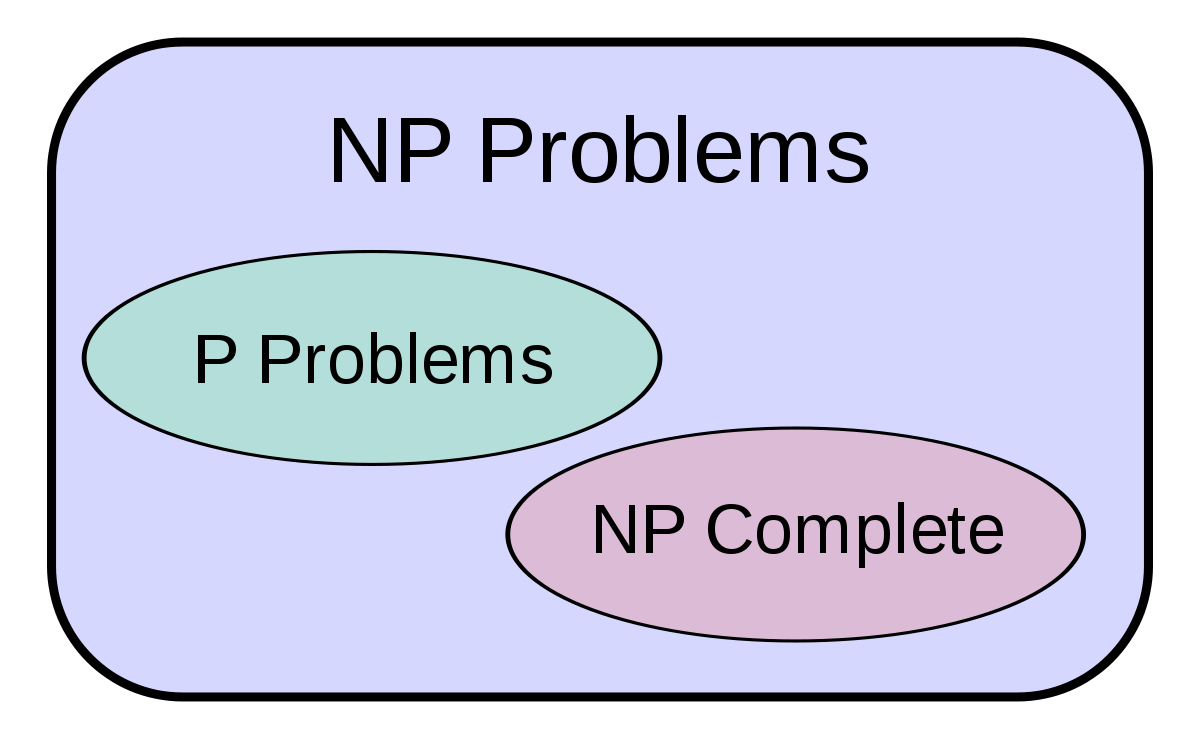
\includegraphics[height=6cm]{img/algorithm-complexity.png}
	\caption{Complessità T(n).}	
\end{figure}

\newpage
	
\section{Ordinamento}

\subsection{Problema dell'Ordinamento (Sorting)}
\texttt{Input}: sequenza di numeri 
\begin{center}
	$a_0 a_1 \dots a_n$;\par
\end{center}
\texttt{Output}: permutazione
\begin{center}
	$a'_0 a'_1 \dots a'_n$
\end{center}
tale che 
\begin{center}
	$a'_0 \leq a'_1 \leq \dots \leq a'_n$
\end{center}

\noindent Vedremo due algoritmi:
\begin{itemize}[noitemsep]
	\item \texttt{InsertionSort};
	\item \texttt{MergeSort}.
\end{itemize}

\subsection{Insertion Sort} \label{insertionsort}
\href{https://en.wikipedia.org/wiki/Insertion_sort}{Insertion Sort} un algoritmo di \emph{sorting incrementale}. Viene applicato naturalmente ad esempio quando si vogliono ordinare le carte nella propria mano in una partita a scala 40: si prende ogni carta a partire da sinistra, e la si posiziona in ordine crescente.\par
\paragraph{Astrazione} Prendiamo ad esempio il seguente array:

\begin{center}
	\begin{tabular}{|l|l|l|l|l|}
		\hline
		5 & 2 & 8 & 4 & 7 \\
		\hline
	\end{tabular}
\end{center}

\noindent Partiamo dal primo elemento: 5. È già ordinato con se stesso, quindi procediamo con il secondo elemento.\par
\noindent Confronto il numero 2 con l'elemento alla sua sinistra: \par
$2 \geq 5$?  No, quindi lo inverto con l'elemento alla sua sinistra, come segue

\begin{center}
	\begin{tabular}{|l|l|l|l|l|}
		\hline
		2 & 5 & 8 & 4 & 7 \\
		\hline
	\end{tabular}
	\hspace{1cm} Key: 
	\begin{tabular}{|l|}
		\hline
		8 \\
		\hline
	\end{tabular}
\end{center}

\noindent La key analizzata è 8. \par
$8 \geq 5$? Sì, quindi è ordinato in modo corretto.

\begin{center}
	\begin{tabular}{|l|l|l|l|l|}
		\hline
		2 & 5 & 8 & 4 & 7 \\
		\hline
	\end{tabular}
	\hspace{1cm} Key: 
	\begin{tabular}{|l|}
		\hline
		4 \\
		\hline
	\end{tabular}
\end{center}

\noindent La key analizzata è 4.\par
$4 \geq 8$? No, quindi lo sposto a sinistra invertendolo con 8.\par 
$4 \geq 5$? No, lo sposto a sinistra invertendolo con 5.\par
$4 \geq 2$? Sì, quindi è nella posizione corretta.

\begin{center}
	\begin{tabular}{|l|l|l|l|l|}
		\hline
		2 & 4 & 5 & 8 & 7 \\
		\hline
	\end{tabular}
	\hspace{1cm} Key: 
	\begin{tabular}{|l|}
		\hline
		7 \\
		\hline
	\end{tabular}
\end{center}

\noindent Key analizzata 7. \par
$7 \geq 8$? No, lo sposto a sinistra invertendolo con 8.\par
$7 \geq 5$? Sì, è nella posizione corretta.\par

\smallskip
\noindent Ottengo l'array ordinato:

\begin{center}
	\begin{tabular}{|l|l|l|l|l|}
		\hline
		2 & 4 & 5 & 7 & 8 \\
		\hline
	\end{tabular}
\end{center}

\newpage

\paragraph{Algorimo} Passiamo ora all'implementazione dell'algoritmo, con uno pseudocodice similare a \texttt{Python}\footnote{\textbf{ATTENZIONE}: verranno usati array con indici
che partono da 1.}\par

\bigskip

\texttt{Input}: $A[1, \twodots ,n]$, $A.length$.

\begin{center}
	È noto che: 
	$A[i] \leq key < A[i+1]$
\end{center}

\paragraph{Pseudocodice} Segue lo pseudocodice dell'\texttt{InsertionSort}.

\begin{codebox}
\Procname{$\proc{Insertion-Sort}(A)$}
\li $n \gets \attrib{A}{length}$
\li \For $j \gets 2$ \To $n$
		\Comment il primo elemento è già ordinato
\li	\Do
		$\id{key} \gets A[j]$ 
			\Comment $A[1 \twodots j-1]$ ordinato
\li		$i \gets j-1$
\li		\While $(i > 0)$ \And $(A[i] > \id{key})$
\li		\Do
			$A[i+1] \gets A[i]$
\li			$i \gets i-1$
		\End
\li		$A[i+1] \gets \id{key}$
	\End
\end{codebox}

\vspace{0.5cm}

Quando il \texttt{while} termina, ci sono due casi: 
\begin{itemize}
	\item[$\circ$] \texttt{i = 0}: tutti gli elementi prima di \texttt{j} 
	sono maggiori di \texttt{key}; \texttt{key} va al primo posto (1);
	\item[$\circ$] \texttt{(i > 0) and (A[i] $\leq$ key)}: \texttt{A[i+1] = key}.
\end{itemize}

\subsubsection{Correttezza di Insertion Sort}

\paragraph{for} \texttt{A[1$\twodots$j-1]} è ordinato e contiene gli 
elementi in \texttt{(1,j-1)} iniziali.

\paragraph{while} \texttt{A[1$\twodots$i]A[i+2$\twodots$j]} ordinato e 
\texttt{A[i+2$\twodots$j] > key}. \par
\vspace{0.5cm}
In uscita abbiamo: 
\begin{itemize}[noitemsep]
	\item[$\circ$] \texttt{j = n+1}; \par
	\item[$\circ$] \texttt{A[1$\twodots$n]} ordinato, come da invariante: 
	vale \texttt{A[1$\twodots$j-1]}	ordinato, e \texttt{j} vale \texttt{n+1}.
\end{itemize}
 
\subsubsection{Complessità di Insertion Sort} \label{is:complessita}
\paragraph{Assunzione} Tutte le istruzioni richiedono un tempo \underline{costante}.

Rivediamo l'algoritmo:

\begin{codebox}
\Procname{\proc{InsertionSort}$(A)$}
\li $n \gets \attrib{A}{length}$
\li \For $j \gets 2$ \To $n$
	\Comment il primo elemento è già ordinato
\li		\Do
			$\id{key} \gets A[j]$ 
			\Comment $A[1 \twodots j-1]$ ordinato
\li			$i \gets j-1$
\li			\While $i > 0$ and $A[i] > \id{key}$
\li				\Do
					$A[i+1] \gets A[i]$
\li					$i \gets i-1$
				\End
\li			$A[i+1] \gets \id{key}$
		\End
\end{codebox}

Diamo il nome $c_0$ alla chiamata del metodo, \texttt{InsertionSort(A)};
A ogni riga numerata, diamo il nome $c_1, c_2,\twodots ,c_8$
\footnote{($c_1$ corrisponde alla riga 1, $c_2$ alla riga 2 e così via).}.\par
Vediamo il \emph{costo} di ogni istruzione:

\begin{itemize}
    \item[] $\boldsymbol{c_0} \rightarrow 1$
    \item[] $\boldsymbol{c_1} \rightarrow 1$
    \item[] $\boldsymbol{c_2} \rightarrow n$
    \item[] $\boldsymbol{c_3} \rightarrow (n-1)$
    \item[] $\boldsymbol{c_4} \rightarrow (n-1)$
    \item[] $\boldsymbol{c_5} \rightarrow \displaystyle\sum_{j=2}^{n} t_j+1$
    \item[] $\boldsymbol{c_6}, \boldsymbol{c_7} \rightarrow \displaystyle\sum_{j=2}^{n} t_j$
    \item[] $\boldsymbol{c_8} \rightarrow (n-1)$
\end{itemize}
 
\begin{displaymath}
    T^{IS}(n) = c_0 + c_1 + c_2n + (c_3+c_4+c_8)(n-1)
    + c_5\displaystyle\sum_{j=2}^{n}(t_j+1) + (c_6+c_7)\displaystyle\sum_{j=2}^{n}t_j
\end{displaymath}

$\boldsymbol{t_j}$ dipende, oltre che da $n$, dall'istanza dell'array
che stiamo considerando.
È chiaro che questo calcolo non da indicazioni precise sull'effettiva
complessità dell'algoritmo.\par

\bigskip
Andiamo ad analizzare i 3 possibili casi:

\begin{enumerate}[label=\emph{\alph*})]
    \item Caso migliore (\ref{is:casomigliore})
    \item Caso peggiore (\ref{is:casopeggiore})
    \item Caso medio (\ref{is:casomedio})
\end{enumerate}

\paragraph{Caso migliore} \label{is:casomigliore}

$\rightarrow A$ ordinato $\Rightarrow t_j = 0 $ $\forall j$

\bigskip
La \textbf{complessità} diventa:
\begin{displaymath}
    T^{IS}_{min}(n) = c_0 + c_1 + c_2n + (c_3+c_4+c_5+c_8)(n-1) 
    = an+b \approx n
\end{displaymath}

Ossia, si comporta come $n$. Il \emph{caso migliore} \textbf{non}
è interessante, visto che è improbabile si presenti.

\paragraph{Caso peggiore} \label{is:casopeggiore}

$\rightarrow A$ ordinato in senso inverso $\Rightarrow \forall j$ $t_j = j-1$ \par
\bigskip
La \textbf{complessità} diventa: 

\begin{displaymath}
    T^{IS}_{max}(n) = c_0 + c_1 + c_2n + (c_3+c_4+c_8)(n-1)
    + c_5\displaystyle\sum_{j=2}^{n}j + (c_6+c_7)
    \displaystyle\sum_{j=2}^{n}(j-1)
\end{displaymath}

Per valutare il costo di $\displaystyle\sum_{j=2}^{n}j$ e di 
$\displaystyle\sum_{j=2}^{n}(j-1)$, usiamo la \textbf{somma di Gauss}: \par

\begin{equation}
    \displaystyle\sum_{i=1}^{n}i = \frac{n(n+1)}{2}
\end{equation}
\newpage
Otteniamo:

\begin{displaymath}
    \displaystyle\sum_{j=2}^{n}j = \frac{n(n+1)}{2}-1
\end{displaymath}

\begin{displaymath}
    \displaystyle\sum_{j=2}^{n}(j-1) = \displaystyle\sum_{i=1}^{n}n = \frac{(n-1)n}{2}
\end{displaymath}

Per finire, ricalcoliamo $T^{IS}_{max}(n)$

\begin{displaymath}
    T^{IS}_{max}(n) = a'n^2+b'n+c' \approx n^2
\end{displaymath}

\paragraph{Caso medio} \label{is:casomedio}
Il caso medio è \emph{difficile da calcolare}, e in una considerevole parte dei casi,
coincide con il caso peggiore.\par
Comunque, l'idea è la seguente:

\begin{align*}
    \frac{\displaystyle\sum_{\text{perm. di input}}T^{IS}(p)}{n!} \approx n^2 && 
        \text{posso pensare che } t_j \cong \frac{j-1}{2}
\end{align*}

\subsection{Divide et Impera}

Un algoritmo di sorting \emph{divide et impera} si può suddividere in 3 fasi:

\begin{description}
    \item[divide] divide il problema dato in sottoproblemi più piccoli;
    \item[impera] risolve i sottoproblemi:
    \begin{itemize}
        \item ricorsivamente;
        \item la soluzione è nota (e.g. array con un elemento);
    \end{itemize}
    \item[combina] compone le soluzioni dei sottoproblemi in una soluzione del 
        problema originale.
\end{description}

\subsection{Merge Sort} \label{mergesort}
\href{https://en.wikipedia.org/wiki/Merge_sort}{Merge Sort}\footnote{Si %
consiglia di dare uno sguardo all'algoritmo anche da altre fonti, poichè presentarlo %
graficamente in \LaTeX, come è stato visto a lezione, non è facile.} è un 
esempio di algoritmo \emph{divide et impera}. Andiamo ad analizzarlo.

\paragraph{Astrazione} Consideriamo il seguente array A.
\begin{center}
	\begin{tabular}{|l|l|l|l||l|l|l|l|}
		\hline
		5 & 2 & 4 & 7 & 1 & 2 & 3 & 6 \\
		\hline
	\end{tabular}
\end{center}

Lo divido a metà, ottenendo due parti separate.

\begin{center}
	\begin{tabular}{|l|l|l|l|}
		\hline
		5 & 2 & 4 & 7 \\
		\hline
	\end{tabular}
	\hspace{1cm}
	\begin{tabular}{|l|l|l|l|}
		\hline
		1 & 2 & 3 & 6 \\
		\hline
	\end{tabular}
\end{center}

Consideriamo il primo, ossia \texttt{A[1$\twodots$4]} (A originale). Divido anche questo a metà.

\begin{center}
	\begin{tabular}{|l|l|}
		\hline
		5 & 2 \\
		\hline
	\end{tabular}
	\hspace{1cm}
	\begin{tabular}{|l|l|}
		\hline
		4 & 7 \\
		\hline
	\end{tabular}
\end{center}

Divido nuovamente a metà, ottenendo:

\begin{center}
	\begin{tabular}{|l|}
		\hline
		5 \\
		\hline
	\end{tabular}
	\hspace{1cm}
	\begin{tabular}{|l|}
		\hline
		2 \\
		\hline
	\end{tabular}
\end{center}

5 e 2 sono due blocchi già ordinati. Scelgo il minore tra i due e lo metto in prima 
posizione, mentre l'altro in seconda posizione, ottenendo un blocco composto da 2 e 5.\par
Riprendo con il blocco composto da 4 e 7. Lo divido in due blocchi da un elemento. Faccio lo stesso procedimento 
fatto per 2 e 5: metto in prima posizione 4 e in seconda posizione 7. La situazione
è la seguente:

\begin{center}
	\begin{tabular}{|l|l|}
		\hline
		2 & 5 \\
		\hline
	\end{tabular}
	\hspace{1cm}
	\begin{tabular}{|l|l|}
		\hline
		4 & 7 \\
		\hline
	\end{tabular}
\end{center}

So che i blocchi ottenuti contengono elementi ordinati. Con questa assunzione, posso ragionare 
nel seguente modo: considero il primo elemento dei due blocchi (2 e 4 in questo caso) e metto 
in prima posizione il minore tra i due. Ora considero il successivo elemento del blocco che è stato scelto e lo stesso elemento dell'altro blocco, e inserisco nell'array l'elemento minore. Continuo fino ad 
ottenere un blocco ordinato.

\begin{center}
	\begin{tabular}{|l|l|l|l|}
		\hline
		2 & 4 & 5 & 7 \\
		\hline
	\end{tabular}
\end{center}

Faccio lo stesso procedimento con la parte di array originale \texttt{A[5$\twodots$8]}, ottenendo

\begin{center}
	\begin{tabular}{|l|l|l|l|}
		\hline
		2 & 4 & 5 & 7 \\
		\hline
	\end{tabular}
	\hspace{1cm}
	\begin{tabular}{|l|l|l|l|}
		\hline
		1 & 2 & 3 & 6 \\
		\hline
	\end{tabular}
\end{center}

A questo punto, i blocchi da 4 contengono elementi tra loro ordinati. Faccio lo stesso ragionamento
usato per comporli, per ottenere l'array originale ordinato. Considero\footnote{Questo procedimento è stato applicato %
anche ai passaggi precedenti; qui è spiegato più rigorosamente.}:
\begin{itemize}[noitemsep]
    \item \texttt{L[1$\twodots$4] $=$ A[1$\twodots$4]}: indice $i = 1$ per scorrerlo;
    \item \texttt{R[1$\twodots$4] $=$ A[5$\twodots$8]}: indice $j = 1$ per scorrerlo;
\end{itemize}

Valuto \texttt{L[i]} e \texttt{R[j]}. \par
\begin{itemize}[noitemsep]
    \item Se \texttt{L[i]} $\leq$ \texttt{R[j]}, inserisco \texttt{L[i]} e incremento \texttt{i}. \par
    \item Altrimenti, inserisco \texttt{R[j]} e incremento \texttt{j}.
    \item Itero finchè entrambi gli indici non sono out of bounds.
\end{itemize}

\paragraph{Pseudocodice} Segue lo pseudocodice del 
\texttt{Merge Sort}.

\begin{codebox}
\Procname{\proc{MergeSort}$(A,p,r)$}
\li \If $p < r$
\li     \Then
            $q \gets \floor{\frac{p + r}{2}}$ 
        \Comment arrotondato per difetto
\li         $\proc{MergeSort}(A,p,q)$
        \Comment ordina \texttt{A[p$\twodots$q]}
\li         $\proc{MergeSort}(A,q+1,r)$
        \Comment ordina \texttt{A[q+1$\twodots$r]}
\li         $\proc{Merge}(A,p,q,r)$
        \Comment ``Merge'' dei due sotto-array 
        \End
\end{codebox}

\begin{codebox}
\Procname{\proc{Merge}$(A,p,q,r)$}
\li $\id{n1} \gets q-p+1$
    \Comment gli indici partono da 1
\li $\id{n2} \gets r-q$
\zi \Comment \kw{L} sotto-array sx, \kw{R} sotto-array dx
\li \For $i \gets 1$ \To $\id{n1}$
\li     \Do
            $L[i] \gets A[p+i-1]$
        \End
\li	\For $j \gets 1$ \To $\id{n2}$
\li		\Do
			$R[j] \gets A[q+j]$
        \End
\li         $L[\id{n1}+1] \gets R[\id{n2}+1] \gets \infty$
\li         $i \gets j \gets 1$
\li         \For $k = p$ \To $r$
\li             \Do
                    \If $L[i] \leq R[j]$
\li                     \Then
                            $A[k] \gets L[i]$
\li                         $i \gets i+1$
\li                     \Else
                    \Comment \texttt{L[i]} $>$ \texttt{R[j]}
\li                            $A[k] \gets R[j]$
\li                         $j \gets j+1$
                        \End
                \End
\end{codebox}

\paragraph{Invarianti e Correttezza}

\textbf{L} e \textbf{R} contengono rispettivamente 
\texttt{A[p$\twodots$q]} e \texttt{A[q+1$\twodots$r]}. 
L'indice \texttt{k} scorre \texttt{A}. Il sotto-array \texttt{A[p$\twodots$k-1]}
è ordinato, e contiene \texttt{L[1$\twodots$i-1]} e \texttt{R[1$\twodots$j-1]}.

\begin{center}
    $A[p \twodots k-1] \leq L[i \twodots n1], R[j \twodots n2]$ \\
    $\Downarrow$ \\
    $A[p \twodots k-1] = A[p \twodots r+1-1] \implies A[p \twodots r] \text{ ordinato}$
\end{center}

\paragraph{Dimostrazione per induzione su r-p} 
\begin{itemize}
    \item[$\Rightarrow$] Se $r-p == 0 $ (oppure $-1$) abbiamo al
    più un elemento $\implies$ array già ordinato.
    \item[$\Rightarrow$] Se $r-p > 0$, vale 
    $$\#\text{elem}(A[p \twodots q]),\#\text{elem}(A[q+1 \twodots r]) 
    < \#\text{elem}(A[p \twodots r])$$
    Per ipotesi induttiva:
    \begin{itemize}
        \item \texttt{Merge-sort(A,p,q)} ordina \texttt{A[p$\twodots$q]};
        \item \texttt{Merge-sort(A,q+1,r)} ordina \texttt{A[q+1$\twodots$r]}; \par
        Per correttezza di \texttt{Merge()}, dopo la sua chiamata ottengo 
        \texttt{A[p$\twodots$r]} ordinato.
    \end{itemize}
\end{itemize}  
\subsubsection{Approfondimento sull'Induzione}
\paragraph{Induzione ordinaria} 
Proprietà $P(n)$, e.g.  $P(n) = $ ``Se $n$ è pari, $n+1$ è dispari'' oppure 
``tutti i grafi con $n$ nodi \dots ''.\par
Per dimostrare che $P(n)$ vale per ogni $n$
\begin{itemize}
	\item $P(0)$: \textbf{caso base};
	\item assumo vera $P(n) \rightarrow $ dimostro $P(n+1)$, allora $P(n)$
	è vera per ogni $n$.
\end{itemize}

\paragraph{Induzione completa}
\begin{itemize}
	\item $\big[ P(0) \big]$ (non necessaria, è un'istanza del passo successivo);
	\item dimostro $P(m) \ \forall m<n \rightarrow $ vale $P(n) \ \forall n$.  
\end{itemize}

\subsubsection{Complessità di Merge Sort}

$n =$ \verb|#| elementi da ordinare\footnote{Il simbolo \# verrà usato per indicare la cardinalità di un insieme.}

\paragraph{Merge(A, p, q, r)}
\begin{itemize}
	\item[] \textbf{inizializzazione}: $a'n+b'$;
	\item[] \textbf{ciclo}: $a'n+b'$;
\end{itemize}

Sommandoli, ottengo una complessità all'incirca di:
\begin{displaymath}
	T^{merge}(n) = an+b
\end{displaymath}

Nel dettaglio: 

\[ T^{MS}(n) =
\begin{cases}
	c_0       & \quad \text{se } n \leq 1 \\
	T^{MS}(n_1)+T^{MS}(n_2)+T^{merge}(n)  & \quad \text{altrimenti}
\end{cases}
\]

\begin{center}
	$\Downarrow$ \\
\end{center}

\[ T^{MS}(n) =
\begin{cases}
c_0       & \quad \text{se } n \leq 1 \\
T^{MS}(n_1)+T^{MS}(n_2)+an+b  & \quad \text{altrimenti}
\end{cases}
\]

con 

\begin{itemize}
	\item[] $n_1 = \floor{\frac{n}{2}}$
	\item[] $n_2 = \ceil{\frac{n}{2}}$
\end{itemize}

\[ T^{MS}(n) =
\begin{cases}
c_0       & \quad \text{se } n \leq 1 \\
T^{MS}(\floor{\frac{n}{2}})+T^{MS}(\ceil{\frac{n}{2}})+an+b  & \quad \text{altrimenti}
\end{cases}
\]

\begin{center}
	\begin{tikzpicture}[rec,level/.style={level distance=25mm, sibling distance=55mm/#1}]
		\node (a) {$T^{MS}(n)$\\$an+b$}
		child {node (b) {$T^{MS}(n_1)$\\$an_1+b$}
			child {node (d) {$T^{MS}(n_{11})$\\$an_{11}+b$}
				child {node (d1) {$\vdots$}[no edge from this parent]
					child {node (d11) {$c_0$}}
				}
				child {node (d2) {$\vdots$}[no edge from this parent]
					child {node (d12) {$c_0$}}
				}
			}
			child {node (e) {$T^{MS}(n_{12})$\\$an_{12}+b$}
				child {node (e1) {$\vdots$}[no edge from this parent]
					child {node (e11) {$c_0$}}
				}
				child {node (e2) {$\vdots$}[no edge from this parent]
					child {node (e12) {$c_0$}}
				}
			}
		}
		child {node (c) {$T^{MS}(n_2)$\\$an_2+b$}
			child {node (f) {$T^{MS}(n_{21})$\\$an_{21}+b$}
				child {node (f1) {$\vdots$}[no edge from this parent]
					child {node (f11) {$c_0$}}
				}
				child {node (f2) {$\vdots$}[no edge from this parent]
					child {node (f12) {$c_0$}}
				}
			}
			child {node (g) {$T^{MS}(n_{22})$\\$an_{22}+b$}
				child {node (g1) {$\vdots$}[no edge from this parent]
					child {node (g11) {$c_0$}}
				}
				child {node (g2) {$\vdots$}[no edge from this parent]
					child {node (g12) {$c_0$}
					}
				}
			}
		};
	\end{tikzpicture}
\end{center}

Otteniamo $c_0$ ripetuto $n$ volte all'ultimo livello dell'albero. L'altezza dell'albero è circa 
$\log_2 n$. Vediamo nel dettaglio la complessità nelle varie iterazioni.
\begin{itemize}
	\item[] $\boldsymbol{i=0}$ \hspace{0.5cm} $an+b$
	\item[] $\boldsymbol{i=1}$ \hspace{0.5cm} $a(n_1+n_2)+2b \approx an+2b$
	\item[] $\boldsymbol{i=2}$ \hspace{0.5cm} $a(n_{11}+n_{12}+n_{21}+n_{22})+4b \approx an+4b$
	\item[] \dots
	\item[] $\boldsymbol{i=h}$ \hspace{0.5cm} $c_0n$
\end{itemize}

Poniamo $n=2^h$. Abbiamo

\begin{align*}
	T^{MS}(n) 	& = \displaystyle\sum_{i=0}^{h-1}(an+2^ib)+c_0n \\
				& = anh+b\displaystyle\sum_{i=0}^{h-1}2^i && \text{($h= \log_2n$)}\\
				& = an \log_2n + b2^h - b + c_0n && \text{($2^h=n$)} \\
				& = an \log_2n + (b+c_0)n - b
\end{align*}
\begin{displaymath}
	T^{MS}(n) = an \log_2n + b''n + c'' \approx n \log_2n
\end{displaymath}

\subsection{Confronto tra Insertion Sort e Merge Sort}

\begin{gather*}
	T^{IS}(n) = a'n^2 + b'n + c' \\
	T^{MS}(n) = a''n \log_2n + b''n + c''
\end{gather*}

Posso calcolare il limite del rapporto:
\begin{displaymath}
	\lim_{n \to +\infty} \frac{T^{MS}(n)}{T^{IS}(n)} = \lim_{n \to +\infty} \frac{a''n \log_2n + b''n + c''}{a'n^2 + b'n + c'} = 0
\end{displaymath}

Per definizione
\begin{gather*}
	\forall \varepsilon > 0 \ \exists n_0 : \forall n \geq n_0 \quad \frac{T^{MS}(n)}{T^{IS}(n)} < \varepsilon \\
	\Downarrow \\
	T^{MS}(n) < \varepsilon T^{IS}(n) = \frac{T^{IS}}{m} \qquad \text{(Ponendo, ad esempio, $\varepsilon = \frac{1}{m}$)}
\end{gather*}

Detto a parole, c'è un certo $n$ oltre il quale, ad esempio, \texttt{MergeSort} su un \emph{Commodore 64} 
esegue più velocemente di un \texttt{InsertionSort} su una macchina moderna. Possiamo vedere una comparazione tra i due algoritmi nella seguente tabella.
\begin{center}
	\begin{tabular}{l|c|c}
		$n$ & $T^{IS}(n)=n^2$ & $T^{MS}(n)=n \log n$ \\
		\hline
		10 & $0.1ns$ & $0.033ns$ \\
		\hline
		1000 & $1ms$ & $10\mu s$ \\
		\hline
		$10^6$ & 17 minuti & $20ms$ \\
		\hline
		$10^9$ & 70 anni & $30s$ \\
	\end{tabular}
\end{center} 
\section{Limiti Asintotici e Ricorrenze}

\subsection{Notazione Asintotica}
Il \textbf{tempo di esecuzione} è difficile da calcolare, come visto nella sezione \ref{is:complessita}. 
Il modo in cui è stato calcolato è pieno di dettagli ``inutili''.\par
Rivediamo le complessità di \texttt{Insertion Sort} e \texttt{Merge Sort}:
\begin{gather*}
	T^{IS} = an^2 + bn + c \\
	T^{MS} = an \log_2 n + bn + c
\end{gather*}

A noi interessa calcolare $T(n)$ per $n$ ``grande''. Non consideriamo le costanti moltiplicative, che sono non fondamentali. Ecco una lista di possibili complessità ordinate in senso decrescente (le prime due categorie appartengono alla classe degli \emph{NP problems}, ossia non trattabili):

\begin{itemize}[noitemsep]
	\item $3^n$
	\item $2^n$
	\medskip
	\item $n^k$
	\item $n^2$
	\item $n \log n$
	\item $n$
	\item $\log n$
	\item $1$
\end{itemize}

Prendiamo in esame due funzioni: $f(n)$, $g(n)$:

\begin{displaymath}
f, g: \mathbb{R}^+ \rightarrow \mathbb{R}^+
\end{displaymath}

\begin{itemize}
	\item $f(n)$ è la funzione in esame della complessità del nostro problema P;
	\item $g(n)$ è la funzione che, moltiplicata per un'opportuna costante $c_i$, dopo un certo $n$, fa da 
	limite superiore o inferiore per ogni punto di $f(n)$.
\end{itemize}
\newpage
\subsubsection{Limite Asintotico Superiore}
Data $g(n)$, indichiamo con $O \big(g(n) \big)$ il \emph{limite asintotico superiore}, definito come segue:
\begin{displaymath}
	O \big(g(n) \big) = \{ f(n) : \exists c > 0 \quad \exists n_0 \in \mathbb{N} : \forall n \geq n_0 \quad (0 \leq) f(n) \leq c \cdot g(n) \}
\end{displaymath}

\begin{figure}[!htb]
	\centering
	\includegraphics[width=0.80\textwidth]{img/plots/plotO.png}
	\caption{Rappresentazione del limite asintotico superiore per $f(n)$}
\end{figure}

\paragraph{Esempi}
\begin{itemize}
	\item $f_1(n) = 2n^2 + 5n + 3 = O \big(g(n^2) \big)$ ? Sì. \par
	Deve valere $f_1(n) < cn^2 \qquad \exists c > 0, \ n \geq n_0$ \par
	Ipotizziamo $c = 3$
	\begin{align*}
		2n^2 + 5n + 3 & \leq 3n^2 \\
		n^2 - 5n - 3 & \geq 0 \\
		\frac{5 \pm \sqrt{2 \cdot 5 + 12}}{2} = \frac{5 \pm \sqrt{37}}{2} \cong 5.54 && \text{(Non considero la soluzione} \\ && \text{negativa, poiché siamo in } \mathbb{R}^+ \text{)}
	\end{align*}
	\begin{center}
		\includegraphics[height=6cm]{img/parabola-plot1.png}
	\end{center}
	
	Prendo $c = 3$ e $n_0 = 6$. Vale dunque:
	\begin{displaymath}
		f_1(n) \leq cn^2 \quad \forall n \geq n_0
	\end{displaymath}

	\item $f_1(n) = O \big(g(n^3) \big)$ ? Sì. \par
	$c = 3 $\par
	$n_0 = 6 \quad \forall n \geq n_0$ \par
	$f_1(n) \leq cn^2 \leq cn^3$
	
	\item $f_2(n) = 2 + \sin (n) = O(1)$ ? Sì. \par
	$-1 \leq \sin (n) \leq 1$ \par
	$1 \leq f_2(n) \leq 3$ \par
	Vale la seguente
	\begin{gather*}
		\exists c > 0 \quad \exists n_0 : \forall n \geq n_0 \quad f_2(n) \leq c \cdot 1 \\
		\text{ok per } c = 3, \ n_0 = 0
	\end{gather*}
\end{itemize}

\newpage
\subsubsection{Limite Asintotico Inferiore}
Data $g(n)$, indichiamo con $\Omega \big(g(n) \big)$ il \emph{limite asintotico inferiore}, definito come segue:
\begin{displaymath}
	\Omega \big(g(n) \big) = \{ f(n) : \exists c > 0 \quad \exists n_0 \in \mathbb{N} : \forall n \geq n_0 \quad c \cdot g(n) \leq f(n) \}
\end{displaymath}

\begin{figure}[!htb]
	\centering
	\includegraphics[width=0.80\textwidth]{img/plots/plotomega.png}
	\caption{Rappresentazione del limite asintotico inferiore per $f(n)$}
\end{figure}

\paragraph{Esempi}
\begin{itemize}
	\item $f_1(n) = 2n^2 + 5n + 3 = \Omega \big(g(n^2) \big)$ ? Sì.\par
	Deve valere: \par
	\begin{displaymath}
		\exists c > 0 \quad \exists n_0 : \forall n \geq n_0 \quad cn^2 \leq 2n + 5n + 3
	\end{displaymath}
	Basta porre $c = 1$, $n_0 = 0$.
	
	\item $f_2(n) = 2 + \sin (n) = \Omega (1)$ ? Sì.
	\begin{displaymath}
		1 \leq f_2(n) \leq 3 \quad c = 1, \ n_0 = 0
	\end{displaymath}
\end{itemize}

\subsubsection{Limite Asintotico Stretto}
Data $g(n)$, indichiamo con $\Theta \big( g(n) \big)$ il \emph{limite asintotico stretto}, definito come segue:
\begin{multline*}
	\Theta \big( g(n) \big) = \{ f(n) : \exists c_1, c_2 > 0 \quad \exists n_0 \in \mathbb{N} : \forall n \geq n_0 \\ 
	c_1 \cdot g(n) \leq f(n) \leq c_2 \cdot g(n) \}
\end{multline*}

\begin{figure}[!htb]
	\centering
	\includegraphics[width=0.80\textwidth]{img/plots/plottheta.png}
	\caption{Rappresentazione del limite asintotico stretto per $f(n)$}
\end{figure}

\paragraph{Esempi}
\begin{align*}
	f_1(n) = & 2n^2 + 5n + 3 = \Theta (n^2) && f_1(n) \neq \Theta (n^3) \\
	& c_1 = 1 \quad c_2 = 3 \quad n_0 = 6 && f_1(n) = O(n^3) \\
	f_2(n) = & 2 + \sin (n) = \Theta (1) && f_1(n) \neq \Omega (n^3) \\
	& c_1 = 1 \quad c_2 = 3 \quad n_0 = 0 && \qquad \Downarrow \\
	& && \frac{f_1(n)}{n_3} \rightarrow 0
\end{align*}
\newpage
\subsection{Metodo del Limite}
Siano $f(n),\ g(n) > 0 \quad \forall n$ \par \medskip
Se $\exists \lim_{n \to +\infty} \frac{f(n)}{g(n)}$, allora:

\begin{enumerate}
	\item Se $\lim_{n \to +\infty} \frac{f(n)}{g(n)} = k > 0$ allora $f(n) = \Theta \big( g(n) \big)$.
	
	\item Se $\lim_{n \to +\infty} \frac{f(n)}{g(n)} = 0$ allora $f(n) = O \big( g(n) \big)$ e 
	$f(n) \neq \Omega \big( g(n) \big)$.
	
	\item Se $\lim_{n \to +\infty} \frac{f(n)}{g(n)} = \infty$ allora $f(n) = \Omega \big( g(n) \big)$ e 
	$f(n) \neq O \big( g(n) \big)$.
\end{enumerate}

\paragraph{Dimostrazione}
\begin{enumerate}
	\item Sia $\lim_{n \to +\infty} \frac{f(n)}{g(n)} = k > 0$
	\begin{align*}
	& \Rightarrow \forall \varepsilon > 0 \quad \exists n_0 : \forall n \geq n_0 \quad \abs{\frac{f(n)}{g(n)} - k} \leq \varepsilon \\
	& \Rightarrow - \varepsilon \leq \frac{f(n)}{g(n)} - k \leq \varepsilon \\
	& \Rightarrow k - \varepsilon \leq \frac{f(n)}{g(n)} \leq k + \varepsilon \\
	& \Rightarrow (k - \varepsilon)g(n) \leq f(n) \leq (k + \varepsilon)g(n) \qquad \text{per } 0 < \varepsilon < k \\
	& \Rightarrow f(n) = \Theta \big( g(n)\big)
	\end{align*}
	
	\item Sia $\lim_{n \to +\infty} \frac{f(n)}{g(n)} = 0$ 
	\begin{align*}
	& \Rightarrow \forall \varepsilon > 0 \quad \exists n_0 : \forall n \geq n_0 \quad \frac{f(n)}{g(n)} \leq \varepsilon \\
	& \Rightarrow f(n) \leq  \varepsilon g(n) \\
	& \Rightarrow f(n) = O \big( g(n) \big)
	\end{align*}
	Sia $f(n) = \Omega \big( g(n) \big)$
	\begin{align*}
	& \Rightarrow \exists c > 0 \quad \exists n_0 \in \mathbb{N} : \forall n \geq n_0 \quad c g(n) \leq f(n) \\
	& \Rightarrow \text{Impossibile, infatti sia } \varepsilon = \frac{c}{2} > 0 \\
	& \Rightarrow \exists n_1 \in \mathbb{N} : \forall n \geq n_1 \quad f(n) \leq \frac{c}{2} g(n) < c g(n) \\
	& \Rightarrow \text{Contraddizione!}
	\end{align*}
	
	\item Si dimostra in modo analogo al punto (2)
\end{enumerate}

\subsection{Proprietà Generali}
\begin{itemize}
	\item $f(n) = a_kn^k + a_{k-1}n^{k-1} + \dots + a_1n + a_0 = \Theta (n^k)$
	\item $h \neq k \quad \Theta (n^h) \neq \Theta (n^k)$
	\item $a \neq b \quad \Theta (a^k) \neq \Theta (b^n)$
	\item $h \neq k \quad \Theta (a^{n+h}) = \Theta (a^{n+k})$
	\item $a \neq b \quad \Theta (\log_an) = \Theta (\log_bn)$
\end{itemize} 
In generale
\begin{gather*}
	O(1) \subseteq O(\log n) \subseteq O(n) \subseteq O(n \log n) \subseteq O(n^2) \subseteq \dots
\end{gather*}
\subsection{Complessità di un Problema}
Dato un problema P \{INPUT $\rightarrow$ OUTPUT\}, la \textbf{complessità} di P è la 
complessità dell'algoritmo più efficiente che risolve P.

\paragraph{Limite superiore per complessità di P} Se A è un algoritmo per P con
complessità  $O \big( f(n) \big)$, allora P è $O \big( f(n) \big)$.

\paragraph{Limite inferiore per complessità di P}
Se ogni algoritmo che risolve P ha complessità $\Omega \big( f(n) \big)$, allora 
P ha complessità $\Omega \big( f(n) \big)$
\bigskip

$\implies$ se P è $O \big( f(n) \big)$ e $\Omega \big( f(n) \big) \Rightarrow$ P è $\Theta \big( f(n) \big)$ 

\subsubsection{Esempio: limite inferiore per ordinamento basato su scambi di elementi contigui}

\paragraph{Def (inversione)} Dato \texttt{A[1$\twodots$n]}, una \emph{inversione} è una coppia $(i,j)$
con $i,j \in [1,n]$ con $i < j$ e \texttt{A[i]} $>$ \texttt{A[j]}.\par \medskip
Operazione disponibile: \texttt{A[k]} $\leftrightarrow$ \texttt{A[k+1]} (scambio tra gli elementi in posizione
$k$ e $k+1$).
\begin{align*}
	\# inv(A) & = \text{numero di inversioni di } A \\
	& = \Big{\vert} \ \{ (i,j) : 1 \leq i \leq j \leq n, \ A[i] > A[j] \} \ \Big{\vert}
\end{align*}

\begin{enumerate}
	\item A è ordinato sse $\# inv(A) = 0$;
	\item A è ordinato in senso inverso sse 
	\begin{displaymath}
		\displaystyle\sum_{j=2}^{n}j-1 = \displaystyle\sum_{j=1}^{n-1}j = \frac{n(n-1)}{2}
	\end{displaymath}
	Ossia, $\# inv(A)$ è massimizzato.
\end{enumerate}

Vediamo cosa succede alle coppie $(i,j)$ e a $\# inv(A)$ nel caso avvenga uno scambio \texttt{A[k]}
$\leftrightarrow$ \texttt{A[k+1]}.

\begin{itemize}
	\item $i,j \neq k$ e $i,j \neq k+1 \implies (i,j)$ è inversione prima sse è inversione dopo;
	\item $i = k, \ j = k+1$
	\[ \implies
	\begin{cases}
		A[i] < A[j] & \quad +1 \text{ inversione} \\
		A[i] = A[j] & \quad \# inv(A) \text{ non cambia} \\
		A[i] > A[j] & \quad -1 \text{ inversione}
	\end{cases}
	\]
	\item $i = k$ oppure $i = k+1$, $j > k+1 \implies (k,j)$ è inversione prima sse $(k+1,j)$ è
	inversione dopo;
	\item $j = k$ oppure $j = k+1$, $i < k$, analogo al caso precedente.
\end{itemize}

Per concludere, possiamo dire che l'operazione \texttt{A[k]} $\leftrightarrow$ \texttt{A[k+1]}
riduce $\# inv(A)$ al massimo di 1.
\begin{displaymath}
	\implies \text{qualunque algoritmo di ordinamento basato su scambi è } \Omega \Big(\frac{n(n-1)}{2} \Big) = \Omega (n^2)
\end{displaymath}

\subsection{Soluzione di Ricorrenze}
Abbiamo visto per \texttt{MergeSort} la complessità nel modo seguente:

\begin{codebox}
	\Procname{$\proc{MergeSort}(A,p,r)$}
	\li \If $p < r$
	\li     \Then
	$q \gets \floor{\frac{(p + r)}{2}}$ 
	\li         $\proc{MergeSort}(A,p,q)$
	\li         $\proc{MergeSort}(A,q+1,r)$
	\li         $\proc{Merge}(A,p,q,r)$
	\Comment complessità $an + b$
	\End
\end{codebox}

\[ T^{MS}(n) =
\begin{cases}
c_0       & \quad \text{se } n \leq 1 \\
T^{MS}(\floor{\frac{n}{2}})+T^{MS}(\ceil{\frac{n}{2}}) + an + b  & \quad \text{se } n>1
\end{cases}
\]

È stato tuttavia un approccio non molto preciso. Ci sono due metodi per risolvere precisamente 
i problemi di ricorrenza:
\begin{itemize}[noitemsep]
	\item \emph{Metodo di sostituzione} (\ref{ricorrenze:sostituzione});
	\item \emph{Master Theorem} (\ref{mastertheorem}).
\end{itemize}

\subsubsection{Metodo di Sostituzione} \label{ricorrenze:sostituzione}
Dato una ricorrenza, si può provare a ``indovinare'' la soluzione e dimostrare che è corretta, oppure si può sviluppare l'\emph{albero %
delle ricorrenze}:
\begin{itemize}
	\item \emph{radice}: chiamata di cui vogliamo la complessità;
	\item per ogni nodo:
	\begin{itemize}
		\item[$\rightarrow$] costo della parte non ricorsiva;
		\item[$\rightarrow$] un figlio per ogni chiamata.
	\end{itemize}
\end{itemize}

\paragraph{Esempio} 

\[ T(n) =
\begin{cases}
4       & \quad \text{se } n = 1 \\
2T(\dfrac{n}{2})+ 6n  & \quad \text{se } n>1
\end{cases}
\]

In generale, si può benissimo trascurare il caso base per poter ottenere espressioni meno verbose, in questo 
caso otterremmo:
\begin{displaymath}
	T(n) = 2T(\frac{n}{2})+ 6n
\end{displaymath}

Costruendo l'albero delle ricorrenze si intuisce già la soluzione:
\begin{center}
	\begin{tikzpicture}[rec]
	\node (a) {$T(n)$\\$6n$}
	child {node (b) {$T(\dfrac{n}{2})$\\$6 \dfrac{n}{2}$}
		child {node (d) {$T(\dfrac{n}{4})$\\$6 \dfrac{n}{4}$}
			child {node (d1) {$\vdots$}[no edge from this parent]
				child {node (d11) {$4$}}
			}
			child {node (d2) {$\vdots$}[no edge from this parent]
				child {node (d12) {$4$}}
			}
		}
		child {node (e) {$T(\dfrac{n}{4})$\\$6 \dfrac{n}{4}$}
			child {node (e1) {$\vdots$}[no edge from this parent]
				child {node (e11) {$4$}}
			}
			child {node (e2) {$\vdots$}[no edge from this parent]
				child {node (e12) {$4$}}
			}
		}
	}
	child {node (c) {$T(\dfrac{n}{2})$\\$6 \dfrac{n}{2}$}
		child {node (f) {$T(\dfrac{n}{4})$\\$6 \dfrac{n}{4}$}
			child {node (f1) {$\vdots$}[no edge from this parent]
				child {node (f11) {$4$}}
			}
			child {node (f2) {$\vdots$}[no edge from this parent]
				child {node (f12) {$4$}}
			}
		}
		child {node (g) {$T(\dfrac{n}{4})$\\$6 \dfrac{n}{4}$}
			child {node (g1) {$\vdots$}[no edge from this parent]
				child {node (g11) {$4$}}
			}
			child {node (g2) {$\vdots$}[no edge from this parent]
				child {node (g12) {$4$}
				}
			}
		}
	};
	
	\node[left=5 of a]  (ln1) {$6n$}[no edge from this parent]
	child {node (ln2) {$6n$}[no edge from this parent]
		child {node (ln3) {$6n$}[no edge from this parent]
			child {node (ln4) {}[no edge from this parent]
				child {node (ln5) {$4n$}}}}};
	
	\coordinate (h) at ($(g12)+(1,0)$);
	
	\draw[<->] 
	(h) -- (h|-a.east) node [midway, fill=white] {$\log_2 n$};
	
	\draw[dashed]    
	($(a.west)+(-1em,0)$) -- (ln1);
	\draw[dashed]    
	($(b.west)+(-1em,0)$) -- (ln2.east);
	\draw[dashed]    
	($(d.west)+(-1em,0)$) -- (ln3);
	\draw[dashed]    
	($(d11.west)+(-1em,0)$) -- (ln5);
	\end{tikzpicture}
\end{center}

Per essere sicuri della soluzione, facciamo il procedimento per intero.
Proviamo a ``indovinare'' la soluzione. Assomiglia a \texttt{MergeSort},
quindi ipotizziamo abbia una complessità con un andamento simile 
\begin{displaymath}
	T(n) = an \log n + bn + c
\end{displaymath}
Facciamo la prova induttiva.

\begin{align*}
	(n = 1) \quad T(1) & = 4 \\
	& = a \cdot 1 \cdot \log 1 + b \cdot 1 + c  && (\log 1 = 0)\\
	& = b + c && \text{ok se } b + c = 4 \\
	(n > 1) \quad T(n) & = 2T \big( \frac{n}{2} \big) + 6n \\
\end{align*}
\begin{align*}
	\text{Per ipotesi induttiva} \\
	T \big( \frac{n}{2} \big) & = a \frac{n}{2} \cdot \log \frac{n}{2} + b \frac{n}{2} + c \\
	\text{Calcolo ora } T(n) \\
	T(n) & = an \log_2 \frac{n}{2} + bn + 2c + 6n = \\
	& = an \log_2n - an \log_22 + bn + 6n + 2c =  && (\log_22 = 1)\\
	& = an \log_2n + n(b + 6 - a) + 2c = \\
	& = an \log_2n + bn + c \\
	& \qquad \Downarrow
\end{align*}
\begin{align*}
	b + 6 - a = b \Rightarrow \ & a = 6 \\
	2c = c \Rightarrow \ & c = 0 \\
	& b + c = 4 \Rightarrow b = 4 \\
	T(n) &= an \log n + bn + c \\
	&= 6n \log n + 4n
\end{align*}
\paragraph{Esercizio (importante)} 
\begin{align*}
	T(n) & = 2T\Big(\frac{n}{2}\Big) + 6n \\
		& = 2T\Big(\frac{n}{2}\Big) + \Theta (n) = \Theta (n \log n) \\
		\text{vale } \exists c & > 0 \ \exists n_0 : \forall n \geq n_0 \Rightarrow \Theta(n) \leq cn
\end{align*}
Voglio dimostrare che 
\begin{enumerate}
	\item $T(n) = O(n \log n)$
	\item $T(n) = \Omega (n \log n)$
\end{enumerate}

\subparagraph{1.} $T(n) = O(n \log n)$
\begin{displaymath}
	\text{significa che } \exists d > 0 \ \exists n_1 \in \mathbb{N} \ \vert \ T(n) \leq dn \log n \quad \forall n \geq n_1
\end{displaymath}
Dimostro per induzione $T(n) \leq dn \log n \quad \forall n \geq n_1$.\par
Ometto il caso base, poiché non è molto interessante (mi basterebbe aumentare ulteriormente $d$ per avere
un valore accettabile).
\begin{align*}
	T(n) & \leq 2T\Big(\frac{n}{2}\Big) + cn && \text{ip. induttiva } T\Big(\frac{n}{2}\Big) = d \frac{n}{2} \log \frac{n}{2} \\
	& \leq 2 \cdot \frac{n}{2} d \log \frac{n}{2} + cn && \Big(\log \frac{n}{2} = \log n - \log 2\Big) \\
	& = dn \log n - dn \log 2 + cn \\
	& = dn \log n - n(d \log 2 - c) \leq dn \log n \\
	& \Rightarrow - n(d \log 2 - c) \leq 0 \\
	& n(d \log 2 - c) \geq 0 \\
	& d \log 2 - c \geq 0 \\
	& \qquad d \geq \frac{c}{\log 2}
\end{align*}

\subparagraph{2.} $T(n) = \Omega (n \log n)$ è analoga.
\[
	\exists \delta > 0 : \forall n > n_0 \Rightarrow T(n) \geq \delta n \log n
\]
Ho l'ipotesi induttiva $T(\frac{n}{2}) \geq \delta \frac{n}{2} \log \frac{n}{2}$
\begin{align*}
	T(n) & \geq 2\delta \frac{n}{2} \log \frac{n}{2} + cn = \\
	& = \delta n \log n - \delta n \log 2 + cn = \\
	& = \delta n \log n + n(c - \delta \log 2) \geq \delta n \log n \\
	& \quad \text{Deve valere } c - \delta \log 2 \geq 0 \\
	& \quad \Rightarrow 0 < \delta \leq \frac{c}{\log 2}
\end{align*}
\paragraph{Esercizio} $T(n) = T\big(\frac{n}{3} \big) + T\big(\frac{2n}{3} \big) + \Theta (n)$
$\quad (\Theta (n) \leq c \cdot n)$\par
Ipotizzo un andamento simile a Merge Sort: $\Theta (n \log n)$. Dimostro:  
\begin{enumerate}
	\item $T(n) = O(n \log n)$
	\item $T(n) = \Omega (n \log n)$
\end{enumerate}

\subparagraph{1.} $T(n) = O(n \log n)$
$$\exists d > 0 : \forall n > n_0 \Rightarrow T(n) \leq dn \log n$$
Ometto il caso base. L'ipotesi induttiva è la seguente:
\[ 
	T(n) \leq d \frac{n}{3} \log \frac{n}{3} + d \frac{2n}{3} \log \frac{2n}{3} + cn
\]
Procedo con i calcoli \dots
\begin{align*}
	T(n) & \leq T\Big(\frac{n}{3} \Big) + T\Big(\frac{2n}{3} \Big) + cn \\
	& \leq d \frac{n}{3} \log \frac{n}{3} + d \frac{2n}{3} \log \frac{2n}{3} + cn = \\
	& = d \frac{n}{3} \Big(\log n - \log 3 \Big) + d \frac{2n}{3} \Big(\log n - \log \frac{2}{3} \Big) + cn = \\
	& = dn \log n - \frac{dn}{3} \Big( \log 3 - 2 \log \frac{2}{3} \Big) + cn = \\
	& = dn \log n - \frac{dn}{3} \Big( \log 3 - \log \frac{4}{9} \Big) + cn = \\
	& = dn \log n - n \Big( \frac{d}{3} \log \frac{27}{4} - c \Big) \leq dn \log n\\
	& \quad \frac{d}{3} \log \frac{27}{4} - c \geq 0 \\
	& \Rightarrow d \geq \frac{3c}{\log \frac{27}{4}} \qquad (\log \frac{27}{4} > 1 \text{ poiché } arg > 1)
\end{align*}

\subparagraph{2.} $T(n) = \Omega (n \log n)$ è analoga %$\Rightarrow \text{vale } T(n) = \Theta (n \log n)$
$$\exists \delta > 0 : \forall n > n_0 \Rightarrow T(n) \geq \delta n \log n $$
L'ipotesi induttiva è la seguente:
\[ 
	T(n) \geq \delta \frac{n}{3} \log \frac{n}{3} + \delta \frac{2n}{3} \log \frac{2n}{3} + cn
\]
Calcoli \dots
\begin{align*}
	T(n) & \geq T\Big(\frac{n}{3} \Big) + T\Big(\frac{2n}{3} \Big) + cn \\
	& \geq \delta \frac{n}{3} \log \frac{n}{3} + \delta \frac{2n}{3} \log \frac{2n}{3} + cn = \\
	& = \delta \frac{n}{3} \Big(\log n - \log 3 \Big) + \delta \frac{2n}{3} \Big(\log n - \log \frac{2}{3} \Big) + cn = \\
	& = \delta n \log n + \frac{\delta n}{3} \Big( - \log 3 + 2 \log \frac{2}{3} \Big) + cn = \\
	& = \delta n \log n + \frac{\delta n}{3} \Big( - \log 3 + \log \frac{4}{9} \Big) + cn = \\
	& = \delta n \log n + n \Big( - \frac{\delta}{3} \log \frac{27}{4} + c \Big) \geq \delta n \log n\\
	& \quad - \frac{\delta}{3} \log \frac{27}{4} + c \geq 0 \\
	& \quad \Rightarrow 0 < \delta \leq \frac{3c}{\log \frac{27}{4}}
\end{align*}
\subsubsection{Master Theorem} \label{mastertheorem}
Dato un problema con \texttt{size} $n$, vogliamo dividerlo in $a$ sottoproblemi 
con \mbox {\texttt{size} $\frac{n}{b}$}. Otteniamo la seguente ricorrenza (ricordiamo che
il caso base è omesso per semplicità):
\[
    T(n) = a \cdot T\Big(\frac{n}{b}\Big) + f(n)
\]
con $a \geq 1, \ b > 1$, allora possiamo confrontare
\begin{itemize}
    \item $f(n)$;
    \item $n^{\log_b a}$.
\end{itemize}
Tre possibili casi:
\begin{enumerate}
    \item Se $f(n) = O(n^{\log_b a - \varepsilon})$ per qualche $\varepsilon > 0$,
    allora $$T(n) = \Theta \big( n^{\log_b a} \big)$$
    
    \item Se $f(n) = \Theta (n^{\log_b a})$ allora 
    $$T(n) = \Theta \big( n^{\log_b a} \cdot \log n \big)$$
    
    \item Se $f(n) = \Omega (n^{\log_b a + \varepsilon})$ per qualche $\varepsilon > 0$,
    e vale la \emph{regolarità}
    $$ \exists 0 < k < 1 \ : \ a \cdot f(\frac{n}{b}) \leq k \cdot f(n)$$
    allora
    $$ T(n) = \Theta \big( f(n) \big) $$ 
\end{enumerate}

\paragraph{Intuizione sul perchè $\boldsymbol{n^{\log_b a}}$} 
\begin{gather*}
    T(n) = f(n) + af\Big(\frac{n}{b}\Big) + a^2f\Big(\frac{n}{b^2}\Big) + \dots + a^{\log_b n}f\Big(\frac{n}{b^{\log_b n}}\Big) + c \cdot a^{\log_b n} \\
    a^{\log_b n} = \big(b^{\log_b a}\big)^{\log_b n} = \big(b^{\log_b n}\big)^{\log_b a} = n^{\log_b a} \\
    \text{Nota bene: } af\Big(\frac{n}{b}\Big) \leq k \cdot f(n) \text{ con } k < 1
\end{gather*}

%\begin{center}
%	\begin{tikzpicture}
%	\tikzset{every tree node/.style={align=center,anchor=north}}
%	\tikzset{level 1/.style={level distance=50pt}}
%	\tikzset{level 2/.style={level distance=70pt}}
%	\tikzset{level 3/.style={level distance=70pt}}
%	\tikzset{level 4/.style={level distance=30pt}}
%	\Tree
%	[.$T(n)$\\$f(n)$
%		[.$T(\dfrac{n}{b})$\\$f(\dfrac{n}{b})$
%			[.$T(\dfrac{n}{b^2})$\\$f(\dfrac{n}{b^2})$
%				[.{\dots} \edge[dashed]; c ]
%				[.{\dots} \edge[dashed]; c ]
%			]
%			[.$T(\dfrac{n}{b^2})$\\$f(\dfrac{n}{b^2})$
%				[.{\dots} \edge[dashed]; c ]
%				[.{\dots} \edge[dashed]; c ]
%			]
%		]
%		[.{\dots} ]
%		[.$T(\dfrac{n}{b})$\\$f(\dfrac{n}{b})$
%			[.$T(\dfrac{n}{b^2})$\\$f(\dfrac{n}{b^2})$
%				[.{\dots} \edge[dashed]; c ]
%				[.{\dots} \edge[dashed]; c ]
%			]
%			[.$T(\dfrac{n}{b^2})$\\$f(\dfrac{n}{b^2})$
%				[.{\dots} \edge[dashed]; c ]
%				[.{\dots} \edge[dashed]; c ]
%			]
%		]
%	]
%	\end{tikzpicture}
%\end{center}

\begin{center}
	\begin{tikzpicture}[
		every node/.style={align=center},
		edge from parent/.style={draw},
		no edge from this parent/.style={
			every child/.append style={
				edge from parent/.style={draw=none}}},
		level 3/.style={level distance=20mm},
		level 4/.style={level distance=5mm},
		level/.style={level distance=25mm, sibling distance=40mm/#1},
		>=latex,
		font=\sffamily
	]
	
	\node (a) {$T(n)$\\$f(n)$}
	child {node (b) {$T(\dfrac{n}{b})$\\$f(\dfrac{n}{b})$}
		child {node  (d) {$T(\dfrac{n}{b^2})$\\$f(\dfrac{n}{b^2})$}
			child {node (d1) {$\vdots$}[no edge from this parent]
				child {node (d11) {$c$}}
			}
			child {node (d2) {$\vdots$}[no edge from this parent]
				child {node (d12) {$c$}}
			}
		}
		child {node (e) {$T(\dfrac{n}{b^2})$\\$f(\dfrac{n}{b^2})$}
			child {node (e1) {$\vdots$}[no edge from this parent]
				child {node (e11) {$c$}}
			}
			child {node (e2) {$\vdots$}[no edge from this parent]
				child {node (e12) {$c$}}
			}
		}
	}
	child {node (c) {$T(\dfrac{n}{b})$\\$f(\dfrac{n}{b})$}
		child {node  (f) {$T(\dfrac{n}{b^2})$\\$f(\dfrac{n}{b^2})$}
			child {node (f1) {$\vdots$}[no edge from this parent]
				child {node (f11) {$c$}}
			}
			child {node (f2) {$\vdots$}[no edge from this parent]
				child {node (f12) {$c$}}
			}
		}
		child {node (g) {$T(\dfrac{n}{b^2})$\\$f(\dfrac{n}{b^2})$}
			child {node (g1) {$\vdots$}[no edge from this parent]
				child {node (g11) {$c$}}
			}
			child {node (g2) {$\vdots$}[no edge from this parent]
				child {node (g12) {$c$}
				}
			}
		}
	};
	
	\node[left=5 of a]  (ln1) {$f(n)$}[no edge from this parent]
	child {node (ln2) {$a f(\dfrac{n}{b})$}[no edge from this parent]
		child {node (ln3) {$a^2 f(\dfrac{n}{b^2})$}[no edge from this parent]
			child {node (ln4) {}[no edge from this parent]
				child {node (ln5) {$c a^{\log_b n}$}}}}};
	
	\path (b.north east) -- (c.north west) node [midway] {$a$};
	\path (b.east) -- (c.west) node [midway] {$\cdots$};
	
	\path (d.north east) -- (e.north west) node [midway] {$a$};
	\path (d.east) -- (e.west) node [midway] {$\cdots$};
	
	\path (f.north east) -- (g.north west) node [midway] {$a$};
	\path (f.east) -- (g.west) node [midway] {$\cdots$};
	
	\path (d1.north east) -- (d2.north west) node [midway] {$a$};
	\path (d1.east) -- (d2.west) node [midway] {$\cdots$};
	
	\path (e1.north east) -- (e2.north west) node [midway] {$a$};
	\path (e1.east) -- (e2.west) node [midway] {$\cdots$};
	
	\path (f1.north east) -- (f2.north west) node [midway] {$a$};
	\path (f1.east) -- (f2.west) node [midway] {$\cdots$};
	
	\path (g1.north east) -- (g2.north west) node [midway] {$a$};
	\path (g1.east) -- (g2.west) node [midway] {$\cdots$};
	
	\coordinate (h) at ($(g12)+(1,0)$);
	
	\draw[<->] 
		(h) -- (h|-a.east) node [midway, fill=white] {$\log_b n$};
	
	\draw[dashed]    
		($(a.west)+(-1em,0)$) -- (ln1);
	\draw[dashed]    
		($(b.west)+(-1em,0)$) -- (ln2.east);
	\draw[dashed]    
		($(d.west)+(-1em,0)$) -- (ln3);
	\draw[dashed]    
		($(d11.west)+(-1em,0)$) -- (ln5);
	\end{tikzpicture}
\end{center}

Vediamo ora i casi in cui sarà possibile finire, e le conclusioni legate ad essi.
\begin{enumerate}[label=\Alph*)]
    \item $$\lim_{n \to \infty} \frac{f(n)}{n^{\log_b a}} = l (> 0) \neq \infty$$
    $$\text{\emph{Caso 2}} \Rightarrow T(n) = \Theta \big( n^{\log_b a} \cdot \log n \big)$$

    \item $$\lim_{n \to \infty} \frac{f(n)}{n^{\log_b a}} = 0 $$
    \begin{align*}
        \text{Potrei essere nel \emph{Caso 1}} & \Rightarrow \text{se } \lim_{n \to \infty} \frac{f(n)}{n^{\log_b a - \varepsilon}} = l (\geq 0) \neq \infty \ (\varepsilon > 0) \\
        & \Rightarrow T(n) = \Theta \big( n^{\log_b a} \big)
    \end{align*}
    \item 
    \begin{align*}
    \lim_{n \to \infty} \frac{f(n)}{n^{\log_b a}} = \infty \quad & \& \ \exists \varepsilon > 0 : 
    \lim_{n \to \infty} \frac{f(n)}{n^{\log_b a + \varepsilon}} = \infty \\
    & \& \ \text{\emph{Regolarità}} \Rightarrow \emph{Caso 3:} \quad T(n) = \Theta (f(n))
    \end{align*}

\end{enumerate}

\paragraph{Esercizi}
\begin{itemize}[label=$\bullet$]
    \item $T^{MS} = 2T\big(\dfrac{n}{2}\big) + a'n + b'$ \par
    Abbiamo (rispetto alla forma $T(n) = a \cdot T\big(\frac{n}{b}\big) + f(n)$)
    \begin{gather*}
        a = 2, \ b = 2 \\
        f(n) = a'n + b' \qquad n^{\log_2 2} = n
    \end{gather*}
    È chiaro che le due funzioni hanno lo stesso andamento (di ordine $\Theta(n)$):
    \begin{gather*}
        a'n + b' = \Theta (n) \\
        \text{\emph{Caso 2}} \Rightarrow T(n) = \Theta \Big(n^{\log_2 2} \log n \Big) = \Theta (n \log n)
    \end{gather*}

    \item $T(n) = 5T\big( \dfrac{n}{2} \big) + 2n^2 + n \log n$ \par
    Abbiamo (rispetto alla forma $T(n) = a \cdot T\big(\dfrac{n}{b}\big) + f(n)$)
    \begin{gather*}
        a = 5, \ b = 2 \\
        f(n) = n^2 + n \log n \qquad n^{\log_2 5} \quad (\log_2 5 > 2) \\
        0 < \varepsilon < \log_2 5 - 2 \Rightarrow 
            \lim_{n \to \infty} \frac{2n^2 + n \log n}{n^{\log_2 5 - \varepsilon}} = 0 
            \Rightarrow f(n) = O(n^{\log_2 5}) \\
        \text{\emph{Caso 1}} \Rightarrow T(n) = \Theta \big( n^{\log_2 5} \big)
    \end{gather*}

    \item $T(n) = 5T(\dfrac{n}{2}) + n^3$ per esercizio.

    \item $T(n) = 5T(\dfrac{n}{2}) + n^3 \log n$ \par
    Abbiamo 
    \begin{gather*}
        a = 5, \ b = 2 \\
        f(n) = n^3 \log n \qquad n^{\log_2 5} \quad (\log_2 5 < 3) \\
        0 < \varepsilon < 3 - \log_2 5 \Rightarrow
            \lim_{n \to \infty} \frac{n^3 \log n}{n^{\log_2 5 + \varepsilon}} = \infty
    \end{gather*}
    Possibile \emph{caso 3}. \emph{Regolarità}?
    \begin{gather*}
        af\Big(\frac{n}{b}\Big) \leq kf(n) \quad \text{per } 0 < k < 1 \text{ opportuno} \\
        5 \Big(\frac{n}{2}\Big)^3 \log \frac{n}{2} = \frac{5}{8}n^3 \log \frac{n}{2} 
            \leq \frac{5}{8} n^3 \log n \leq kn^3 \log n \quad \text{ per } 0 < k \leq \frac{5}{8} < 1 \\
            \Downarrow \\
            \text{\emph{Caso 3}: } T(n) = \Theta \big(f(n)\big) = \Theta(n^3 \log n)
    \end{gather*}

    \item $T(n) = 27T(\dfrac{n}{3}) + n^3 \log n$ 
    \begin{gather*}
        f(n) = n^3 \log n \qquad n^{\log_3 27} \quad (\log_3 27 = 3) \\
        \lim_{n \to \infty} \frac{n^3 \log n}{n^{3 + \varepsilon}} = +\infty \quad \forall \varepsilon > 0 
            \text{, non possiamo dimostrare 3}\\
        \Rightarrow \text{Non siamo in \emph{nessun} caso del Master Theorem.}
    \end{gather*}
    Anche valutando la \emph{regolarità}, ricadiamo in un assurdo. Dobbiamo dimostrare che
    $af \big( \frac{n}{b} \big) < kf(n) \text{ per qualche } k > 0$
    \begin{gather*}
        27 \Big( \frac{n}{3} \Big)^3 \log \frac{n}{3} = n^3(\log n - \log 3) \ \cancel{<} \ k n^3 \log n \; \text{ per nessun } k > 0\\
        \text{Infatti } \frac{(\log n - \log 3)n^3}{n^3 \log n} \rightarrow 1
    \end{gather*}

    (Posso usare il Metodo di Sostituzione)
    $$T(n) =  27T\Big(\frac{n}{3}\Big) + n^3 \log n$$
    Costruiamo l'albero delle ricorrenze:
    \begin{itemize}
        \item \emph{radice}: costo $n^3 \log n$;
        \item ogni nodo ha 27 figli.
        \begin{itemize}
            \item i 27 figli del primo livello hanno costo $(\frac{n}{3})^3 \log \frac{n}{3}$;
            \item i $27^2$ figli del secondo livello hanno costo $(\frac{n}{9})^3 \log \frac{n}{9}$;
            \item \dots
            \item le $27^n$ foglie terminali hanno costo $O(1)$.
        \end{itemize}
    \end{itemize}

    \begin{align*}
        T(n) & = \displaystyle\sum_{j=0}^{\log_3 n} n^3 \log \frac{n}{3^j} = 
            n^3 \displaystyle\sum_{j=0}^{\log_3 n}(\log n - j \log 3) + cn = \\
        & = n^3(\log n)^2 - n^3 \log 3 \displaystyle\sum_{j=0}^{\log_3 n}j + cn 
            \qquad \Big(\displaystyle\sum_{j=0}^{\log_3 n}j \cong (\log_3 n)^2 \Big) \\
        T(n) & = 27T\Big(\frac{n}{3}\Big) + n^3 \log n \\
        T(n) & = \Theta \big(n^3 (\log n)^2\big) \qquad \text{ipotesi ricavata}
    \end{align*}
    
    Devo dimostrare che valgano le seguenti condizioni:\par 
	\begin{enumerate}
		\item $T(n) = O \big(n^3 (\log n)^2\big)$
		\item $T(n) = \Omega \big(n^3 (\log n)^2\big)$
	\end{enumerate}
    \begin{enumerate}
        \item $T(n) = O \big(n^3 (\log n)^2\big)$
        \begin{align*}
            T(n) & \leq c \cdot n^3 \big(n^3 (\log n)^2\big) \qquad c > 0 \\
            T(n) & = 27T\Big(\frac{n}{3}\Big) + n^3 \log n \qquad \\
            & \Big(\text{ipotesi induttiva } T\Big(\frac{n}{3} \Big) 
                \leq c \cdot \Big(\frac{n}{3} \Big)^3 \Big(\log \frac{n}{3} \Big)^2 \ \Big)\\
            & \leq 27 c \Big(\frac{n}{3} \Big)^3 \Big(\log \frac{n}{3} \Big)^2 + n^3 \log n = \\
            & = \frac{\cancel{27} cn^3}{\cancel{27}} (\log n - \log 3)^2 + n^3 \log n = \\
            & = cn^3 \Big((\log n)^2 - 2\log 3 \log n + (\log 3)^2 \Big) + n^3 \log n = \\
            & = cn^3 (\log n)^2 - n^3 \Big(\log n (2c \log 3 - 1) - c (\log 3)^2 \Big) \\
            & \leq cn^3(\log n)^2
        \end{align*}
        Per un $n$ abbastanza grande, vale la disuguaglianza con un opportuno valore di $c$:
        $$c > \frac{1}{2 \log 3}$$

        \item $T(n) = \Omega \big(n^3 (\log n)^2\big)$
        \begin{align*}
            & \exists d > 0 : T(n) \geq dn^3(\log n)^2 \\
            & \geq 27\Big(\frac{n}{3} \Big)^3 \Big(\log \frac{n}{3} \Big)^2 + n^3 \log n \\
            & = \dots = dn^3 (\log n)^2 - n^3 \Big(\log n (2d \log 3 - 1) - d (\log 3)^2 \Big) \\
            & \geq dn^3 (\log n)^2 
        \end{align*}
        Per un $n$ abbastanza grande, vale la disuguaglianza con un opportuno valore di $d$:
        $$2d\log 3 -1 < 0 \qquad \text{ok per } 0 < d < \frac{1}{2\log 3}$$
    \end{enumerate}
\end{itemize}

\section{Algoritmi di Ordinamento (cont.)}
\paragraph{Ordinamento} Finora abbiamo visto due algoritmi di ordinamento, in cui avevamo le seguenti 
premesse:
\begin{itemize}
	\item[] \texttt{IN}: $a_1\dots a_n$;
	\item[] \texttt{OUT}: permutazione $a'_1\dots a'_n$ ordinata.
\end{itemize}
In particolare, abbiamo concluso che:
\begin{itemize}
	\item \texttt{Insertion Sort}: $O(n^2)$, basato su scambi;
	\item \texttt{Merge Sort}: $\Theta(n \log n)$, ma con un costo in termini di \emph{memoria}.
\end{itemize}

\paragraph{Memoria} 
\begin{itemize}
	\item \texttt{Insertion Sort}: 
	$$input \ + \ 1 \text{ variabile} \Rightarrow 
		\text{spazio \emph{costante} } \Theta (1) \text{ (detto ``in loco'')}$$
	\item \texttt{Merge Sort}: spazio con costo lineare.
	\begin{align*}
		S_{MS}(n) & = max\Big{\{} S\Big( \Big{\lfloor}{\frac{n}{2}}\Big{\rfloor} \Big), 
		\ S\Big( \Big{\lceil}{\frac{n}{2}}\Big{\rceil} \Big), \ \Theta (n) \Big{\}} \\
		& = \Theta (n)
	\end{align*}
\end{itemize}

\subsection{Heap Sort} \label{heapsort} 
L'\href{https://en.wikipedia.org/wiki/Heapsort}{Heapsort}\footnote{Anche qui, si consiglia di dare %
un occhio ad altre fonti. In classe, sono stati viste molte rappresentazioni grafiche degli heap, %
e, come già detto, in \LaTeX $\ $non è per me facile rappresentarli.} è un algoritmo di ordinamento 
basato su 
una struttura chiamata \href{https://en.wikipedia.org/wiki/Heap_(data_structure)}{heap}, che prende le caratteristiche positive di 
\texttt{Insertion Sort} e \texttt{Merge Sort}:
\begin{itemize}[noitemsep]
	\item in ``loco'' (spazio $\Theta (1)$);
	\item complessità $\Theta(n \log n)$.
\end{itemize}

\paragraph{Cos'è un heap?} Un \texttt{heap} è una struttura dati basata sugli alberi che
soddisfa la ``proprietà di heap'': se A è un genitore di B, allora la chiave di A è ordinata rispetto
alla chiave di B conformemente alla relazione d'ordine applicata all'intero heap.\par
Seguono alcune definizioni.
\begin{description}
	\item[Altezza:] è la distanza dalla radice alla foglia più distante;
	\item[Albero completo:] è un albero di altezza $h$ con $\displaystyle\sum_{i=0}^h 2^i - 1$ nodi;
	\item[Albero quasi completo:] è un albero completo a tutti i livelli eccetto l'ultimo, in cui 
	possono mancare delle foglie e le foglie presenti sono addossate a sinistra.
\end{description}

Gli heap verranno rappresentati in array monodimensionali, nel modo descritto di seguito:
$$\forall i > 0 $$
\begin{itemize}
	\item \texttt{A[i]} è il nodo genitore;
	\item \texttt{A[2i]} è il figlio sx del nodo \texttt{A[i]};
	\item \texttt{A[2i+1]} è il figlio dx.
\end{itemize}
Inoltre, ogni array \texttt{A} sarà dinamico, e avrà:
\begin{itemize}
	\item $A.length$ potenziale spazio, capacità massima dell'array;
	\item $A.heapsize$ celle effettive dell'array.
\end{itemize}

Vediamo alcune funzioni di utilità che verranno usate.
\begin{codebox}
\Procname{\proc{Left}$(i)$}
\zi \Comment restituisce il figlio sx del nodo $i$
\li	\Return $2*i$
\end{codebox}
\begin{codebox}
\Procname{\proc{Right}$(i)$}
\zi \Comment restituisce il figlio dx del nodo $i$
\li	\Return $2*i+1$
\end{codebox}
\begin{codebox}
\Procname{\proc{Parent}$(i)$}
\zi \Comment restituisce il genitore del nodo $i$
\li	\Return $\floor{i/2}$
\end{codebox}

\subsubsection{Max Heap}
\emph{Max Heap} è uno heap che soddisfa la seguente proprietà:
\begin{gather*}
	\forall \text{ nodo } A[i], \\
	A[i] \geq \text{discendenti} \\
	\Downarrow \\
	A[i] \geq A[\text{\emph{Left(i)}}], \ A[\text{\emph{Right(i)}}]
\end{gather*}
Equivalentemente
\begin{gather*}
	\forall \text{ nodo } A[i], \\
	A[i] \leq \text{antenati} \\
	\Downarrow \\
	A[i] \leq A[\text{\emph{Parent(i)}}]
\end{gather*}
\paragraph{Osservazioni}
\begin{itemize}[label=$\bullet$]
	\item Uno heap con un solo elemento è un \emph{Max Heap}.
	\item Dati due Max Heap $T_1$ e $T_2$ e un nodo $N$, possiamo ``combinarli'' in uno heap con
	$N$ come radice, $T_1$ come \emph{left} e $T_2$ come \emph{right}.
\end{itemize}

Ecco ora una procedura che, dato un nodo $i$, trasforma in un Max Heap il sotto-albero eradicato in esso (con radice $i$).

\begin{codebox}
\Procname{\proc{MaxHeapify}$(A,i)$}
\li $l \gets \proc{Left}(i)$
\li $r \gets \proc{Right}(i)$
\li \If $(l \leq \attrib{A}{heapsize}) \kw{ and } (A[l] > A[i])$
\li 	\Then
			$\id{max} \gets l$
\li		\Else 
\li			$\id{max} \gets i$			
		\End
\li \If $(r \leq \attrib{A}{heapsize}) \kw{ and } (A[r] > A[max])$
\li 	\Then
			$\id{max} \gets r$
		\End
\li \If $(\id{max} \neq i)$
\li 	\Then 
			$A[i] \leftrightarrow A[\id{max}]$
\li			$\proc{MaxHeapify}(A,\id{max})$
		\End
\end{codebox}

\paragraph{Correttezza di MaxHeapify} 
\begin{itemize}
	\item \textbf{Casi base}: $max = i$, distunguo due casi:
	\begin{itemize}
		\item $i$ è foglia $(l, r > A.heapsize)$;
		\item $A[i] \geq A[l], A[r]$;
	\end{itemize}
	\item \textbf{Induzione}: $max \neq i$, distinguo due casi:
	\begin{itemize}
		\item $max = l, \ A[l] \geq A[i], A[r]$;
		\item $max = r, \ A[r] \geq A[i], A[l]$.
	\end{itemize}
\end{itemize}
\paragraph{Complessità} $O(h)$, con $h$ altezza del sotto-albero radicato in $i$
\begin{align*}
	n & \geq (2^{(h - 1) + 1}) + 1 = 2^h \\
	h & \leq \log_2 n \\
	& \Rightarrow O(h) \cong O(\log n)
\end{align*}

Ora vogliamo scrivere una procedura che costruisce un \emph{Max Heap} da un array qualunque. \par
Quali sono i nodi foglia?
\begin{itemize}
	\item Se $i \geq \floor{\frac{n}{2}} + 1$
	\begin{align*}
		2i & = 2\Big( \frac{n}{2} + 1 \Big) \geq n + 2 - 1 = n + 1 \\
		& \Rightarrow i \text{ foglia}
	\end{align*}
	\item Se $i \leq \floor{\frac{n}{2}}$
	\begin{align*}
		2i & = 2 \floor{\frac{n}{2}} \leq n \\
		& \Rightarrow i \text{ non foglia}
	\end{align*}
\end{itemize}

\begin{codebox}
\Procname{\proc{BuildMaxHeap}$(A)$}
\li $\attrib{A}{heapsize} = \attrib{A}{length}$
\li \For $i \gets \floor{\attrib{A}{length}/2} \kw{ down} \To 1$
\li 	\Do
			$\proc{MaxHeapify}(A,i)$
		\End
\end{codebox}
L'algoritmo esegue $\frac{n}{2}$ volte \texttt{MaxHeapify} (che ha complessità $O(\log n)$),
ottenendo una complessità finale $O(n \log n)$, 
tuttavia questa stima è molto pessimistica.\par
Definiamo: 
\begin{itemize}[noitemsep]
	\item $h_T$ altezza del cammino più lungo dello heap;
	\item $h_T - 1$ di conseguenza è l'altezza dell'albero meno l'ultimo livello, che è
	generalmente incompleto.
\end{itemize}

\begin{align*}
	n & = \Big( 2^{(h_T-1)+1} - 1\Big) + 1 \\
	& = 2^{h_T} \\
	& h_T \leq \log n \\
	& n \geq 2^{h_T}
\end{align*}
\begin{align*}
	T(n) & = \displaystyle\sum_{h = 1}^{\floor{\log n}} 2^{h_T - h} \cdot O(h) \\
	& \hspace{1.4cm} (2^{h_T - h} = \text{\# chiamate a \texttt{MaxHeapify} al livello } h) \\
	& = \displaystyle\sum_{h = 1}^{\floor{\log n}} \frac{2^{h_T}}{2^h}O(h) \qquad (2^{h_T} = n) \\
	& = O \Big( \big(\displaystyle\sum_{h = 1}^{\floor{\log n}} \frac{h}{2^h} \big) n \Big) = O(n) 
		\qquad \Big( \displaystyle\sum_{h = 1}^{\floor{\log n}} \frac{h}{2^h} \leq \displaystyle\sum_{h = 1}^{\infty} \frac{h}{2^h} 
		= \frac{\frac{1}{2}}{(1 - \frac{1}{2})^2} = 2 \Big)
\end{align*}

%22/03/2018%

Passiamo ora all'algoritmo di ordinamento \texttt{Heapsort}. La radice di un 
\emph{Max Heap} contiene il valore massimo. Quindi, la prima operazione, e quella su cui si basa \texttt{Heapsort}, 
consiste nel mettere la radice in ultima posizione.
\begin{align*}
\text{Es. \texttt{A}: }& \text{9 8 7 5 7 4 0 4 3 6 1 2 \hspace{1cm}} \text{è un max heap.} \\
\Rightarrow & \text{8 7 5 7 4 0 4 3 6 1 2 9} \hspace{1.2cm} \text{ignoro l'ultimo elemento, chiamo} \\
& \hspace{5.2cm}\text{\texttt{MaxHeapify} sulla radice e itero.}
\end{align*}

Poi chiama \texttt{MaxHeapify} sul resto dell'array per renderlo un \emph{Max Heap}, e itera il procedimento 
sul nuovo array.

\begin{codebox}
\Procname{\proc{HeapSort}$(A)$}
\li $\proc{BuildMaxHeap}(A)$ 
    \Comment $O(n)$
\li \For $i \gets \attrib{A}{length}$ \kw{down} \To $2$
\li     \Do
            $A[1] \leftrightarrow A[i]$
\li         $\attrib{A}{heapsize} \gets \attrib{A}{heapsize} - 1 $
\li         $\proc{MaxHeapify}(A,1)$
                \Comment $O(\log n)$
        \End
\end{codebox}

\paragraph{Complessità} $O(n \log n)$.

\subsubsection{Code con Priorità} \label{codeconpriorita}
$S$ insieme dinamico di oggetti. \par
$x$ è l'indice, $\attrib{x}{key}$ è il corrispondente valore relativo a quell'indice.
Voglio poter eseguire le seguenti operazioni:
\begin{itemize}[noitemsep]
	\item \texttt{Insert(S, x)}
	\item \texttt{Max(S)}
	\item \texttt{ExtractMax(S)}
	\item \texttt{IncreaseKey(S, x, $\delta$)}
	\item \texttt{ChangeKey(S, x, $\delta$)}
	\item \texttt{Delete(S, x)}
\end{itemize}
\paragraph{Idea} Uso un \emph{Max Heap} (A).

\begin{codebox}
\Procname{\proc{Max}$(A)$}
\li \If $\attrib{A}{heapsize} = 0$
\li     \Then
            \kw{error}
\li     \Else
            \Return $A[1]$
        \End
\end{codebox}
La procedura \texttt{Max(A)} ha complessità costante $\Theta (1)$.

\begin{codebox}
\Procname{\proc{ExtractMax}$(A)$}
\li $\id{max} \gets A[1]$
\li $A[1] \gets A[\attrib{A}{heapsize}]$
\li $\attrib{A}{heapsize} \gets \attrib{A}{heapsize} - 1$
\li $\proc{MaxHeapify}(A,1)$
        \Comment ripristina le proprietà di \emph{MaxHeap}
\li \Return $\id{max}$
\end{codebox}
La procedura \texttt{ExtractMax(A)} ha la stessa complessità di \texttt{MaxHeapify}: \\
$O(\log n)$.
\bigskip

Per \texttt{Insert}, le cose diventano più delicate. L'idea è quella di inserire
in coda ad A: in questo modo, l'unico elemento che potrebbe compromettere la proprietà di 
\emph{Max Heap} è la cella di indice $i$ (nel nostro caso, l'ultima). Deve valere la proprietà:
\begin{gather*}
	\text{Per ogni } j \neq i \\
	A[j] \leq \text{antenati}
\end{gather*}
Non possiamo dire nulla su $i$. Va ristabilita la proprietà di \emph{Max Heap}: per fare ciò 
usiamo la procedura \texttt{MaxHeapifyUp}.
\begin{codebox}
\Procname{\proc{MaxHeapifyUp}$(A,i)$}
\li \If $(i > 1) \kw{ and } (A[i] > A[\proc{Parent}(i)])$
\li     \Then
            $A[i] \leftrightarrow A[\proc{Parent}(i)]$
\li         $\proc{MaxHeapifyUp}(A,\proc{Parent}(i))$
        \End
\end{codebox}

\paragraph{Correttezza di MaxHeapifyUp}
\subparagraph{Casi base} 
\begin{itemize}
	\item[] \texttt{(i = 1)} ok, non faccio nulla;
	\item[] \texttt{(A[i] $\leq$ A[Parent(i)])} ok, la proprietà di \emph{Max Heap} è mantenuta.
\end{itemize}
\subparagraph{Induzione}
\begin{itemize}
	\item[] \texttt{(A[i] > A[Parent(i)])} scambio le due celle. I discendenti (sotto-alberi) della nuova
	cella \texttt{A[i]} mantengono la proprietà di \emph{Max Heap}.
\end{itemize}

\paragraph{Complessità} $O(\log i)$, nel caso peggiore $O(\log n)$.
\bigskip

Ecco ora lo pseudocodice della funzione \texttt{Insert}.
\begin{codebox}
\Procname{\proc{Insert}$(A,x)$}
\li $\attrib{A}{heapsize} = \attrib{A}{heapsize} + 1$
\li $A[\attrib{A}{heapsize}] \gets x$
\li $\proc{MaxHeapifyUp}(A,\attrib{A}{heapsize})$
\end{codebox}
\texttt{Insert} ha complessità $O(\log n)$, la stesso di \texttt{MaxHeapifyUp}.

\begin{codebox}
\Procname{\proc{IncreaseKey}$(A,i,\delta)$}
\zi \Comment \emph{Precondizione}: $\delta \geq 0$
\li $A[i] \gets A[i] + \delta$
\li $\proc{MaxHeapifyUp}(A,i)$
\end{codebox}
\texttt{IncreaseKey} ha complessità $O(\log n)$.

\begin{codebox}
\Procname{\proc{ChangeKey}$(A,i,\delta)$}
\li $A[i] \gets A[i] + \delta$
\li \If $\delta > 0$
\li     \Then
            $\proc{MaxHeapifyUp}(A,i)$
\li     \Else
        \Comment $\delta \leq 0$
\li         $\proc{MaxHeapify}(A,i)$
        \End
\end{codebox} 
\texttt{ChangeKey} è come \texttt{IncreaseKey}, ma può utilizzare valori di $\delta$ qualsiasi, ed è
corretto per la seguente proprietà:
\begin{gather*}
	\text{Se per ogni } j \neq i \quad A[j] \geq \text{discendenti} \\
	\Rightarrow \text{dopo \texttt{MaxHeapify} ho un \emph{MaxHeap}}
\end{gather*}

\begin{codebox}
\Procname{\proc{DeleteKey}$(A,i)$}
\li $\id{old} \gets A[i]$
\li $A[i] \gets A[\attrib{A}{heapsize}]$
\li $\attrib{A}{heapsize} \gets \attrib{A}{heapsize} - 1$
\li \If $\id{old} \leq A[i]$
\li     \Then
            $\proc{MaxHeapifyUp}(A,i)$
\li     \Else
\li         $\proc{MaxHeapify}(A,i)$
        \End
\end{codebox}
\texttt{DeleteKey} ha complessità $O(\log n)$.

\subsection{Quick Sort}
Il \href{https://en.wikipedia.org/wiki/Quicksort}{Quicksort} è probabilmente l'algoritmo di ordinamento
più utilizzato e nella pratica efficiente, nonostante abbia un caso pessimo di $O(n^2)$.
\begin{itemize}
	\item Caso pessimo $O(n^2)$;
	\item Caso medio e migliore $O(n \log n)$;
	\item costanti basse.
\end{itemize}
Si basa sul paradigma del \textit{divide et impera}:
\begin{itemize}
	\item \textit{Divide}
	\begin{itemize}[label=$\rightarrow$]
		\item Secglie un \textit{pivot} $x$ in \texttt{A[p, r]};
		\item partiziona in \texttt{A[p, q-1] $\leq x$} e \texttt{A[q+1, r] $\geq x$};
	\end{itemize}
	\item \textit{Impera} \par
	Ricorre su \texttt{A[p, q-1]} e \texttt{A[q+1, r]};
	\item \textit{Combina}\par
	(Non fa nulla).
\end{itemize}

\paragraph{Pseudocodice} Segue lo pseudocodice del \texttt{Quicksort}.
\begin{codebox}
\Procname{\proc{QuickSort}$(A,p,r)$}
\li \If $p < r$
\li 	\Then
			$q \gets \proc{Partition}(A,p,r)$
\li 		$\proc{QuickSort}(A,p,q)$
\li 		$\proc{QuickSort}(A,q+1,r)$
		\End
\end{codebox}
\begin{codebox}
\Procname{\proc{Partition}$(A,p,r)$}
\li $x \gets A[r]$ 
	\Comment pivot \texttt{A[r]}
\li $i \gets p - 1$
\zi \Comment \texttt{A[p, i]} $\leq x$
\zi \Comment \texttt{A[i+1, j-1]} $> x$
\li \For $j \gets p$ \To $r-1$
\li 	\Do
			\If $A[j] \leq x$
\li 			\Then
					$i \gets i + 1$
\li 				$A[i] \leftrightarrow A[j]$
				\End
		\End
\li $A[i+1] \leftrightarrow A[r]$
\li \Return $i + 1$
\end{codebox}

\subsubsection{Correttezza di QuickSort(A, p, r)}
\begin{description}
	\item[Caso base] array già ordinato, 0 o 1 elemento.
	\item[Induzione] Abbiamo, dopo \texttt{Partition}
	\begin{center}
		\begin{tabular}{| l | l | l |}
			\hline
			$\leq$ \texttt{A[q]} & \texttt{A[q]} & $\geq$ \texttt{A[q]} \\
			\hline 
		\end{tabular}
	\end{center}
	\texttt{QuickSort(A, p, q)} 
	\begin{tabular}{|l|l|l|}
		\hline
		$\leq$ \texttt{A[q]}, ord & \texttt{A[q]} & $>$ \texttt{A[q]} \\
		\hline
	\end{tabular} \par
	\texttt{QuickSort(A, q+1, r)} 
	\begin{tabular}{|l|l|l|}
		\hline
		$\leq$ \texttt{A[q]}, ord & \texttt{A[q]} & $>$ \texttt{A[q]}, ord \\
		\hline
	\end{tabular}
\end{description}

\paragraph{Esempio}

Dato l'array $A$, scelgo come \emph{pivot} $x$ l'ultimo elemento.

\begin{center}
	\begin{tabular}{|l|l|l|l|l|l|}
		\hline
		9 & 6 & 0 & 8 & 4 & 2 \\
		\hline
	\end{tabular}
	\hspace{1cm}
	\emph{pivot: }
	\begin{tabular}{|l|}
		\hline
		2 \\
		\hline
	\end{tabular}
\end{center}

\texttt{i} punta alla cella 0 (ossia nessuna cella) \par
\texttt{j} punta alla cella 1:
\begin{tabular}{|l|}
	\hline
	9 \\
	\hline
\end{tabular}

$9 > 2$? Sì $\Rightarrow$ \texttt{j++} \par
$6 > 2$? Sì $\Rightarrow$ \texttt{j++} \par
$0 > 2$? No $\Rightarrow$ \texttt{i++}, \texttt{A[i]} $\leftrightarrow$ \texttt{A[j]}, \texttt{j++} \par

\begin{center}
	\begin{tabular}{|l|l|l|l|l|l|}
		\hline
		0 & 6 & 9 & 8 & 4 & 2 \\
		\hline
	\end{tabular}
	\hspace{1cm}
	\emph{pivot: }
	\begin{tabular}{|l|}
		\hline
		2 \\
		\hline
	\end{tabular}
\end{center}

\texttt{i} punta alla cella 1: 
\begin{tabular}{|l|}
	\hline
	0 \\
	\hline
\end{tabular} \par
\texttt{j} punta alla cella 4:
\begin{tabular}{|l|}
	\hline
	8 \\
	\hline
\end{tabular}

$8 > 2$? Sì $\Rightarrow$ \texttt{j++} \par
$4 > 2$? Sì $\Rightarrow$ \texttt{j++} \par
Scambio \texttt{A[i+1]} con \texttt{x}, ottenendo \par

\begin{center}
	\begin{tabular}{|l|l|l|l|l|l|}
		\hline
		0 & 2 & 9 & 8 & 4 & 6 \\
		\hline
	\end{tabular}
\end{center}

I primi due ($i+1$) elementi sono ordinati: 
\begin{center}
	\begin{tabular}{|l|l|}
		\hline
		0 & 2 \\
		\hline
	\end{tabular}
\end{center}

Chiamo ricorsivamente \texttt{QuickSort} con $q = i + 1$.

\begin{center}
	\begin{tabular}{|l|l|l|l|}
		\hline
		9 & 8 & 4 & 6 \\
		\hline
	\end{tabular}
	\hspace{1cm}
	\emph{pivot: }
	\begin{tabular}{|l|}
		\hline
		6 \\
		\hline
	\end{tabular}
\end{center}

\texttt{i} punta alla cella 0 (ossia nessuna cella) \par
\texttt{j} punta alla cella 1:
\begin{tabular}{|l|}
	\hline
	9 \\
	\hline
\end{tabular}

$9 > 6$? Sì $\Rightarrow$ \texttt{j++} \par
$8 > 6$? Sì $\Rightarrow$ \texttt{j++} \par
$4 > 6$? No $\Rightarrow$ \texttt{i++}, \texttt{A[i]} $\leftrightarrow$ \texttt{A[j]}, \texttt{j++} \par

\begin{center}
	\begin{tabular}{|l|l|l|l|}
		\hline
		4 & 8 & 9 & 6 \\
		\hline
	\end{tabular}
	\hspace{1cm}
	\emph{pivot: }
	\begin{tabular}{|l|}
		\hline
		2 \\
		\hline
	\end{tabular}
\end{center}

\texttt{i} punta alla cella 1: 
\begin{tabular}{|l|}
	\hline
	4 \\
	\hline
\end{tabular} \par
\texttt{j} punta alla cella 4:
\begin{tabular}{|l|}
	\hline
	6 \\
	\hline
\end{tabular}, quindi ho finito. \par
Scambio \texttt{A[i+1]} con \texttt{x}, ottenendo \par
\begin{center}
	\begin{tabular}{|l|l|l|l|}
		\hline
		4 & 6 & 9 & 8 \\
		\hline
	\end{tabular}
\end{center}

I primi due ($i+1$) elementi sono ordinati: 
\begin{center}
	\begin{tabular}{|l|l|}
		\hline
		4 & 6 \\
		\hline
	\end{tabular}
\end{center}

Chiamo ricorsivamente \texttt{QuickSort} con $q = i + 1$.

\begin{center}
	\begin{tabular}{|l|l|}
		\hline
		9 & 8 \\
		\hline
	\end{tabular}
	\hspace{1cm}
	\emph{pivot: }
	\begin{tabular}{|l|}
		\hline
		8 \\
		\hline
	\end{tabular}
\end{center}

\texttt{i} punta alla cella 0 (ossia nessuna cella) \par
\texttt{j} punta alla cella 1:
\begin{tabular}{|l|}
	\hline
	9 \\
	\hline
\end{tabular}

$9 > 8$? Sì $\Rightarrow$ \texttt{j++} \par
Ho finito, scambio \texttt{A[i+1]} con \texttt{x}, ottenendo \par
\begin{center}
	\begin{tabular}{|l|l|}
		\hline
		8 & 9 \\
		\hline
	\end{tabular}
\end{center}

Guardando l'array completo ottengo il risultato atteso:
\begin{center}
	\begin{tabular}{|l|l|l|l|l|l|}
		\hline
		0 & 2 & 4 & 6 & 8 & 9 \\
		\hline
	\end{tabular}
\end{center}

\subsubsection{Complessità di QuickSort}

\texttt{Partition} costa $\Theta (n)$
\begin{align*}
	T^{QS} = \Theta (n) + T^{QS}(q - p) \ + \ &T^{QS}(n - (q - p) - 1) \\
	& q - p < n
\end{align*}

\paragraph{Caso peggiore}
\begin{align*}
	T^{QS} = & \Theta (n) + T^{QS}(n - 1) = \Theta (n^2) \qquad (\Theta (n) = cn)\\
	& T(n) \\
	& cn \\
	& cn-1 \\
	& cn-2 \\
	&\dots \\
	& d
\end{align*}
\begin{align*}
	\displaystyle\sum^{n-1}_{j=1} c(n-j) + d & = \displaystyle\sum^{n}_{k=1} ck + d = \\
	& = c\displaystyle\sum^{n}_{k=1}k + d \qquad \left(\frac{c(n+1)n}{2} + d = \Theta (n^2) \right)\\
\end{align*}
\[ T(n) = \Theta(n^2) \Rightarrow
	\begin{cases}
	= O(n^2) \\
	= \Omega(n^2)
	\end{cases}
\]

\begin{itemize}[label=$\bullet$]
	\item $T(n) = O(n^2)$
	\begin{align*}
		T(n) = \ & O(n^2) \Rightarrow T(n) \leq cn^2 \qquad \forall n \geq n_0, \; c > 0 \\
		= \ & T(n - 1) + \Theta(n) \leq dn \\
		\leq \ & c(n - 1) + dn \\
		= \ & cn^2 - 2cn + c + dn \leq cn^2 \\
		& 2cn - dn - c \geq 0 \\
		& n (2c - d) - c \geq 0 \qquad \text{ok, } c > \frac{d}{2} \\
		T(n) = \ & O(n^2)
	\end{align*}

	\item $T(n) = \Omega(n^2)$ analogo.
\end{itemize}

\paragraph{Caso migliore}
$$T(n) = 2 T\left( \frac{n}{2} \right) + \Theta (n) = \Theta(n \log n)$$

\paragraph{Caso medio} Qualunque partizionamento proporzionale da complessità \\ 
$\Theta (n \log n)$, come ad esempio
$$T(n) = T \left( \frac{n}{10} \right) + T \left( \frac{9n}{10} \right) + \Theta (n) = \Theta (n \log n)$$

Solo il caso in cui una delle due partizioni è costante, si ricade nel caso pessimo. Per ovviare al
problema, si può utilizzare una versione di \texttt{Partition} che rende impossibile il partizionamento costante.

\begin{codebox}
\Procname{\proc{RandomizedPartition}$(A,p,r)$}
\li $q \gets \proc{Random}(p,r)$ 
\li $A[q] \leftrightarrow A[r]$
\li \Return \proc{Partition}$(A,p,r)$
\end{codebox}

\subsection{Quicksort a Tre Partizioni}
\texttt{Quicksort} con \texttt{RandomizedPartition} funziona bene ed 
evita, quasi in ogni circostanza, di imbattersi nel caso pessimo, ad 
eccezione di un caso particolare: se in \emph{input} viene dato un 
array con tutti gli elementi uguali, si ottiene il temuto caso pessimo $O(n^2)$.\par
Per ovviare al problema, è sufficiente partizionare \texttt{Quicksort} in tre
partizioni invece di due. Dato un \emph{pivot} $x$, partizioniamo $A$ nel
seguente modo:

\begin{center}
    \begin{tabular}{|l|l|l|}
        \hline 
        $< x$ & $= x$ & $> x$ \\
        \hline
    \end{tabular}
\end{center}

Durante l'algoritmo, la disposizione sarà questa:

\begin{center}
    \begin{tabular}{|l|l|l|l|}
        \hline 
        $< x$ & $= x$ & $\quad$ & $> x$ \\
        \hline
    \end{tabular}
\end{center}
(La cella vuota è la regione ancora da esplorare).

\begin{codebox}
\Procname{$\proc{Tripartition}(A,p,r)$}
\li $x \gets A[r]$
\li $i \gets p-1$
\li $k \gets p$
\li $j \gets r$
\li \While $k < j$
\li \Do
        \If $A[k] < x$
\li     \Then
        	$i \gets  i + 1$
\li         $A[i] \leftrightarrow A[k]$
\li         $k \gets k + 1$
\li		\ElseIf $A[k] > x$
\li		\Then
         	$j \gets j - 1$
\li         $A[j] \Leftrightarrow A[k]$
\li		\ElseNoIf
\li			$k \gets k + 1$
		\End
    \End
\zi \Comment $k = j$
\li $A[j] \Leftrightarrow A[r]$
\li \Return $(i+1,j)$ \Comment restituisce una coppia di valori
\end{codebox} 

\begin{codebox}
\Procname{$\proc{Quicksort}(A,p,r)$}
\li \If $p < r$
\li	\Then
		$\id{q_1},\id{q_2} \gets \proc{Tripartition}(A,p,r)$
\li		$\proc{Quicksort}(A,p,\id{q_1}-1)$
\li		$\proc{Quicksort}(A,\id{q_2}+1,r)$
	\End
\end{codebox} 

\subsection{Limite Inferiore}

\begin{itemize}[label=]
    \item \texttt{Input}: $a_1 \dots a_n$
    \item \texttt{Output}: permutazione $a'_1 \dots a'_n$ tale che
    $$a'_1 \leq a'_2 \leq \dots \leq a'_n$$
\end{itemize}

\paragraph{Confronti e assegnamenti} 

Osservazioni:
\begin{itemize}[label=$\rightarrow$]
    \item Se ``conto'' solo alcune operazioni il limite inferiore
    vale in generale. Consideriamo solo l'operatore di confronto;
    \item Elementi tutti distinti $(a_i \neq a_j \text{ se } i \neq j)$,
    l'operatore di confronto $==$ restituisce sempre $\const{False}$.
\end{itemize}

\subsection{Albero di Decisione}

È una rappresentazione ``astratta'' delle possibili esecuzioni di un 
algoritmo di ordinamento su un input di dimensione fissata $A[1 \dots n]$.

\begin{itemize}[label=$\rightarrow$]
    \item nodi interni: 
    $$i \ : \ j \Rightarrow \text{confronta } A[i] \leq A[j]$$
    \item \emph{foglie} (ogni foglia è una possibile permutazione)
\end{itemize}

Ecco un esempio di \emph{Albero di Decisione} per l'array $A[a_1,a_2,a_3]$ 
con 
$$a_1 = 1, \; a_2 = 2, \; a_3 = 3$$
\begin{figure}[!hb] 
    \centering
    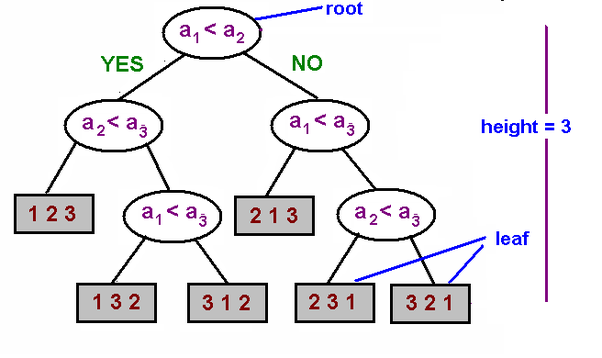
\includegraphics[width=\textwidth]{img/decision-tree.png}
    \caption{Albero di decisione per l'array $A[1,2,3]$}
\end{figure}

\paragraph{Osservazioni}
\begin{itemize}
	\item $ \text{Altezza dell'albero di decisione} = \text{limite inferiore per caso pessimo}$
	\begin{align*}
	    \text{per }& \text{IS} \ \quad n^2 \\
	    \text{per }& \text{MS} \quad n \log n
	\end{align*}
	\item Ogni foglia ha una sola permutazione. Ogni permutazione compare (almeno) in una foglia.
\end{itemize}

\emph{In generale}, le foglie contengono \underline{tutte} le permutazioni.
$$ \text{\# foglie} \geq \text{\# permutazioni} = n! \qquad ( \text{\# foglie} \leq 2^h)$$
\begin{align*}
    h & \geq \log_2 n! \\
    & \geq \log_2 \left( n(n-1)(n-2) \dots \frac{n}{2}\right) \\
    & \geq \log_2 \left( \frac{n}{2}\left(\frac{n}{2}-1\right)\left(\frac{n}{2}-2\right) \dots \frac{n}{2}\right) \\
    & \geq \log_2 \left( \frac{n}{2} \right)^{(\frac{n}{2})} 
        = \frac{n}{2} \left( \log_2 n - \log_22\right)
        = \frac{n}{2} (\log_2 n - 1) = \Theta (n \log n)
\end{align*}
Inoltre,
\begin{itemize}
	\item $ \text{\# operazioni} \geq h = \Omega (n \log n)$
	\item $ \texttt{Heapsort, MergeSort } O(n \log n))$ 
\end{itemize}
$\Rightarrow \text{ordinamento (bastato su confronti) } \Theta (n \log n)$

\subsection{Counting Sort}
Esistono degli algoritmi di ordinamento che, in certe condizioni e per certi input, permettono
di ordinare in tempo lineare $\Omega (n)$
\bigskip

Assumo
\begin{itemize}[label=$-$]
    \item interi;
    \item in $[0,k]$
\end{itemize}

\begin{itemize}[label=]
    \item \texttt{Input}: $A[1\twodots n]$ con $A[j] \in [0,k] \quad \forall 1 \leq j \leq n$;
    \item \texttt{Output}: $B[1\twodots n]$ permutazione ordinata di $A$;
    \item \texttt{Supporto}: $C[0\twodots k]$.
\end{itemize}

\begin{codebox}
\Procname{$\proc{Counting-Sort}(A,B,k)$}
\li $C[0\twodots k] \leftarrow 0$
\li \For $j \gets 1$ \To $\attrib{A}{length}$
\zi \Do
		\Comment $C[x] =$ \verb|#| elementi in $A$ con valore $x$
\li		$C[A[j]] \gets C[A[j]] + 1$ 
    \End
\li \For $i \gets 1$ \To $k$
\zi \Do
        \Comment $C[x] =$ \verb|#| elementi in $A$ con valore $\leq x$
\li     $C[i] \gets C[i-1] + C[i]$ 
    \End
\li \For $j \gets \attrib{A}{length}$ \Downto $1$
\li \Do
        $B[C[A[j]]] \gets A[j]$
\li     $C[A[j]] \gets C[A[j]] - 1$
    \End
\end{codebox} 

\paragraph{Complessità} 
\begin{align*}
    C[0,k] \leftarrow 0 && \Theta(k) \\
    \text{\texttt{for j=1}} \dots && \Theta(n) \\
    \text{\texttt{for i=1}} \dots && \Theta(k) \\
    \text{\texttt{for j=A.length}} \dots && \Theta(n)
\end{align*}
$$\text{Somma } \Theta(n+k) \text{ con } k = \Theta(1) \Rightarrow \Theta(n)$$

\paragraph{Problema di memoria} Il problema di \texttt{CountingSort} è la memoria. 
Infatti, al crescere di $k$, la memoria richiesta per allocare \texttt{C} cresce esponenzialmente.
\begin{center}
    \begin{tabular}{|l|l|}
        \hline
        Dimensione $k$ & Memoria occupata da \texttt{C[]} \\
        \hline
        1 Byte $= 8$ bit & $2^8 \text{Bytes} = 256 \text{Bytes}$ \\
        2 Bytes $= 16$ bit & $2^{16} \text{Byte} \cdot 2 \text{Bytes} = 256 \text{Megabytes}$ \\
        8 Bytes $= 64$ bit & $2^{64} \text{Byte} \cdot 8 \text{Bytes} = 512 \text{Terabytes}$ \\
        \hline
    \end{tabular}
\end{center}

\subsubsection{Proprietà di Stabilità}
Dato $A[1 \twodots n]$ in input, se $A[i] \leq A[j]$ con $i \leq j$, allora nell'output $A[i]$ e $A[j]$ sono nello stesso ordine relativo.
\bigskip

Algoritmi stabili:
\begin{itemize}
	\item \texttt{MergeSort}
	\item \texttt{InsertionSort}
\end{itemize}
\bigskip

Algoritmi non stabili:
\begin{itemize}
	\item \texttt{CountingSort}
	\item \texttt{Quicksort}
	\item \texttt{Heapsort}
\end{itemize}
\subsection{Radix Sort}
Il \href{https://en.wikipedia.org/wiki/Radix_sort}{Radix Sort} è un algoritmo di ordinamento in tempo
lineare $O(n)$, come \texttt{CountingSort}, che risolve i problemi di memoria di quest'ultimo.

L'idea è quella di ordinare cifra per cifra, dalla cifra meno significativa alla più significativa con un 
algoritmo \emph{stabile}.
\begin{align*}
	\text{(iniziale)} && \text{(terza cifra)} && \text{(seconda cifra)} && \text{(prima cifra)} \\
	329 && 720 && 720 && 329 \\
	457 && 355 && 329 && 355 \\
	657 && 436 && 436 && 436 \\
	839 && 457 && 839 && 457 \\
	436 && 657 && 355 && 657 \\
	720 && 329 && 457 && 720 \\
	355 && 839 && 657 && 839 \\
\end{align*}

\texttt{Input}: \texttt{A[1$\twodots$n]} con \texttt{A[i]} di $d$ cifre e base $b$,
\texttt{A[i]}$= a_d a_{d-1}\dots a_1$.

\begin{codebox}
\Procname{\proc{RadixSort}$(A,d)$}
\li \For $j \gets 1$ \To $d$
\li \Then
		$\text{ordina $A$ rispetto alla cifra $j$}$
		\Comment $A^j[i] = a_j a_{j-1} \dots a_1$
\zi 	$\text{con}$ \proc{CountingSort}
		\Comment $A^{j-1} ordinato$
	\End
\end{codebox}

\paragraph{Correttezza di RadixSort(A, d)}
\begin{itemize}
	\item \textbf{Inizializzazione}: ok;
	\item \textbf{Mantenimento}: se $A^{j-1}$ è ordinato e ordino rispetto alla $j$-esima cifra con
	un algoritmo stabile, allora $A^j$ è ordinato.
	$$i < i' \Rightarrow A^j[i] \leq A^j[i']$$
	\begin{align*}
		\text{Siano } & A^j[i] = a_j a_{j-1} \dots a_1 \\
		& A^j[i'] = a'_j a'_{j-1} \dots a_1
	\end{align*}
	
	Posso distinguere due casi:
	\begin{enumerate}
		\item \begin{align*}
			a_j \neq a'_j & \Rightarrow a_j < a'_j \\
			& \Rightarrow A^j[i] < A^j[i']
		\end{align*}
		\item \begin{align*}
			a_j = a'_j & \Rightarrow A^j[i] \leq A^j[i'] \qquad \text{(stabilità)}\\
			& \Rightarrow A^j[i] = a_j A^j[i] \leq \\
			& \leq A^j[i'] = a'_j A^{j-1}[i']
		\end{align*}
	\end{enumerate}
\end{itemize}

\paragraph{Complessità} 
\begin{gather*}
	d \text{ volte \texttt{CountingSort} } \; \Theta(n+b) \Rightarrow \Theta\big(d(n+b)\big) = \Theta(n) \\
	\text{con } d \text{ cifre } = \Theta(1), \text{ base } b = \Theta(n) 
\end{gather*}
\begin{align*}
	m \text{ bit, } r \text{ bit per cifra, } \frac{m}{r} \text{ cifre, base } 2^r \\
	\Theta( \frac{m}{r} (m + 2^r)) & = && r = \log_2 n \\
	& = \Theta( \frac{m}{ \log n} (n + 2^{ \log n} )) \\
	& = \Theta( \frac{m}{ \log n} n) && m = O( \log n) \\
	& 	= \Theta(n)
\end{align*}

\section{Tabelle Hash}
\begin{gather*}
	U \text{ universo delle chiavi} \\
	U = \{ 0, 1, \dots, \abs{U} - 1 \} \\
	T[0 \twodots \abs{U} - 1] \text{ tabella hash}	
\end{gather*}
\[ T[k] \text{ contiene} \quad
	\begin{cases}
		\text{elemento } x \text{ con } x.key = k & \text{se c'è} \\
		\const{nil} & \text{altrimenti}
	\end{cases}
\]

\begin{codebox}
\Procname{\proc{Insert}$(T,x)$}
\li $T[\attrib{x}{\id{key}}] \gets x$
	\Comment $\Theta(1)$
\end{codebox}
\begin{codebox}
\Procname{\proc{Delete}$(T,x)$}
\li $T[\attrib{x}{\id{key}}] \gets nil$
	\Comment $\Theta(1)$
\end{codebox}
\begin{codebox}
\Procname{\proc{Search}$(k)$}
\li \Return $T[k]$
	\Comment $\Theta(1)$
\end{codebox}

\paragraph{Problema} e.g. consideriamo che la \emph{key} sia di 8 caratteri (e 8 bit per rappresentare
un carattere). Risulta molto costosa in termini di memoria la tabella hash.
\begin{gather*}
	2^8 \dots 2^8 \\
	(2^8)^8 = 2^{64} \cong 10^{19}
\end{gather*}

\paragraph{Idea} 
\begin{gather*}
	U = \{ 0, 1, \dots , \abs{U} - 1 \} \\
	T[0 \dots m-1] \qquad m << \abs{U}
\end{gather*}
La ``traduzione'' per ottenere $x.key$ da $x$ cosa comporta?
\begin{gather*}
	h \colon U \to \{ 0, 1, \dots , m-1 \} \text{ funzione di \emph{hashing}} \\
	n = \text{\# elementi memorizzati nella tabella } T \\
	m = \text{\# celle}
\end{gather*}
Se $n > m$, esisteranno $x_1, x_2 : h(x_1.key) = h(x_2.key) \Rightarrow$ conflitto \par
\bigskip 
Abbiamo \emph{due soluzioni}:
\begin{enumerate}
	\item \textbf{Chaining} (\ref{hash:chaining});
	\item \textbf{Open Addressing} (\ref{hash:openaddessing}).
\end{enumerate}
\subsection{Chaining}\label{hash:chaining}
Il \emph{Chaining} propone come soluzione quella di mettere sulla tabella liste dinamiche
di elementi, invece che singoli elementi, in modo che in caso si incorra in una cella
già occupata dopo un \emph{hashing}, l'elemento venga inserito in coda (o in testa) alla
lista.

\paragraph{Idea} \texttt{T[i]} $=$ lista elementi $x$ tali che $h(x.key) = i$

\begin{codebox}
\Procname{\proc{Insert}$(T,x)$}
\li	$\text{Inserisci $x$ nella lista } T[h(x.key)]$
	\Comment $O(1)$
\end{codebox}
\begin{codebox}
\Procname{\proc{Delete}$(T,x)$}
\li	$\text{Delete $x$ from } T[h(x.key)]$
	\Comment $O(1)$
\end{codebox}
\begin{codebox}
\Procname{\proc{Search}$(T,k)$}
\li	$\text{Cerca in } T[h(k)] \text{ un elemento } x \text{ tale che } \attrib{x}{\id{key}} = k$ 
	\Comment $O(n)$
\end{codebox}
\texttt{Search} ha una complessità di $O(n)$, e questo è inaccettabile.
\begin{gather*}
	n = \# \text{elementi inseriti} \\
	m = \text{dimensione di } T \\
	\alpha = \frac{n}{m} \quad \text{fattore di carico} \\
	\alpha \text{ può essere }<, \ = \text{ oppure } > \text{ di } 1
\end{gather*}

\subsubsection{Hashing uniforme semplice}
Ogni elemento di \emph{input} è ``mandato'' da $h$ con la stessa probabilità $\left( \frac{1}{m} \right)$
in una delle $m$ celle.

\paragraph{Caso medio} $\Theta(1 + \alpha)$, 1 è l'accesso alla tabella.\par
Consideriamo $n_1,n_2,\dots,n_{m-1}$ la lunghezza delle $m$ liste. La lunghezza attesa
di una lista è:
$$E[n_j] = \displaystyle\sum_{i = 1}^{n} \frac{1}{m} \cdot 1 = \frac{n}{m} = \alpha$$

\paragraph{Ricerca di una chiave} La chiave può essere:
\begin{itemize}
	\item \emph{Assente}. \texttt{Search(k)}, \texttt{k} non c'è.
	\begin{itemize}
		\item Calcolo \texttt{h(k)} $\rightarrow$ ($\Theta(1)$);
		\item Accedo a \texttt{T[h(k)] = j} $\rightarrow$ ($\Theta(1)$);
		\item Scorro $n_j$ elementi ($n_j = \alpha$) $\rightarrow (\Theta(\alpha)$).  
	\end{itemize}
	Nel complesso, ho $\Theta(1+\alpha)$

	\item \emph{Presente}. \texttt{Search(k)}, \texttt{k} presente.
	\begin{itemize}
		\item \texttt{h(k)} e \texttt{T[h(k)]}\par
			$$\text{Se } x_1, x_2,\dots x_n \text{ sono gli elementi inseriti}$$
		Costo della ricerca di $x_i$:
		\begin{align*}
			& 1 + \# elem \quad x_j : j > 1, \ h(x_i.key) = h(x_j.key) \\
			& = 1 + \displaystyle\sum_{j=i+1}^n \left(prob \ h(x_i.key) = h(x_j.key)\right) \\
			& = 1 + \displaystyle\sum_{j=i+1}^n \frac{1}{m} = 1 + \frac{n-i}{m}
		\end{align*}
		\begin{align*}
			& \frac{1}{n} \displaystyle\sum_{i=1}^n \left( 1 + \frac{n-i}{m} \right) \\
			& = \frac{1}{n} \left( n + \displaystyle\sum_{i=1}^n \frac{n-i}{m} \right) 
				= \frac{1}{n} \left( n + \frac{1}{m} \displaystyle\sum_{z=0}^{n-1} z \right) \\
			& = 1 + \frac{1}{m \cdot n} \cdot \frac{n(n-1)}{2} = 1 + \frac{n}{2m} - \frac{1}{2m} \cdot \left(\frac{n}{n} \right) \\
			& \hspace{5cm} \left(\frac{n}{m} = \alpha\right) \\
			& = 1 + \frac{\alpha}{2} - \frac{\alpha}{2n} = \Theta(1+\alpha)
		\end{align*}

		\begin{gather*}
			\text{Se } n \leq c \cdot m \text{ per qualche costante positiva } c \text{ allora}\\ 
			\alpha \leq c \Rightarrow \Theta(1)
		\end{gather*}
	\end{itemize}
	\item $h : U \implies \{ 0,1,\dots,m-1 \} \Rightarrow h(x) = 0$
\end{itemize}

\subsubsection{Funzioni Hash} Una \emph{funzione hash} deve soddisfare la proprietà di
\emph{hashing uniforme}, ossia 
\begin{quote}
	``Ogni chiave ha la stesso probabilità $\frac{1}{m}$ di essere mandata in una
	qualsiasi delle $m$ celle, indipendentemente dalle chiavi inserite precedentemente.''
\end{quote} 
Consideriamo:
\begin{itemize}
	\item $x \in [0,1)$ ($0 \leq x < 1$), $x$ chiave, estratta in modo indipendente dalla distribuzione
	uniforme (\underline{non realistica}).
	\item Allora $h(x) = \floor{mx}$ soddisfa la proprietà di \emph{hashing uniforme}.
\end{itemize} 

L'ipotesi di hash uniforme semplice dipende dalle probabilità con cui vengono estratti gli elementi da
inserire; probabilità che in genere non sono note.
Le funzioni hash che descriveremo assumono che le chiavi siano degli interi non negativi.

\paragraph{Metodo della divisione} 
$$U = \{ 0, 1, \twodots, \abs{\cup} - 1 \}$$
$$h(k) = k \mod n$$
\begin{itemize}
	\item $m = 2^p$ caso pessimo;
	\item $m = 2^p - 1$ caso non buono. $2^p$ cifre base.
\end{itemize}
La soluzione migliore è quella di scegliere chiavi lontane dalle potenze di 2, meglio
ancora se numeri primi.

\paragraph{Metodo della moltiplicazione}
$$k \in U$$
$$0 < A < 1 \text{ fissato}$$
$$h(k) = m(k A \mod 1) \qquad \text{Miglior } A : \frac{\sqrt{5}-1}{2}$$
\begin{align*}
	m & = 2^p \quad w = \# \text{bit parola} \\
	A & = \frac{q}{2^w} \quad 0 < q < 2 \\
	& m(k A \mod 1) \\
	& = m \left( k \frac{q}{2^w} \mod 1 \right) && (\text{\emph{shift} di $w$ bit, prendo la parte decimale} \\
	& && k a \mod 1 \text{ e la moltiplico per } m = 2^p) 
\end{align*}

\subsubsection{Hashing Universale} 
Per avere una distribuzione più uniforme delle chiavi nelle liste e non dipendente dall'input,
possiamo usare la \emph{randomizzazione}. \par
Insieme $H$ di funzioni di hash. Scelgo randomicamente da $H$. \par
Sotto certe ipotesi ottengo per \texttt{Search}:
$$\Theta(1 + \alpha)$$

\paragraph{Def (Hashing universale)} $\forall k_1,k_2 \in U \ k_1 \neq k_2$
\begin{gather*}
	\left| \left\{ h \in H : h(k_1) = h(k_2) \right\} \right| \leq \frac{|H|}{m} \\
	\frac{\left| \left\{ h \in H : h(k_1) = h(k_2) \right\} \right|}{|H|} \leq \frac{1}{m}
\end{gather*}

Con il \emph{chaining}, $H$ è universale per ogni $k \in U, \ j = h(k)$
\[ \text{Costo medio } \Theta(1+\alpha)
	\begin{cases}
		k \text{ non è in } T \rightarrow E[n_j] \leq \alpha \\
		k \text{ è in } T \rightarrow E[n_j] \leq 1 + \alpha
	\end{cases}
\]


% 05/04/2018
\section{Lezione 13}

\subsection{Open Addressing} \label{hash:openaddessing}

$h(k,i)$: $k$ è la chiave, $i$ è il tentativo.\par
Provo con $h(k,0)$: se capito in una cella occupata, provo con $h(k,1)$, poi $h(k,2)$
e così via, fino a che non trovo una cella libera.

Per esplorare tutta la tabella:
$$h(k,0), h(k,1), \dots, h(k,m-1)$$
che è una permutazione di 
$$0,1,\dots,m-1$$

\begin{codebox}
\Procname{\proc{Insert}$(T,x)$}
\li $i \gets 0$
\li \Repeat
\li     $j \gets h(\attrib{x}{\id{key}},i)$
\li     \If $(T[j] = \const{nil}) \kw{ or } (T[j] = \const{deleted})$ 
        \Comment posizione libera
\li         \Then
                $T[j] \gets x$
\li             \Return $j$
            \End
\li     $i \gets i + 1$
\li \Until $i = m$
\li \kw{error}
\end{codebox}
\begin{codebox}
\Procname{$\proc{Search}(T,k)$}
\li $i \gets 0$
\li \Repeat 
\li     $j \gets h(k,i)$
\li     \If $\attrib{T[j]}{key} = k$
\li     \Then
            \Return $j$
        \End
\li     $i \gets i + 1$
\li \Until $(i = m)$ \Or $(T[j] = \const{nil})$
\li \Return \const{not found}
\end{codebox}
\begin{codebox}
\Procname{$\proc{Delete}(T,j)$}
\li $T[j] = \const{deleted}$
\end{codebox}
L'\emph{Open Addressing} risulta una soluzione inefficiente in caso
avvengano molte cancellazioni.

\subsubsection{Hashing uniforme}

Per ogni elemento di input, tutte ($m!$) le sequenze di ispezione
sono equiprobabili.

\subsubsection{Funzioni di Hash}
\begin{enumerate}
    \item \textbf{Ispezione lineare}. Sia $h'(k)$ funzione di hash ``ordinaria''. Se 
        ricado in una cella occupata, mi sposto su quella immediatamente successiva.
        $$h(k,i) = (h'(k)+i) \mod m$$
        Caratteristiche:
        \begin{itemize}
            \item è semplice;
            \item poche permutazioni ($m$ dipende solo da $h'(k)$);
            \item causa addensamenti di celle occupate (\emph{addensamento primario}).
        \end{itemize}
    \item \textbf{Ispezione quadratica}. Fisso $h'(k)$.
    $$h(k,i) = h'(k) + c_1i + c_2i^2 \qquad c_2 \neq 0$$

    \begin{codebox}
        \Procname{Inserimento di $k$}
        \zi $j \gets h'(k)$
        \zi $i \gets 0$
        \zi \While $(i < m)$ \kw{and} $(T[j] \neq \const{nil}/\const{deleted})$
        \zi \Do
                $i \gets i + 1$
        \zi     $j \gets (j + 1) \mod n$
            \End
    \end{codebox}

    \begin{description}
        \item[$(i=0) \quad$] $j = h'(k)$
        \item[$(i=1) \quad$] $j = (h'(k)+1) /mod m$
        \item[$\vdots$] 
        \item[$(i=l) \quad$] 
        \begin{align*}
            j & = \left( h'(k) + \displaystyle\sum_{i=1}^{l}i \right) \mod m \\
            & = \left( h'(k) + \frac{l(l+1)}{2} \right) \mod m \\
            & = \left( h'(k) + \frac{1}{2}l + \frac{1}{2}l^2 \right) \mod m \\
            & m = 2^p \text{ permutazione}
        \end{align*}
    \end{description}
    \item \textbf{Doppio Hash}. Fisso $h_1(k)$, $h_2(k)$
    $$h(k,i) = (h_1(k) + i \cdot h_2(k)) \mod m$$
    \emph{Osservazioni}:
    \begin{itemize}
        \item I salti sono di dimensione $h_2(k)$ all'incrementare di $i$; 
        \item Ci sono $m^2$ sequenze di ispezione;
        \item $h_2(k)$ e $m$ primi tra loro $ \quad (MCD = 1)$;
        \item $i, i<m \quad h(k,i) = h(k,i') \Rightarrow i = i' \ \quad (\text{\emph{iniettività}})$
        $$h(k, \verb|_|) : \{ 0, \_, m-1 \} \rightarrow \{ 0,\verb|_|, m-1 \}$$
        $$\text{\emph{iniettiva}} \Rightarrow \text{\emph{biiettiva}}$$
        \begin{gather*}
            h(k,i) = h(k,i') \\
            (h_1(k) + ih_2(k)) \mod m = (h_1(k) + i'h_2(k)) \mod m \\
            ((i - i')h_2(k)) \mod m = (i h_2(k) - i'h_2(k)) \mod m = 0 \\
            (i - i') \mod m = 0 \\
            i \geq i' \quad i - i' < m \\ 
            \Rightarrow i - i' = 0 \\
            \Rightarrow i = i'
        \end{gather*}
        Scelgo $m = 2^p, \ h_2(k) = 1 + 2h_2'(k)$, $h_2'(k)$ qualunque.\par
        \emph{es.} $h_2(k) = 1 + k \mod m' \quad$ con $m' < m$
    \end{itemize}
    \end{enumerate}

\paragraph{Costo?}
Il costo della \texttt{Search} con \emph{hashing uniforme} si può riassumere come segue.
$$0 \leq \alpha = \frac{n}{m} \leq 1$$

\paragraph{Ricerca di una chiave non presente}
\begin{enumerate}[label=(\alph*)]
    \item $\frac{1}{1-\alpha} \quad$ se $\alpha < 1$
    \item $m \quad$ se $\alpha = 1$ 
\end{enumerate}

\subparagraph{Probabilità di ispezionare la i-esima cella}
\begin{center}
    \begin{tabular}{c|l}
        \textbf{cella} & \textbf{probabilità} \\
        \hline
        $i = 0$ & 1 \\
        $i = 1$ & prob. cella 0 occupata: $\frac{n}{m}$ \\
        $i = 2$ & prob. cella 1 occupata: $\frac{n}{m} \cdot \frac{n-1}{m-1}$ \\
        $\dots$ \\
        $i$ & $\frac{n}{m} \cdot \frac{n-1}{m-1} \dots \frac{n-i+1}{m-i+1} \leq \alpha \cdot \alpha \dots \alpha = \alpha^i$
    \end{tabular}
\end{center}

Valore atteso per \#celle ispezionate
$$1 + \alpha + \alpha^2 + \dots + \alpha^{i-1} + \dots + \alpha^{m-1}$$

\begin{enumerate}[label=(\alph*)]
    \item $\alpha < 1 \Rightarrow \frac{1 - \alpha^m}{1 - \alpha} \leq \frac{1}{1-\alpha}$ 
    \item $m$ 
\end{enumerate}

\paragraph{Ricerca di una chiave presente}
\begin{enumerate}[label=(\alph*)]
    \item $\frac{1}{\alpha} \log \left( \frac{1}{1-\alpha} \right) \quad \alpha < 1$
    \item $1 + \log m \quad \alpha = 1$
\end{enumerate}

Finora, ho inserito $x_0,x_1,\dots, x_i,\dots,x_n$.
\begin{gather*}
    \text{costo \texttt{Search} chiave $x_i$ presente} \\
    = \text{costo \texttt{Search} chiave $x_i$ assente} \\
    \text{in }  x_0,\dots,x_{i-1} \quad \frac{1}{1-\alpha_i}, \ \alpha_i = \frac{i}{m}
\end{gather*}

Numero medio:
\begin{align*}
    & \frac{1}{n} \displaystyle\sum_{i=0}^{n-1}\frac{1}{1-\alpha_i} 
        = \frac{1}{n} \displaystyle\sum_{i=0}^{n-1} \frac{m}{m-i} 
        = \frac{m}{n}\displaystyle\sum_{i=0}^{n-1} \frac{1}{m-i} \qquad \left(\frac{m}{n} = \frac{1}{\alpha} \right)\\
    & = \frac{1}{\alpha} \displaystyle\sum_{l=m-n+1}^{m}\frac{1}{l} \qquad (m-i \rightarrow m-n+1) 
\end{align*}

\begin{itemize}
    \item Se $\alpha < 1$ %SISTEMARE, <= di cosa?
    \begin{align*}
        & \leq \frac{1}{\alpha} \int_{n-m}^{m}\frac{1}{x} \mathrm{d}x \\ 
        & = \frac{1}{\alpha}\left( \log m - \log (m-n) \right) = \frac{1}{\alpha}\left( \log \frac{m}{m-n} \right) \\
        & = \frac{1}{\alpha} \log \frac{1}{\frac{m-n}{m}} \\ 
        & = \frac{1}{\alpha} \log \left( \frac{1}{1-\left( \frac{n}{m} \right)} \right)
            = \frac{1}{\alpha} \log \left( \frac{1}{1-\alpha } \right)
    \end{align*}

    \item Se $\alpha = 1$
    \begin{align*}
        \displaystyle\sum_{l = 1}^{m} \frac{1}{l} & = 1 + \displaystyle\sum_{l=2}^m \frac{1}{l} 
            \leq \int_1^m \frac{1}{x} \mathrm{d}x \\
        & = 1 + \left( \log m - \log 1 \right) = 1 + \log m
    \end{align*}
\end{itemize}

Confrontiamo le complessità dei due casi.

\begin{center}
    \begin{tabular}{l|l|l}
        $\alpha$ & $\frac{l}{1-\alpha}$ & $\frac{1}{\alpha} \log \left( \frac{1}{1-\alpha} \right)$ \\
        \hline
        $\alpha = 0.3$  & 1.43 & 1.19 \\
        $\alpha = 0.5$  & 2.00 & 1.39 \\
        $\alpha = 0.7$  & 3.33 & 1.72 \\
        $\alpha = 0.9$  & 10 & 2.56 \\
        $\alpha = 0.99$ & 100 & 4.65         
    \end{tabular}
\end{center}
\section{Lezione 14}

\subsection{Max Heap con coda dinamica}
Implementiamo un \texttt{Max Heap}, solo che è implementato con una
coda dinamica invece che con un normale array.

Ogni \emph{nodo} $x$ ha 3 campi dato:
\begin{itemize}[noitemsep]
    \item \texttt{x.left};
    \item \texttt{x.right};
    \item \texttt{x.p}.
\end{itemize}

$H$ è lo \emph{heap} ($\const{nil}$ se vuoto):
\begin{itemize}[noitemsep]
    \item \texttt{H.root};
    \item \texttt{H.size}.
\end{itemize}

Abbiamo \texttt{MaxHeapify} e \texttt{MaxHeapifyUp} invariate.

\begin{codebox}
\Procname{\proc{Insert}$(H, \id{node})$}
\li \If $\attrib{H}{size} = 0$
\li     \Then
            $\attrib{\id{node}}{p} \gets \const{nil}$
\li         $\attrib{H}{root} \gets \id{node}$
\li         $\attrib{H}{size} = 1$
\li     \Else
\li         $x \gets root$
\li         $\attrib{H}{size} \gets \attrib{H}{size} + 1$
\li         $p \gets \proc{bitvector}(\attrib{H}{size})$
            \Comment $p$ letto come vettore di bit
\li         $k \gets \# \text{bit di p più significativo a 1}$
\li         \For $i \gets k-1$ \kw{down} \To $1$
\li             \Do 
                    \If $p[i] = 0$
\li                     \Then
                            $x \gets \attrib{x}{left}$
\li                     \Else 
\li                         $x \gets \attrib{x}{right}$
                    \End
            \End
\li         \If $p[0] = 0$
\li             \Then
                    $\attrib{x}{left} \gets \id{node}$
\li             \Else
\li                 $\attrib{x}{right} \gets \id{node}$
            \End
    \End
\li $\attrib{\id{node}}{left} \gets \attrib{\id{node}}{right} \gets \const{nil}$
\li $\proc{MaxHeapifyUp}(H, \id{node})$
\end{codebox} 

Raccolta esercizi della lezione: \ref{exs:6-4-2018}.
\subsection{Red-Black Trees}

I \emph{Red-Black Trees} sono ABR i cui nodi hanno un campo \emph{colore} $x.col$, che può essere:
\begin{itemize}[noitemsep]
    \item \textbf{R} per il rosso;
    \item \textbf{B} per il nero.
\end{itemize}

\paragraph{Accorgimento} $\const{nil}$ sarà in realtà un nodo,
$T.nil$, con $T.nil.col = B$.

\paragraph{Caratteristiche} \emph{RB-tree} è in realtà un ABR tale che:
\begin{enumerate}[label=($\arabic*$)]
    \item Ogni nodo $x$ ha $x.col \in \{R,B\}$; \label{rbtree:1}
    \item La radice $root$ è $B$; \label{rbtree:2}
    \item Le foglie ($T.nil$) sono $B$; \label{rbtree:3}
    \item Se $x$ è $R$, i figli sono $B$; \label{rbtree:4}
    \item Per ogni nodo $x$, ogni cammino da $x$ a una qualsiasi delle foglie
    ha lo stesso numero di nodi $B$ (calcolato con $bh(x)$). \label{rbtree:5}
\end{enumerate} 

\begin{figure}[hbt]
    \centering
    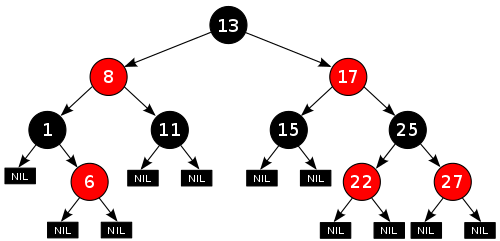
\includegraphics[width=\textwidth]{img/rb-tree-ex.png}
    \caption{Esempio di un RB-tree.}
\end{figure}
\pagebreak

È possibile notare che: 
\begin{itemize}
    \item In caso non ci fossero nodi rossi, avremo un albero
    perfettamente bilanciato;
    \item In ogni cammino, il \verb|#| di nodi \textbf{B} è almeno la
    metà del \verb|#| dei nodi \textbf{R}
\end{itemize}

\paragraph{Osservazione} Se $T$ è un \emph{RB-tree} con $n$ nodi interni ($\neq \const{nil}$)
e $h$ altezza, allora vale
$$h \leq 2 \log (n + 1)$$

\subparagraph{Dimostrazione} Consideriamo 
$$n_x \geq 2^{bh(x)} - 1$$
La dimostrazione è per induzione su $h_x$ (altezza del sotto-albero radicato in $x$).

\begin{description}
    \item[$(h_x = 1)$] Allora ho solo 
    $T.nil \Rightarrow n_x = 0 = 2^0 - 1 \qquad (2^0 \text{ con } 0 = bh(x))$
    \item[$(h_x > 1)$] Consideriamo $x$ radice. $x$ ha due figli, $x_1$ e $x_2$.\par
    Sicuramente vale $h_1,h_2 < h$. Per ipotesi induttiva, valgono:
    $$n_{x_1} \geq 2^{bh(x_1)} - 1$$
    $$n_{x_2} \geq 2^{bh(x_2)} - 1$$
    \begin{align*}
        n_x & = n_{x_1} + n_{x_2} + 1 \\
        & \geq 2^{bh(x_1)} + 2^{bh(x_2)} - 1 \\
        & \geq 2 \cdot 2^{bh(x)-1} - 1 = 2^{bh(x)} - 1 \\
        & \qquad (\text{valgono } bh(x_1) \geq bh(x)-1, \ bh(x_2) \geq bh(x)-1) \\
        \text{Comples}&\text{sivamente}\\
        n & = n_{root} \geq 2^{bh(root)} - 1
    \end{align*}
    Essendo $bh(root) \geq \frac{h}{2}$, posso ottenere
    \begin{align*}
        n_{root} & \geq 2^{bh(root)} - 1 \\
        & 2^{\frac{h}{2}} - 1 \\
        \Rightarrow \ & 2^{\frac{h}{2}} \leq n + 1 \\
        & \frac{h}{2} \leq \log_2(n+1) \Rightarrow h \leq 2 \log_2(n+1) 
    \end{align*}
\end{description}

\subsubsection{Complessità algoritmi RB-Trees}
\texttt{Search, Succ, Min, Pred, Max} hanno un costo di $O(h) = O(\log n)$

%2/5/2018

\subsubsection{RB-Insert e RB-Delete}
A differenza di quelle citate precedentemente, che risultano semplici
sia come complessità asintotica che come implementazione, Bisogna porre 
particolare attenzione a queste due procedure: \texttt{RB-Insert} e \texttt{RB-Delete}.

Per ovviare a ciò, posso utilizzare le \emph{rotazioni}. Consideriamo il seguente albero,
in cui $x$ e $y$ sono nodi normali, mentre $\alpha, \ \beta$ e $\gamma$ sono sotto-alberi
(il colore dei nodi non ha importanza ai fini della procedura che andremo a 
vedere)\footnote{Di conseguenza, applicandola a un \emph{RB-tree}, gli assiomi di validità potrebbero venire violati.}:
\begin{center}
	\begin{tikzpicture}
	\Tree
	[.$x$     
		[.$\alpha$
		]
		[.$y$ 
            [.$\beta$ 
                \edge[blank]; \node[blank]{};
                \edge[blank]; \node[blank]{};
            ]
			[.$\gamma$ 
                \edge[blank]; \node[blank]{};
                \edge[blank]; \node[blank]{};
            ]
		]
	]
	\end{tikzpicture}
\end{center}
Applichiamo la procedura \texttt{Left(T,x)}, ottenendo:
\begin{center}
	\begin{tikzpicture}
	\Tree
	[.$y$
        [.$x$
            [.$\alpha$ 
                \edge[blank]; \node[blank]{};
                \edge[blank]; \node[blank]{};
            ]
            [.$\beta$ 
                \edge[blank]; \node[blank]{};
                \edge[blank]; \node[blank]{};
            ]
		]
		[.$\gamma$ ]
	]
	\end{tikzpicture}
\end{center}

\paragraph{Osservazione} La \emph{visita simmetrica} è identica per i due alberi:
$$\alpha \rightarrow x \rightarrow \beta \rightarrow y \rightarrow \gamma$$

\begin{codebox}
\Procname{\proc{Left}$(T,x)$}
\li $\attrib{x}{right} \gets \attrib{y}{left}$
\li $\attrib{\attrib{x}{right}}{p} \gets x$
\li $\attrib{y}{left} \gets x$
\li $\attrib{x}{p} \gets y$
\li $\proc{Transplant}(T,x,y)$
\end{codebox}

\paragraph{RB-Insert(T, z)} Voglio inserire $z$ nell'albero $T$.
L'idea è quella di porre $z.col = \const{red}$ poichè meno insidioso\footnote{Andando a modificare il numero di nodi neri, cambia l'altezza nera, e la cosa è difficile da sistemare.}.
\begin{itemize}
    \item Se violo \ref{rbtree:2} $\Rightarrow z.col = \const{black}$;
    \item Se violo \ref{rbtree:4}:
    \begin{itemize}
        \item Risolvo localmente;
        \item Sposto verso l'alto il problema.
    \end{itemize}
\end{itemize}

Abbiamo due \emph{macrocasi}. $z.p$ è figlio sinistro, oppure destro. Noi analizzeremo solo il primo: \textbf{z.p figlio sinistro}.
\begin{center}
	\begin{tikzpicture}
	\Tree
	[.$\boldsymbol{z.p.p}$
        [.$\boldsymbol{\color{red} z.p}$
            [.$\boldsymbol{\color{red} z}$
            ]
		]
		[.$y$ 
        \edge[blank]; \node[blank]{};
        \edge[blank]; \node[blank]{};
        ]
    ]
	\end{tikzpicture}
\end{center}
\clearpage
Abbiamo due possibilità per $y$\footnote{I nodi con testo in rosso sono $\const{red}$, %
quelli in grassetto sono $\const{black}$, e quelli normali possono essere sia rossi che neri.}:
\begin{enumerate}
    \item $y.col = \const{red}$. Ci è sufficiente invertire il colore di $z.p.p$ con quello dei figli.
    \begin{center}
        \begin{tikzpicture}
        \Tree
        [.$\boldsymbol{\color{red} z.p.p}$
            [.$\boldsymbol{z.p}$
                [.$\boldsymbol{\color{red} z}$
                ]
            ]
            [.$\boldsymbol{y}$ 
            \edge[blank]; \node[blank]{};
            \edge[blank]; \node[blank]{};
            ]
        ]
        \end{tikzpicture}
    \end{center}
    In questo modo, risolviamo localmente e rimandiamo il problema in alto.
    \item $y.col = \const{black}$. Possiamo distinguere due sottocasi.
    \begin{enumerate}[label=($2.\arabic*$)]
        \item $z$ figlio destro. \label{rbinsert:2.1}
        \begin{center}
            \begin{tikzpicture}
            \Tree
            [.$\boldsymbol{z.p.p}$
                [.$\boldsymbol{\color{red} z.p}$
                    \edge[blank]; \node[blank]{};
                    [.$\boldsymbol{\color{red} z}$
                    ]
                ]
                [.$\boldsymbol{y}$ 
                \edge[blank]; \node[blank]{};
                \edge[blank]; \node[blank]{};
                ]
            ]
            \end{tikzpicture}
        \end{center}
        Voglio finire nel caso \ref{rbinsert:2.2}. Applico \texttt{Left(T,z.p)}, ottenendo:
        \begin{center}
            \begin{tikzpicture}
            \Tree
            [.$\boldsymbol{z.p.p}$
                [.$\boldsymbol{\color{red} z}$
                    [.$\boldsymbol{\color{red} z.p}$ ]
                    \edge[blank]; \node[blank]{};
                ]
                [.$\boldsymbol{y}$ 
                \edge[blank]; \node[blank]{};
                \edge[blank]; \node[blank]{};
                ]
            ]
            \end{tikzpicture}
        \end{center}

        \item $z$ figlio sinistro. \label{rbinsert:2.2}
        \begin{center}
            \begin{tikzpicture}
            \Tree
            [.$\boldsymbol{z.p.p}$
                [.$\boldsymbol{\color{red} z.p}$
                    [.$\boldsymbol{\color{red} z}$ ]
                    \edge[blank]; \node[blank]{};
                ]
                [.$\boldsymbol{y}$ 
                \edge[blank]; \node[blank]{};
                \edge[blank]; \node[blank]{};
                ]
            ]
            \end{tikzpicture}
        \end{center}
        Scambio i colori di $z.p.p$ con $z.p$, ottenendo:
        \begin{center}
            \begin{tikzpicture}
            \Tree
            [.$\boldsymbol{\color{red} z.p.p}$
                [.$\boldsymbol{z.p}$
                    [.$\boldsymbol{\color{red} z}$ ]
                    \edge[blank]; \node[blank]{};
                ]
                [.$\boldsymbol{y}$ 
                \edge[blank]; \node[blank]{};
                \edge[blank]; \node[blank]{};
                ]
            ]
            \end{tikzpicture}
        \end{center}
        Applico \texttt{Right(T,z.p.p)}\footnote{Analoga di \texttt{Left}.}:
        \begin{center}
            \begin{tikzpicture}
            \Tree
            [.$\boldsymbol{z.p}$
                [.$\boldsymbol{\color{red} z}$ 
                    \edge[blank]; \node[blank]{};
                    \edge[blank]; \node[blank]{};
                ]
                [.$\boldsymbol{\color{red} z.p.p}$ 
                    \edge[blank]; \node[blank]{};
                    [.$\boldsymbol{y}$ ]
                ]
            ]
            \end{tikzpicture}
        \end{center}
    \end{enumerate}
\end{enumerate}

\begin{codebox}
\Procname{\proc{RB-Insert}$(T,z)$}
\li $\proc{Insert}(T,z)$
\li $\attrib{z}{col} \gets \const{red}$
\li $\proc{RB-InsertFix}(T,z)$
\end{codebox}
\begin{codebox}
\Procname{\proc{RB-InsertFix}$(T,z)$}
\li \While $\attrib{\attrib{z}{p}}{col} = \const{red}$
\li \Do
        \If $\attrib{z}{p} = \attrib{\attrib{\attrib{z}{p}}{p}}{left}$
        \Comment Macrocaso $z.p$ figlio sinistro
\li     \Then
            $y \gets \attrib{\attrib{\attrib{z}{p}}{p}}{right}$
\li         \If $\attrib{y}{col} = \const{red}$ \Comment Caso 1
\li         \Then
                $\attrib{\attrib{\attrib{z}{p}}{p}}{col} \gets \const{red}$
\li             $\attrib{\attrib{z}{p}}{col} \gets \const{black}$
\li             $\attrib{y}{col} \gets \const{black}$
\li             $z \gets \attrib{\attrib{z}{p}}{p}$
\li         \Else \Comment Caso 2
\li             \If $z = \attrib{\attrib{z}{p}}{right}$ \Comment Caso \ref{rbinsert:2.1}
\li             \Then
                    $\proc{Left}(T,\attrib{z}{p})$
\li                 $z \gets \attrib{z}{left}$
                \End
\zi             \Comment Caso \ref{rbinsert:2.2}
\li             $\attrib{\attrib{z}{p}}{col} \gets \const{black}$
\li             $\attrib{\attrib{\attrib{z}{p}}{p}}{col} \gets \const{red}$
\li             $\proc{Right}(T,\attrib{\attrib{z}{p}}{p})$
            \End
\li     \Else $\dots$ \Comment Macrocaso $z.p$ figlio destro
        \End
    \End
\li $\attrib{\attrib{T}{root}}{col} \gets \const{black}$
\end{codebox}

\subparagraph{Costo}
$$\frac{h}{2} \cong \frac{\log n}{2} \approx \log n \text{ iterazioni senza rotazioni}
    + \proc{Max} \text{ 2 rotazioni.}$$

\paragraph{RB-Delete(T, z)}
La \texttt{Delete} è ancora più problematica\footnote{Ho deciso di ometterla per non saper come rappresentarla in modo adeguato.%
Darò solo una breve osservazione}. Se $z$ è rosso, non ho nessun problema, poichè l'altezza nera non viene toccata.
Altrimenti, i problemi possono essere diversi (radice rossa, due nodi rossi adiacenti, altezza nera inconsistente, ecc\dots).
\subsection{Arricchimento di Strutture Dati}

Vedremo due esempi, uno per gli RB-Trees, e un altro per gli ABR.
\begin{itemize}[noitemsep]
    \item \emph{Statistiche d'ordine} (\ref{statistichedordine})
    \item \emph{Interval Trees} (\ref{intervaltrees})
\end{itemize}

\subsubsection{Statistiche d'Ordine} \label{statistichedordine}
Struttura che parte da un RB-Tree. Aggiungo:
\begin{itemize}
    \item \texttt{Select(T,i)} $\equiv$ nodo $x$ che occuperebbe la posizione $i$
        nei nodi ordinati per chiave (in una \emph{visita simmetrica});
    \item \texttt{Rank(T,x)} $\equiv$ posizione $i$ (in una \emph{visita simmetrica}) 
        che occupa il nodo $x$. 
\end{itemize}

Per implementare queste due procedure, ho bisogno di un nuovo campo dati. 
Aggiungo il campo 
$$x.size = \# \text{nodi radicati nel sottoalbero } T_x$$ 
Valgono
\begin{itemize}[label=,noitemsep]
    \item $T.nil.size = 0$
    \item $x.size = x.left.size + x.right.size + 1$
\end{itemize}

\paragraph{Esempio} In ogni nodo, tra le parentesi
è riportato la $size$ di quel nodo. Ricordiamo che i nodi $nil$ ($T.nil$)
hanno $size = 0$.

\begin{center}
    \begin{tikzpicture}[tree]
    \Tree
    [.$\boldsymbol{26}(7)$
        [.$\boldsymbol{17}(1)$
            [.$\boldsymbol{nil}$ ]
            [.$\boldsymbol{nil}$ ]
        ]
        [.\node[red]{$\boldsymbol{41}(5)$};
            [.$\boldsymbol{30}(2)$ 
                [.$\boldsymbol{nil}$ ]
                [.\node[red]{$\boldsymbol{38}(1)$};
                    [.$\boldsymbol{nil}$ ]
                    [.$\boldsymbol{nil}$ ]
                ]
            ]
            [.$\boldsymbol{47}(2)$ 
                [.$\boldsymbol{nil}$ ]
                [.\node[red]{$\boldsymbol{50}(1)$}; 
                    [.$\boldsymbol{nil}$ ]
                    [.$\boldsymbol{nil}$ ]
                ]
            ] 
        ]
    ]
    \end{tikzpicture}
\end{center}

\par
Vediamo un'implementazione non efficiente della procedura \texttt{Size}.

\begin{codebox}
\Procname{$\proc{Size}(x)$}
\li \If $x = \attrib{T}{nil}$
\li \Then
        $\attrib{x}{size} \gets 0$
\li \Else
\li     $l \gets \proc{Size}(\attrib{x}{left})$
\li     $r \gets \proc{Size}(\attrib{x}{right})$
\li     $\attrib{x}{size} \gets l + r + 1$
    \End
\li \Return $\attrib{x}{size}$
\end{codebox} 

\paragraph{Complessità} La complessità è $O(n)$, che come preannunciato, non è efficiente.
Questo perchè le procedure \texttt{Insert/Delete} di un RB-Tree sono nel peggiore dei casi $O(h)$.

\bigskip Questa procedura, \texttt{Select}, restituisce il nodo di posizione $i$
in $T_x$ in una visita simmetrica.

\begin{codebox}
\Procname{$\proc{Select}(x,i)$}
\zi \Comment Pre: $x \neq T.nil, \ i : 1 \leq i \leq \attrib{x}{size}$
\li $r \gets \attrib{\attrib{x}{left}}{size} + 1$
\li \If $i = r$
\li \Then
        \Return $x$
\li \ElseIf $i < r$
\li	\Then
     	\Return $\proc{Select}(\attrib{x}{left},i)$
\li \ElseNoIf 
\li	     \Return $\proc{Select}(\attrib{x}{right},i-r)$
    \End
\end{codebox} 

\paragraph{Complessità} $O(h) = O(\log n)$

\texttt{Rank} restituisce la posizione $i$ che occupa il nodo $x$.

\begin{codebox}
\Procname{\proc{Rank}$(x)$}
\li $r \gets \attrib{\attrib{x}{left}}{size} + 1$
\li $y \gets x$
\li \While $y \neq \attrib{T}{root}$
    \Comment idea: $r$ contiene la posizione di $x$ in $T_y$
\li \Do
        \If $\attrib{\attrib{y}{p}}{right} = y$
\li     \Then
            $r \gets r + \attrib{\attrib{\attrib{y}{p}}{left}}{size} + 1$
        \End
\li     $y \gets \attrib{y}{p}$
    \End
\li \Return $r$
\end{codebox}

\paragraph{Complessità} $O(h) = O(\log n)$

\bigskip Versione aggiornata di \texttt{RB-Insert} :

\begin{codebox}
\Procname{\proc{RB-Insert}$(T,z)$}
\zi \Comment (1) versione aggiornata di \texttt{Insert}
\li $\attrib{z}{size} \gets 1$
	\Comment modifica 1
\li $x \gets \attrib{T}{root}$
\li $y \gets \attrib{T}{nil}$ 
\li \While $x \neq \attrib{T}{nil}$
\li \Do
        $\attrib{x}{size} \gets \attrib{x}{size} + 1$
        \Comment modifica 2
\li     $y \gets x$
\li     \If $\attrib{z}{key} < \attrib{x}{key}$
\li     \Then
            $x \gets \attrib{x}{left}$
\li     \Else
\li         $x \gets \attrib{x}{right}$
        \End
    \End
\li $\attrib{z}{p} \gets y$
\li \If $y = \const{nil}$
\li \Then
        $\attrib{T}{root} \gets z$
\li \Else 
\li     \If $\attrib{z}{key} < \attrib{y}{key}$
\li     \Then
            $\attrib{y}{left} \gets z$
\li     \Else
\li         $\attrib{y}{right} \gets z$
        \End
    \End
\zi \Comment (2) \texttt{RB-Insert-Fixup}
\li $\attrib{z}{color} \gets \const{red}$
\li $\proc{RB-Insert-Fixup}(T,z)$
\end{codebox}

Versione aggiornata di \texttt{Left}:

\begin{codebox}
\Procname{$\proc{Left}(T,x)$}
\li $\attrib{x}{right} \gets \attrib{y}{left}$
\li $\attrib{\attrib{x}{right}}{p} \gets x$
\li $\attrib{y}{left} \gets x$
\li $\attrib{x}{p} \gets y$
\li $\proc{Transplant}(T,x,y)$
\li $\attrib{y}{size} \gets \attrib{x}{size}$
		\Comment modifica 1
\li $\attrib{x}{size} \gets \attrib{\attrib{x}{left}}{size} + \attrib{\attrib{x}{right}}{size} + 1$
		\Comment modifica 2
\end{codebox}

Versione aggiornata di \texttt{Delete}:

\begin{codebox}
\Procname{$\proc{Delete}(T,z)$}
\zi \Comment Identica a quella per gli RB-Trees
\zi \vdots
\li $w \gets \attrib{y}{p}$
\li \While $w \neq \const{nil}$
\li \Do
        $\attrib{w}{size} \gets \attrib{w}{size} - 1$
\li		$w \gets \attrib{w}{p}$
    \End
\end{codebox}

Versione aggiornata di \texttt{RB-Delete}:

\begin{codebox}
\Procname{\proc{RB-Delete}$(T,z)$}
\li \proc{Delete(T,z)}
	\Comment $O(\log n)$
\li \proc{RB-Delete-Fixup(T,z)}
	\Comment $O(\log n)$
\end{codebox}


\subsubsection{Teorema dell'Aumento degli RB-Trees}

\paragraph{Def.} Sia $x.field$ un campo che si calcola in tempo costante
usando $x, x.left, x.right$ ($x.field = F(x, x.left, x.right)$).
Allora è possibile modificare \texttt{RB-Insert} e \texttt{RB-Delete}
in modo che mantengano aggiornato il campo $x.field$ con complessità
asintotica $O(\log n)$.

\subsubsection{Interval Trees} \label{intervaltrees}
Gli \emph{Interval Trees} sono alberi binari di ricerca con un campo $x.int$, che a sua 
volta presenta due campi:
\begin{itemize}[noitemsep]
    \item $int.low$, che è anche la chiave;
    \item $int.high$.
\end{itemize}
E anche di un campo $x.max = \text{max estremo di intervallo per i nodi in } T_x$, ossia
$$x.max = max 
\begin{rcases}
	\begin{dcases}
		x.left.max \\
		x.right.max \\
		x.int.high
	\end{dcases}
\end{rcases}$$
L'idea è quella in cui ogni nodo rappresenti un intervallo. \par
Vogliamo implementare le seguenti procedure:
\begin{itemize}
    \item \texttt{Insert(T,x)}
    \item \texttt{Delete(T,x)}
    \item \texttt{ISearch(T,i)} con $i = [low, high]$:
    \begin{itemize}
        \item $x$ tale che $x.int \cap i \neq \varnothing$;
        \item $T.nil$ se un tale $x$ non c'è.
    \end{itemize}
\end{itemize} 

\paragraph{Rotazioni} Prendiamo il seguente albero di esempio.
\begin{center}
	\begin{tikzpicture}[tree]
	\Tree
	[.$x$     
		[.$\alpha$ ]
		[.$y$ 
            [.$\beta$ ]
			[.$\gamma$ ]
		]
	]
    \end{tikzpicture}
\end{center}
Applico \texttt{Left(T,x)}, ottenendo
\begin{center}
    \begin{tikzpicture}[tree]
        \Tree
        [.$y$     
            [.$x$ 
                [.$\alpha$ ]
                [.$\beta$ ]
            ]
            [.$\gamma$ ]
        ]
    \end{tikzpicture}
\end{center}

Sistemo i massimi. \texttt{Left} costa ancora $O(1)$
\begin{itemize}[noitemsep]
    \item $y.max = x.max$
    \item $x.max = \max \{ x.int.high, x.left.max, x.right.max \}$
\end{itemize}

Vediamo \texttt{ISearch}.
\begin{codebox}
\Procname{$\proc{ISearch}(x,i)$}
\li \If $(x = \attrib{T}{nil}) \kw{ or } (\attrib{x}{int} \cap i \neq \varnothing)$
\li \Then 
        \Return $x$
\li \Else \If $(\attrib{x}{left}) \kw{ and } (\attrib{\attrib{x}{left}}{max} \geq \attrib{i}{low})$
\li     \Return $\proc{ISearch}(\attrib{x}{left}, i)$
\li \Else 
\li     \Return $\proc{ISearch}(\attrib{x}{right}, i)$
    \End
\end{codebox} 

\subparagraph{Correttezza} 
\begin{itemize}
    \item \textbf{Else if}. Consideriamo in $x.left$ un intervallo $i'$.
    Abbiamo 2 possibilità.
    \begin{enumerate}[label=($\arabic*$)]
        \item $i \cap i' \neq \varnothing$
        \item $i \cap i' = \varnothing$, ovvero vale $i.high < i'.low$. 
        Questo varrà per ogni nodo dei sotto-alberi, quindi è inutile ispezionare
        gli antenati di quel sotto-albero.
    \end{enumerate}
    \item \textbf{Else}. $\forall i'$ in $x.left \Rightarrow i' \cap i \neq \varnothing$.
\end{itemize}

\subparagraph{Complessità} $O(h) = O(\log n)$
\section{Lezione 17}

\subsection{Arricchimento di Strutture Dati}

Vedremo due esempi, uno per gli RB-trees, e un altro per gli ABR.
\begin{itemize}[noitemsep]
    \item \emph{Statistiche d'ordine} (\ref{statistichedordine})
    \item \emph{Interval Trees} (\ref{intervaltrees})
\end{itemize}

\subsubsection{Statistiche d'ordine} \label{statistichedordine}
Struttura che parte da un RB-tree. Aggiungo:
\begin{itemize}
    \item \texttt{Select(T,i)} $\equiv$ nodo $x$ che occuperebbe la posizione $i$
        nei nodi ordinati per chiave (in una \emph{visita simmetrica});
    \item \texttt{Rank(T,x)} $\equiv$ posizione $i$ (in una \emph{visita simmetrica}) 
        che occupa il nodo $x$. 
\end{itemize}

Per implementare queste due procedure, ho bisogno di un nuovo campo dati. 
Aggiungo il campo 
$$x.size = \# \text{nodi radicati nel sottoalbero } T_x$$ 
Valgono
\begin{itemize}[label=,noitemsep]
    \item $T.nil.size = 0$
    \item $x.size = x.left.size + x.right.size + 1$
\end{itemize}

\paragraph{Esempio} In ogni nodo, tra le parentesi
è riportato la $size$ di quel nodo. Ricordiamo che i nodi $nil$ ($T.nil$)
hanno $size = 0$.

\begin{center}
    \begin{tikzpicture}
    \Tree
    [.$\boldsymbol{26}(7)$
        [.$\boldsymbol{17}(1)$
            [.$\boldsymbol{nil}$ ]
            [.$\boldsymbol{nil}$ ]
        ]
        [.$\boldsymbol{\color{red} 41}(5)$
            [.$\boldsymbol{30}(2)$ 
                [.$\boldsymbol{nil}$ ]
                [.$\boldsymbol{\color{red} 38}(1)$ 
                    [.$\boldsymbol{nil}$ ]
                    [.$\boldsymbol{nil}$ ]
                ]
            ]
            [.$\boldsymbol{47}(2)$ 
                [.$\boldsymbol{nil}$ ]
                [.$\boldsymbol{\color{red} 50}(1)$ 
                    [.$\boldsymbol{nil}$ ]
                    [.$\boldsymbol{nil}$ ]
                ]
            ] 
        ]
    ]
    \end{tikzpicture}
\end{center}

Vediamo un'implementazione non efficiente della procedura \texttt{Size}.

\begin{codebox}
\Procname{$\proc{Size}(x)$}
\li \If $x = \attrib{T}{nil}$
\li \Then
        $\attrib{x}{size} \gets 0$
\li \Else
\li     $l \gets \proc{Size}(\attrib{x}{left})$
\li     $r \gets \proc{Size}(\attrib{x}{right})$
\li     $\attrib{x}{size} \gets l + r + 1$
    \End
\li \Return $\attrib{x}{size}$
\end{codebox} 

\subparagraph{Costo} Il costo è $O(n)$, che come preannunciato, non è efficiente.
Questo perchè le procedure \texttt{Insert/Delete} di un RB-tree sono nel peggiore dei casi $O(h)$.

\bigskip Questa procedura, \texttt{Select}, restituisce il nodo di posizione $i$
in $T_x$.

\begin{codebox}
\Procname{$\proc{Select}(x,i)$}
\zi \Comment Pre: $x \neq T.nil, \ i : 1 \leq i \leq \attrib{x}{size}$
\li $r \gets \attrib{\attrib{x}{left}}{size} + 1$
\li \If $i = r$
\li \Then
        \Return $x$
\li \Else \If $i < r$
\li     \Return $\proc{Select}(\attrib{x}{left},i)$
\li \Else 
\li     \Return $\proc{Select}(\attrib{x}{right},i-r)$
    \End
\end{codebox} 

\subparagraph{Costo di Select} $O(h) = O(\log n)$

\texttt{Rank} restituisce la posizione $i$ che occupa il nodo $x$.

\begin{codebox}
\Procname{$\proc{Rank}(x)$}
\li $r \gets \attrib{\attrib{x}{left}}{size} + 1$
\li $y \gets x$
\li \While $\attrib{y}{p} \neq \attrib{T}{nil}$
    \Comment idea: $r$ contiene la posizione di $x$ in $T_y$
\li \Do
        \If $\attrib{\attrib{y}{p}}{right} = y$
\li     \Then
            $r \gets r + \attrib{\attrib{\attrib{y}{p}}{left}}{size} + 1$
        \End
\li     $y \gets \attrib{y}{p}$
    \End
\li \Return $r$
\end{codebox}

\subparagraph{Costo di Rank} $O(h) = O(\log n)$

\bigskip Vediamo ora la variante di \texttt{RB-Insert} 

\begin{codebox}
\Procname{\proc{RB-Insert}$(T,z)$}
\zi \Comment (1) versione aggiornata di \texttt{Insert}
\li $\attrib{z}{size} \gets 1$
\li $x \gets \attrib{T}{root}$
\li $y \gets \attrib{T}{nil}$ 
\li \While $x \neq \attrib{T}{nil}$
\li \Do
        $\attrib{x}{size} \gets \attrib{x}{size} + 1$
\li     $y \gets x$
\li     \If $\attrib{z}{key} < \attrib{x}{key}$
\li     \Then
            $x \gets \attrib{x}{left}$
\li     \Else
\li         $x \gets \attrib{x}{right}$
        \End
    \End
\li $\attrib{z}{p} \gets y$
\li \If $y = \const{nil}$
\li \Then
        $\attrib{T}{root} \gets z$
\li \Else 
\li     \If $\attrib{z}{key} < \attrib{y}{key}$
\li     \Then
            $\attrib{y}{left} \gets z$
\li     \Else
\li         $\attrib{y}{right} \gets z$
        \End
    \End
\zi \Comment (2) \texttt{RB-FixUp}
\li $\attrib{z}{col} \gets \const{red}$
\li $\proc{RB-FixUp}(T,z)$
\end{codebox}

E la versione aggiornata di \texttt{Left}

\begin{codebox}
\Procname{\proc{Left}$(T,x)$}
\li $\attrib{x}{right} \gets \attrib{y}{left}$
\li $\attrib{\attrib{x}{right}}{p} \gets x$
\li $\attrib{y}{left} \gets x$
\li $\attrib{x}{p} \gets y$
\li $\proc{Transplant}(T,x,y)$
\li $\attrib{y}{size} \gets \attrib{x}{size}$
\li $\attrib{x}{size} \gets \attrib{\attrib{x}{left}}{size} + \attrib{\attrib{x}{right}}{size} + 1$
\end{codebox}

\subsubsection{Teorema dell'aumento degli RB-Trees}

\paragraph{Def.} Sia $x.field$ un campo che si calcola in $O(1)$
usando $x, x.left, x.right$ ($x.field = F(x, x.left, x.right)$).
Allora è possibile modificare \texttt{RB-Insert} e \texttt{RB-Delete}
in modo che mantengano aggiornato il campo $x.field$ con complessità
asintotica $O(\log n)$.

\subsubsection{Interval Trees} \label{intervaltrees}
Gli \emph{Interval Trees} sono alberi binari di ricerca con un campo $x.int$, che a sua 
volta presenta due campi:
\begin{itemize}[noitemsep]
    \item $int.low$, che è anche la chiave;
    \item $int.high$.
\end{itemize}
E anche di un campo $x.max = \text{max estremo di intervallo per i nodi in } T_x$, ossia
$$x.max = max 
\begin{cases}
    x.left.max \\
    x.right.max \\
    x.int.high
\end{cases}$$
L'idea è quella in cui ogni nodo rappresenti un intervallo. \par
Vogliamo implementare le seguenti procedure:
\begin{itemize}
    \item \texttt{Insert(T,x)}
    \item \texttt{Delete(T,x)}
    \item \texttt{ISearch(T,i)} con $i = [low, high]$:
    \begin{itemize}
        \item $x$ tale che $x.int \cap i \neq \varnothing$;
        \item $T.nil$ se un tale $x$ non c'è.
    \end{itemize}
\end{itemize} 

\paragraph{Rotazioni} Prendiamo il seguente albero di esempio.

\begin{center}
	\begin{tikzpicture}
	\Tree
	[.$x$     
		[.$\alpha$ ]
		[.$y$ 
            [.$\beta$ 
                \edge[blank]; \node[blank]{};
                \edge[blank]; \node[blank]{};
            ]
			[.$\gamma$ 
                \edge[blank]; \node[blank]{};
                \edge[blank]; \node[blank]{};
            ]
		]
	]
    \end{tikzpicture}
\end{center}
Applico \texttt{Left(T,x)}, ottenendo
\begin{center}
    \begin{tikzpicture}
        \Tree
        [.$y$     
            [.$x$ 
                [.$\alpha$ ]
                \edge[blank]; \node[blank]{};
                [.$\beta$ ]
            ]
            [.$\gamma$ ]
        ]
    \end{tikzpicture}
\end{center}

Sistemo i massimi. \texttt{Left} costa ancora $O(1)$
\begin{itemize}[noitemsep]
    \item $y.max = x.max$
    \item $x.max = max \{ x.int.high, x.left.max, x.right.max \}$
\end{itemize}

Vediamo \texttt{ISearch}.
\begin{codebox}
\Procname{$\proc{ISearch}(x,i)$}
\li \If $(x = \attrib{T}{nil}) \kw{ or } (\attrib{x}{int} \cap i \neq \varnothing)$
\li \Then 
        \Return $x$
\li \Else \If $(\attrib{x}{left}) \kw{ and } (\attrib{\attrib{x}{left}}{max} \geq \attrib{i}{low})$
\li     \Return $\proc{ISearch}(\attrib{x}{left}, i)$
\li \Else 
\li     \Return $\proc{ISearch}(\attrib{x}{right}, i)$
    \End
\end{codebox} 

\subparagraph{Correttezza} 
\begin{itemize}
    \item \textbf{Else if}. Consideriamo in $x.left$ un intervallo $i'$.
    Abbiamo 2 possibilità.
    \begin{enumerate}[label=($\arabic*$)]
        \item $i \cap i' \neq \varnothing$
        \item $i \cap i' = \varnothing$, ovvero vale $i.high < i'.low$. 
        Questo varrà per ogni nodo dei sotto-alberi, quindi è inutile ispezionare
        gli antenati di quel sotto-albero.
    \end{enumerate}
    \item \textbf{Else}. $\forall i'$ in $x.left \Rightarrow i' \cap i \neq \varnothing$.
\end{itemize}

\subparagraph{Costo} $O(h) = O(\log n)$

\paragraph{Esercizio} Vai a \ref{exs:3-5-2018}
\subsection{Problemi di Ottimizzazione}
\begin{flalign*}
	& I = \text{insieme delle istanze} & \\
	& S = \text{insieme delle soluzioni} & \\
	& \Pi \subseteq I \times S & \\
	& \forall i \in I, \ S(i) = \{s \in S : (i,s) \in \Pi\} = \text{insieme delle soluzioni ammissibili} & \\
	& c \colon S \to \mathbb{R} = \text{funzione di costo} & \\
	& \text{Determinare, data } i \in I, \ s^* \in S(i) : c(s^*) = \min (\text{/}\max)\{c(s) : s \in S(i)\} &
\end{flalign*}

\paragraph{Problema della raggiungibilità su un grafo orientato}
\begin{align*}
	& I = \{\angleset{G=(V,E), \ u, \ v} \ : \ V \subseteq \mathbb{N}, \ V \text{ finito}, \ E \subseteq V \times V, \ u,v \in V\} \\
	& S = \{\angleset{v_1,v_2,\dots,v_k} \ : \ k \geq 1, \ v_i \in \mathbb{N} \quad \forall 1 \leq i \leq k\} \cup \{\varepsilon\} \qquad (\varepsilon = \text{cammino vuoto}) \\
	& \Big(i = \angleset{G=(V,E), \ u, \ v}, \ s \Big) \in \Pi \Longleftrightarrow
	\begin{cases}
	S = \varepsilon, \exists \text{un cammino tra } u \text{ e } v \text{ in } G \\
	\begin{aligned}
		& S = \angleset{v_1,v_2,\dots,v_k}, \ v_1=u, \ v_k=v, \\
		& \qquad (v_i,v_{i+1}) \in E \quad \forall 1 \leq i \leq k
	\end{aligned}
	\end{cases} \\
	& c(\angleset{v_1,v_2,\dots,v_k}) = k-1 \\
	& c(\varepsilon) = +\infty
\end{align*}

\paragraph{Caratteristiche}
Un problema di ottimizzazione, per essere risolto con la programmazione dinamica, deve avere le seguenti caratteristiche:
\begin{itemize}[noitemsep]
	\item struttura ricorsiva;
	\item esistenza di sottoistanze ripetute;
	\item spazio di sottoproblemi ''piccolo''.
\end{itemize}

\paragraph{Paradigma Generale}
\begin{enumerate}
	\item Caratterizza la struttura di una soluzione ottima $s^*$ in funzione di soluzione ottime $s_1^*,s_2^*,\dots,s_k^*$ di sottoistanze di taglia inferiore.
	\item Determina una relazione di ricorrenza del tipo $c(s^*) = f(c(s_1^*),\dots,c(s_k^*))$.
	\item Calcola $c(s^*)$ impostando il calcolo in maniera bottom-up (oppure memoizzando).
	\item Mantiene informazioni strutturali aggiuntive che permettono di ricostruire $s^*$.
\end{enumerate}

\subsection{Problemi su Stringhe}
\paragraph{Def}
Dato un alfabeto finito $\Sigma$, una \emph{stringa}
$$X = \angleset{x_1,x_2,\dots,x_m}, \quad x_i \in \Sigma \quad \forall 1 \leq i \leq m$$
è una concetazione finita di simboli in $\Sigma$.
\begin{align*}
	& m = \abs X = \text{lunghezza di } X \\
	& \Sigma^* = \text{insieme di tutte le stringhe di lunghezza finita costruibili su } \Sigma \\
	& \varepsilon = \text{stringa vuota}
\end{align*}
Data una stringa $X$, il \emph{prefisso} di $X$ è
$$X_i = \angleset{x_1,x_2,\dots,x_i}, \quad 1 \leq i \leq m$$
Data una stringa $X$, il \emph{suffisso} di $X$ è
$$X^i = \angleset{x_i,x_{i+1},\dots,x_m}, \quad 1 \leq i \leq m$$
Per convenzione $X_0 = X^{m+1} = \varepsilon$

\paragraph{Def}
Data una stringa $X$, la \emph{sottostringa} di $X$ è
$$X_{i \dots j} = \angleset{x_i,x_{i+1},\dots,x_j}, \quad 1 \leq i \leq j \leq m$$
Per convenzione $X_{i \dots j} = \varepsilon \quad$ se $i > j$
\bigskip

\noindent \verb|#| possibili sottostringhe di una stringa con $m$ caratteri:
\begin{gather*}
	\begin{array}{cccccl}
	\dbinom{m}{2} & + & m & + & 1 & = \dfrac{m(m+1)}{2} = \Theta(m^2) \\
	\uparrow & & \uparrow & & \uparrow & \\
	i \neq j & & i = j & & \varepsilon &
	\end{array}
\end{gather*}
Lo spazio delle sottostringhe ''non è troppo grande''.

\paragraph{Def}
Data una stringa
$$X = \angleset{x_1,x_2,\dots,x_m} \in \Sigma^*$$
e
$$Z = \angleset{z_1,z_2,\dots,z_k} \in \Sigma^*$$
si dice che $Z$ è \emph{sottosequenza} di $X$ se $\exists$ una successione crescente di indici
$$1 \leq i_1 \leq i_2 \leq \dots \leq i_k \leq m \ : \ z_j = x_{ij} \quad \forall 1 \leq j \leq k$$
\paragraph{Esempio}
\begin{flalign*}
	& X = \angleset{a,b,c,b,b,d} & \\
	& Z_1 = \angleset{a,b,c} = X_{1 \dots 3} & \\
	& Z_2 = \angleset{a,c,b} \qquad i_1 = 1, \quad i_2 = 3, \quad i_3 = 4 \text{ o } 5 & \\
	& Z_3 = \angleset{b,b} = X_{4 \dots 5} \qquad i_1 = 2, \quad i_2 = 5 &
\end{flalign*}
\verb|#| possibili sottosequenze di una stringa con $m$ caratteri:
\begin{gather*}
	\begin{array}{lcl}
	\displaystyle\sum_{k=0}^{m} & \dbinom{m}{k} & = 2^m \\
	& \uparrow & \\
	& \text{\scriptsize stringhe lunghe } \scriptstyle k & \\[-5pt]
	& \text{\scriptsize prese da un insieme} & \\[-5pt]
	& \text{\scriptsize di } \scriptstyle m \ \text{\scriptsize elementi} &
	\end{array}
\end{gather*}

\subsection[Problema della LCS]{Problema della Longest Common Subsequence (LCS)}
Date due stringhe $X$, $Y$ determina $Z$ tale che:
\begin{enumerate}[label={\arabic*)}]
	\item $Z$ è sottosequenza di $X$ e $Y$;
	\item $Z$ è la più lunga tra tutte le sottosequenze comuni.
\end{enumerate}

\paragraph{Esempio}
\begin{flalign*}
	& X = \langle a,b,c,b,b,d \rangle & \\
	& Y = \langle a,d,c,c,b,d \rangle & \\
	& Z = \langle a,c,b,d \rangle \text{ è una LCS (in questo caso è l'unica)} & \\
	& \qquad i_1 = 1, \quad i_2 = 3, \quad i_3 = 4 \text{ o } 5, \quad i_4 = 6 & \\
	& \qquad j_1 = 1, \quad j_2 = 3 \text{ o } 4, \quad j_3 = 5, \quad j_4 = 6 &
\end{flalign*}

Risolvo il problema:
\begin{flalign*}
	& \abs X = m  & \\
	& \abs Y = n &
\end{flalign*}
L'approccio "brute force" ha complessità $\Omega(2^m \cdot 2^n)$.
\par Devo cercare di individuare una proprietà di sottostruttura, cioè la LCS deve ''nascondere'' al suo interno LCS di qualche stringa più piccola di $X$ e $Y$.
\begin{flalign*}
	& X = \langle b,c,f,a \rangle & \\
	& Y = \langle c,f,d,a \rangle & \\
	& Z = LCS(X,Y) = \langle Z',a \rangle \qquad \text{con } Z' = LCS(X_3,Y_3) &
\end{flalign*}
\begin{flalign*}
	& X = \langle X',a \rangle & \\
	& Y = \langle Y',b, \rangle & \\
	& Z \text{ o non termina con } a \text{, o non termina con } b & \\
	& Z = LCS(X',Y) \text{ o } LCS(X,Y') & \\
	&
	\arraycolsep=0pt
	\begin{array}{lclcl}
	S = \{LCS(X_i,Y_j) : 0 \leq i \leq m, \ 0 \leq j \leq n\}, \quad \abs S = (m + & 1 & )(n + & 1 &) \\
	& \uparrow & & \uparrow & \\
	& \varepsilon & & \varepsilon &
	\end{array} &
\end{flalign*}

\subsubsection{Proprietà di Sottostruttura Ottima}
Dati i prefissi
\begin{flalign*}
	& X_i = \langle x_1,x_2,\dots,x_i \rangle & \\
	& Y_i = \langle y_1,y_2,\dots,y_j \rangle & \\
	& \text{Sia } Z = \langle z_1,z_2,\dots,z_k \rangle = LCS(X_i,Yj) &
\end{flalign*}
\begin{enumerate}\setcounter{enumi}{-1}
	\item \label{lcs:0}(caso base) \\
	o $i = 0$ o $j = 0 \Rightarrow Z = \varepsilon$
	\item \label{lcs:1} $i,k > 0$ \\
	se $x_i = y_j$ allora
	\begin{enumerate}
		\item \label{lcs:1.a} $z_k = x_i (=y_j)$
		\item \label{lcs:1.b} $Z_{k-1} = LCS(X_{i-1},Y_{j-1})$
	\end{enumerate}
	\item \label{lcs:2} $i,j > 0$ \\
	se $x_i \neq y_j$ allora \\
	$Z$ è la stringa di lunghezza massima tra $LCS(X_i,Y_{j-1})$ e $LCS(X_{i-1},Y_j)$
\end{enumerate}

\paragraph{Dimostrazione}
\begin{enumerate}
	\item[\ref{lcs:0}.] banale
	\item[\ref{lcs:1}.] $x_i = y_j$
	\begin{flalign*}
	 & Z = LCS(X_i,Y_j) = \langle z_1,z_2,\dots,z_k \rangle = \langle x_{i_1},x_{i_2},\dots,x_{i_k} \rangle = \langle y_{j_1},y_{j_2},\dots,y_{j_k} \rangle & \\
	 & 1 \leq i_1 \leq i_2 \leq \dots \leq i_k \leq i, \qquad 1 \leq j_1 \leq j_2 \leq \dots \leq j_k \leq j &
	\end{flalign*}
	\begin{enumerate}
		\item[{\hyperref[lcs:1.a]{(a)}}] Ragioniamo per assurdo
		\begin{flalign*}
			& z_k = x_{i_k} = y_{j_k} & \\
			& z_k \neq (x_i = y_j) \\
			& \Rightarrow i_k < i, \quad j_k < j & \\
			& Z' = \langle Z,x_i \rangle & \\
			& 1 \leq i_1 \leq i_2 \leq \dots \leq i_k \leq i_{k+1} = i, \qquad 1 \leq j_1 \leq j_2 \leq \dots \leq j_k \leq j_{k+1} = j &
		\end{flalign*}
		\item[{\hyperref[lcs:1.b]{(b)}}] Devo dimostrare che
		\begin{flalign*}
			& Z_{k-1} = LCS(X_{i-1},Y_{j-1}) & \\
			& Z_{k-1} = \langle x_{i_1},x_{i_2},\dots,x_{i_{k-1}} \rangle = \langle y_{j_1},y_{j_2},\dots,y_{j_{k.1}} \rangle & \\
			& i_{k-1} \leq i-1 < i & \\
			& Z_{k-1} = CS(X_{i-1},Y_{j-1}) &
		\end{flalign*}
		Ora dimostro che
		\begin{flalign*}
			& Z_{k-1} = LCS(X_{i-1},Y_{j-1}) &
		\end{flalign*}
		Supponiamo per assurdo che
		\begin{flalign*}
			& Z_{k-1} \neq LCS(X_{i-1},Y_{j-1}) & \\
			& \Rightarrow \exists Z' \text{ con } \abs{Z'} \geq k & \\
			&
			\arraycolsep=0pt
			\begin{array}{lcccl}
			\Rightarrow \text{creo } Z'' = \langle & Z'& , \ & x_i & (=y_j) \rangle \\
			& \uparrow & & \uparrow & \\
			& \geq k & & 1 & \Rightarrow \ \geq k+1
			\end{array} &
		\end{flalign*}
	\end{enumerate}
	\item[\ref{lcs:2}.] (come esercizio)
\end{enumerate}
Il D\&C ''non funziona'' perchè ci sono molti sottoproblemi ripetuti.
\paragraph{Esempio}
\begin{flalign*}
	& X = \angleset{a,b,c,d,e} & \\
	& Y = \angleset{b,c,a,b,e} &
\end{flalign*}
Trova $LCS(X,Y)$
\bigskip

Albero delle chiamate:
\begin{center}
	\begin{tikzpicture}
	[level/.style={level distance=20mm, sibling distance=40mm/(#1-0.99)}]
	\node (a) {$(5,5)$}
	child {node (b) {$(4,4)$}
		child {node (c) {$(3,4)$}
			child {node (e) {$(2,4)$}}
			child {node (f) {$(3,3)$}}
		}
		child {node (d) {$(4,3)$}
			child {node (g) {$(3,3)$}}
			child {node (h) {$(4,2)$}}
		}
	};
	\path (a.south) -- (b.north) node [midway,right] {$e = e$};
	\node [below=5mm of b] {$b \neq d$};
	\node [below=5mm of c] {$c \neq b$};
	\node [below=5mm of d] {$d \neq a$};
	\end{tikzpicture}
\end{center}
L'istanza $(3,3)$ è ripetuta.

\paragraph{Complessità Strategia Ricorsiva}
Modello di costo: confronto tra caratteri.
\begin{flalign*}
	& T(n,m) = \begin{cases}
		0 & \text{se } n = 0 \text{ o } m = 0 \\
		T(n-1,m) + T(n,m-1) + 1 & \text{se } n,m > 0 
	\end{cases} &
\end{flalign*}
Si dimostra che
\begin{gather*}
	T(n,m) = \Theta \left(\binom{m}{n} \right) \\
	\binom{m}{2} \geq \binom{m}{2}^n 
\end{gather*}
Caso $m = 2n$
$$\binom{m}{2}^n = 2^n$$
\subsubsection{Ricorrenza sui Costi}
La scrittura della ricorrenza sui costi è il secondo passo per costruire un algoritmo di programmazione dinamica.
\bigskip

\noindent Definisco
\begin{flalign*}
	& l(i,j) = \abs{LCS(X_i,Y_j)} & \\
	& l(i,j) =
	\renewcommand{\arraystretch}{1.2}
	\left\{\begin{array}{lll}
	0 & \text{se } i = 0 \text{ o } j = 0 & \text{(caso \ref{lcs:0})} \\
	l(i-1,j-1) + 1 & \text{se } i,j > 0 \text{ e } x_i=x_j & \text{(caso \ref{lcs:1})} \\
	\max\{l(i,j-1),l(i-1,j)\} & \text{se } i,j > 0 \text{ e } x_i \neq x_j & \text{(caso \ref{lcs:2})}
	\end{array}\right. &
\end{flalign*}
Alla fine ci interessa calcolare $l(m,n)$. \par
Per calcolare $l(i,j)$ mi possono servire tre valori:
\begin{gather*}
	L = 
	\setlength{\arraycolsep}{0pt}
	\left[\begin{array}{ccccc}
	\qquad & & & & \qquad \\
	& (i{-}1,j{-}1) & & (i{-}1,j) & \\
	& & \nwarrow & \uparrow & \\
	& (i,j{-}1) & \leftarrow & (i,j) & \\
	& & & &
	\end{array}\right]
\end{gather*}
Scansione ''row-major'': riempio la tabella per righe, da sinistra a destra.
\bigskip

Informazione addizionale per costruire la sequenza (vera e propria):
\begin{flalign*}
	& b(i,j) = \begin{cases}
		\textnormal{\textquotesingle}\nwarrow\textnormal{\textquotesingle} & \text{se } x_i = y_j \\
		\textnormal{\textquotesingle}\leftarrow\textnormal{\textquotesingle} & \text{se } x_i \neq x_j \text{ e } max = LCS(i,j-1) \\
		\textnormal{\textquotesingle}\uparrow\textnormal{\textquotesingle} & \text{se } x_i \neq y_j \text{ e } max = LCS(i-1,j)
	\end{cases} &
\end{flalign*}
\pagebreak
\paragraph{Pseudocodice}
\begin{codebox}
\Procname{$\proc{LCS}(X,Y)$}
\li $m \gets \attrib{X}[length]$
\li $n \gets \attrib{Y}{length}$
\li \For $i \gets 0$ \To $m$
\li \Do
		$L[i,0] \gets 0$
	\End
\li \For $j \gets 0$ \To $n$
\li \Do
		$L[0,j] \gets 0$
	\End
\li \For $i \gets 1$ \To $m$
\li \Do
		\For $j = 1$ \To $n$
\li 	\Do
			\If $x_i = y_j$
\li 		\Then
				$L[i,j] \gets L[i-1,j-1] + 1$
\li				$B[i,j] \gets \textnormal{\textquotesingle}\nwarrow\textnormal{\textquotesingle}$
\li			\ElseIf $L[i-1,j] \geq L[i,j-1]$
\li			\Then
				$L[i,j] \gets L[i-1,j]$
\li				$B[i,j] \gets \textnormal{\textquotesingle}\uparrow\textnormal{\textquotesingle}$
\li			\ElseNoIf
\li				$L[i,j] = L[i,j-1]$
\li				$B[i,j] = \textnormal{\textquotesingle}\leftarrow\textnormal{\textquotesingle}$
			\End
		\End
	\End
\li \Return $(L[m,n],B)$
\end{codebox}
\paragraph{Complessità}
\begin{flalign*}
	& T(m,n) = \Theta(m \cdot n) & \\
	& \text{Caso } m = n \Rightarrow T(m,n) = \Theta(n^2) &
\end{flalign*}

Procedura per stampare la LCS:
\begin{codebox}
\Procname{$\proc{PrintLCS}(B,X,i,j)$}
\li \If $i = 0$ \kw{ or } $j = 0$
\li \Then \Return $\varepsilon$
	\End
\li \If $B[i,j] = \textnormal{\textquotesingle}\nwarrow\textnormal{\textquotesingle}$
\li	\Then
		 $\proc{PrintLCS}(B,X,i-1,j-1)$
\li      $\proc{Print}(x_i)$
\li \ElseIf $B[i,j] = \textnormal{\textquotesingle}\leftarrow\textnormal{\textquotesingle}$
\li \Then $\proc{PrintLCS}(B,X,i,j-1)$
\li \ElseNoIf \Comment $B[i,j] = \textnormal{\textquotesingle}\uparrow\textnormal{\textquotesingle}$
\li 	$\proc{PrintLCS}(B,X,i-1,j)$
	\End
\end{codebox}
\paragraph{Complessità} $\Theta(m) = \Theta(\abs{LCS})$

\paragraph{Esercizio}
\begin{flalign*}
	& X = \angleset{b,d,c,d} & \\
	& Y = \angleset{a,b,c,b,d} &
\end{flalign*}
Restituisci $LCS(X,Y)$ e $\abs{LCS(X,Y)}$
\begin{align*}
	& L =
	\begin{blockarray}{ccccccc}
	  &   & a & b & c & b & d \\
	\begin{block}{c[cccccc]}
	  & 0 & 0 & 0 & 0 & 0 & 0 \\
	b & 0 & 0 & \boldsymbol{1} & 1 & 1 & 1 \\
	d & 0 & 0 & 1 & 1 & 1 & 2 \\
	c & 0 & 0 & 1 & \boldsymbol{2} & 2 & 2 \\
	d & 0 & 0 & 1 & 2 & 2 & \boldsymbol{3} \\
	\end{block}
	\end{blockarray}
	& B =
	\begin{blockarray}{ccccccc}
	&   & a & b & c & b & d \\
	\begin{block}{c[cccccc]}
	  & & & & & & \\
	b & & \uparrow & \nwarrow & \leftarrow & \nwarrow & \leftarrow \\
	d & & \uparrow & \uparrow & \uparrow & \uparrow & \nwarrow \\
	c & & \uparrow & \uparrow & \nwarrow & \leftarrow & \uparrow \\
	d & & \uparrow & \uparrow & \uparrow & \uparrow & \nwarrow \\
	\end{block}
	\end{blockarray}
\end{align*}
$LCS(X,Y) = \angleset{b,c,d} \qquad \abs{LCS(X,Y)} = 3$

\paragraph{Pseudocodice Memoizzato}
\begin{codebox}
\Procname{$\proc{Init-LCS}(X,Y)$}
\li $m \gets \attrib{X}{length}$
\li $n \gets \attrib{Y}{length}$
\li \If $(m = 0)$ \kw{ or } $(n = 0)$
\li \Then \Return $0$
	\End
\li \For $i \gets 0 \To m$
\li \Do $L[i,0] \gets 0$
	\End
\li \For $j \gets 0 \To n$
\li \Do $L[0,j] \gets 0$
	\End
\li \For $i \gets 1 \To m$
\li \Do \For $i \gets 1 \To n$
\li 	\Do $L[i,j] \gets -1$
		\End
	\End
\li \Return $\proc{R-LCS}(X,Y,m,n)$
\end{codebox}
\begin{codebox}
\Procname{$\proc{R-LCS}(X,Y,i,j)$}
\li \If $L[i,j] = -1$
\li \Then
		\If $x_i = y_j$
\li 	\Then
			$L[i,j] \gets \proc{R-LCS}(X,Y,i-1,j-1)$
\li		\ElseIf $\proc{R-LCS}(X,Y,i-1,j) \geq \proc{R-LCS}(X,Y,i,j-1)$
\li		\Then
			$L[i,j] \gets L[i-1,j]$
\li		\ElseNoIf
\li			$L[i,j] \gets L[i,j-1]$
		\End
	\End
\li \Return $L[i,j]$
\end{codebox}
\paragraph{Complessità} $O(m \cdot n)$

\paragraph{Osservazione}
Se $x_i = y_j$ sempre, invoco \texttt{R-LCS(X,Y,i-1,j-1)} ma non invoco mai \texttt{R-LCS(X,Y,i-1,j)} o \texttt{R-LCS(X,Y,i,j-1)}.
\bigskip

Ad esempio
\begin{flalign*}
	& X = \angleset{a,a,b,b,c} & \\
	& Y = \angleset{b,b,c}
\end{flalign*}
Albero delle chiamate:
\begin{center}
	\begin{tikzpicture}
	\node (a) {$(5,3)$}
	child {node (b) {$(4,2)$}
		child {node (c) {$(3,1)$}
			child {node (d) {$(2,0)$}}
		}
	};
	\path (a.south) -- (b.north) node [midway,right] {$c = c$};
	\path (b.south) -- (c.north) node [midway,right] {$b = b$};
	\path (c.south) -- (d.north) node [midway,right] {$b = b$};
	\end{tikzpicture}
\end{center}
In generale, se $Y$ è suffisso di $n \leq m$ caratteri di $X$, la complessità di \texttt{R-LCS} nel caso migliore è:
$$T_{R-LCS}(m,n) = n$$
Inoltre,
\begin{gather*}
	\Omega_{LCS}(m+n) \approxeq \Omega(n) \\
	O_{LCS,R-LCS}(m \cdot n) \approxeq O(n^2)
\end{gather*}

\paragraph{Spazio}
$$S_{LCS}(m,n) = \Theta(m,n)$$
Tuttavia, posso migliorarlo a
$$\Theta(2n) = \Theta(n)$$
poichè mi bastano due righe della tabella in memoria ad ogni istante, quindi due vettori lunghi $n$. \par
Inoltre, se $m \ll n$, posso fare un'ulteriore ottimizzazione utilizzando la tecnica ''column-major'', cioè scansione per colonne, con due vettori lunghi $m$.
\subsection{Longest Increasing Subsequence (LIS)}
\paragraph{Def}
Dato un alfabeto $\Sigma$ totalmente ordinato $(\forall a,b \in \Sigma \quad a < b \text{ o } a = b \text{ o } a > b)$ e dato $X = \angleset{x_1,x_2,\dots,x_n}$, si dice che $Z = \angleset{z_1,z_2,\dots,z_k}$ è \emph{sottosequenza crescente} di $X$ $(Z = IS(X))$.

\subsubsection{Problema di Ottimizzazione}
Determinare la \emph{più lunga sottosequenza crescente} di $X$ $(Z = LIS(X))$

\paragraph{Esempio}
\begin{flalign*}
	& X = \angleset{5,2,4,3,7,8} & \\
	& Z = LIS(X) = \angleset{2,3,7,8} & \\
	& Z' = LIS(X) = \angleset{2,4,7,8} &
\end{flalign*}

\paragraph{Tentativo}
Data $X$, calcolo $LIS(X_i) \ \forall 0 \leq i \leq n$ \par
$Z = \angleset{z_1,z_2,\dots,z_k} = LIS(X_i)$
\begin{itemize}
	\item caso fortunato: $z_k < X_{i+1}$
	\item caso sfortunato: $z_k \geq X_{i+1}$
\end{itemize}

\paragraph{Def} $Z = \overline{LIS}(X_i)$ è la più lunga tra le $IS(X_i)$ con $Z = \angleset{z_1,z_2,\dots,z_k} = \angleset{x_{i_1},x_{i_2},\dots,x_{i_k}}$ con $i_k = i$.



\paragraph{Esempio}
\begin{flalign*}
	& X = \angleset{8,2,5,1,3} & \\
	& LIS(X_4) = \angleset{2,5} & \\
	& \overline{LIS}(X_4) = \angleset{1} &
\end{flalign*}
In generale, $LIS$ e $\overline{LIS}$ sono problemi molto diversi.

\paragraph{Osservazione}
$\abs{LIS(X)} = \displaystyle\max_{1 \leq i \leq n}\{\abs{\overline{LIS}(X_i)}\}$

\paragraph{Dimostrazione}
\begin{itemize}
	\item $\abs{LIS(X)} \leq \displaystyle\max_{1 \leq i \leq n}\{\abs{\overline{LIS}(X_i)}\}$
	\begin{flalign*}
		& Z = LIS(X) = \angleset{x_{i_1},x_{i_2},\dots,x_{i_k}} & \\
		& Z = \overline{LIS}(X_{i_k}) & \\
		& \Rightarrow \abs Z \leq \displaystyle\max_{1 \leq i \leq n}\{\abs{\overline{LIS}(X_i)}\} &
	\end{flalign*}
	\item $\abs{LIS(X)} \geq \displaystyle\max_{1 \leq i \leq n}\{\abs{\overline{LIS}(X_i)}\}$ \\
	Si dimostra analogamente al punto precedente.
\end{itemize}

\subsubsection{Proprietà di Sottostruttura Ottima}
\begin{enumerate}
	\item \label{lis:1} caso base: $\overline{LIS}(X_1) = \angleset{x_1} \ (= LIS(X_1))$
	\item \label{lis:2} $i > 1$
	\begin{enumerate}
		\item \label{lis:2.a} $\forall j : 1 \leq j \leq i \quad x_j \geq x_i$
		\begin{flalign*}
			& \overline{LIS}(X_i) = \angleset{x_i} \ (= LIS(X_i)) &
		\end{flalign*}
		\item \label{lis:2.b} $\exists \overline{j} : 1 \leq n \overline{j} \leq i, \quad  x_{\overline{j}} < x_i$
		\begin{flalign*}
			& \abs{\overline{LIS}(X_i)} \geq 2 & \\
			& \overline{LIS}(X_i) = \angleset{z_1,z_2,\dots,z_k} = \angleset{Z_{k-1},x_i} \text{ con } Z_{k-1} : \abs{Z_{k-1}} = \displaystyle\max_{1 \leq j < i}\{\overline{LIS}(X_j) : x_j < x_i\} &
		\end{flalign*}
	\end{enumerate}
\end{enumerate}

\paragraph{Dimostrazione}
\begin{enumerate}
	\item[\ref{lis:1}.] banale
	\item[\ref{lis:2}.] $i > 1$
	\begin{enumerate}
		\item[{\hyperref[lis:2.a]{(a)}}] $\forall j < i \quad x_j < x_i$
		\begin{flalign*}
			& \angleset{x_i} = IS(X_i) \text{ e chiaramente non può essere } \abs Z > 1 &
		\end{flalign*}
		Suppongo per assurdo che
		\begin{flalign*}
			& \abs Z = \abs{\overline{LIS}(X_i)} > 1 & \\
			& \Rightarrow Z = \angleset{z_1,z_2,\dots,z_k}, \quad k > 1 & \\
			& Z = \angleset{x_{i_1},x_{i_2},\dots,x_{i_k}} & \\
			& i_k = i & \\
			& \Rightarrow i_{k-1} < i_k = i &
		\end{flalign*}
		Assurdo perchè allora avrei
		\begin{flalign*}
			& x_{i_{k-1}} \geq x_{i_k} &
		\end{flalign*}
		che contraddice l'ipotesi che $Z$ è una sequenza crescente!
		\item[{\hyperref[lis:2.b]{(b)}}] Si dimostra analogamente al sottocaso precedente.
	\end{enumerate}
\end{enumerate}

\subsubsection{Ricorrenza sui Costi}
Definisco
\begin{flalign*}
	& l(i) = \abs{\overline{LIS}(X_i)} & \\
	& l(i) = \begin{cases}
	1 & \text{se } i = 1 \\
	1 + \displaystyle\max_{1 \leq j < i}\{l(j) : x_j < x_i\} & \text{se } i > 1
	\end{cases} &
\end{flalign*}
Per costruire la sottosequenza
\begin{flalign*}
	& \overline{LIS}(X_i) = \begin{cases}
	\angleset{x_i} & (1) \\
	\angleset{\overline{LIS}(X_{\overline{j}}),x_i} \quad \text{ con } 1 \leq \overline{j} < i & (2)
	\end{cases} &
\end{flalign*}
l'informazione addizionale è:
\begin{itemize}
	\item $prev(i) = \begin{cases}
	0 & \text{nel caso (1)}  \\
	\overline{j} & \text{nel caso (2)}
	\end{cases}$
	\item $len = \displaystyle\max_{1 \leq i \leq n}\{l(i)\}$
	\item $end = i \quad \text{se } \overline{LIS}(X_i) = LIS(X)$ \\ (mantiene l'indice dell'ultimo carattere della LIS)
\end{itemize}

\paragraph{Pseudocodice bottom-up}
\begin{codebox}
\Procname{$\proc{LIS}(X)$}
\li $L[1] \gets 1$
\li $\id{len} \gets 1$
\li $\id{end} \gets 1$
\li $\id{prev}[1] = 0$
\li \For $i \gets 2$ \To $n$
\li \Do
		$L[i] \gets 1$
\li		$\id{prev}[i] \gets 0$
\li		\For $j \gets 1$ \To $i-1$
\li		\Do
			\If $x_j < x_i$
\li			\Then
				\If $L[i] < 1 + L[j]$
\li				\Then
					$L[i] \gets 1 + L[j]$
\li					$\id{prev}[i] \gets j$
				\End
			\End
		\End
\li		\If $\id{len} < L[i]$
\li		\Then
			$\id{len} = L[i]$
\li			$\id{end} = i$
		\End
	\End
\li \Return $(\id{len}, \id{prev}, \id{len}end)$
\end{codebox}

Procedura per stampare la LIS:
\begin{codebox}
\Procname{$\proc{R-Print}(X,prev,i)$}
\li \If $prev[i] \neq 0$
\li \Then
		$\proc{R-Print}(X,prev,prev[i])$
	\End
\li $\proc{Print}(x_i)$
\end{codebox}
\paragraph{Complessità}
$\displaystyle\sum_{i=2}^{n}\sum_{j=1}^{i-1} 1 = \sum_{i=2}^{n} (i-1) = \frac{n(n-1)}{2} = \Theta(n^2)$
%\section{Lezioni del 09-10-11/05/2018}

\subsection{Programmazione Dinamica}

Da \href{https://it.wikipedia.org/wiki/Programmazione_dinamica}{Wikipedia}: 
\begin{quote}
    In Informatica la \emph{programmazione dinamica} è una tecnica di progettazione di algoritmi basata sulla divisione del problema in 
    sottoproblemi e sull'utilizzo di sottostrutture ottimali. 
\end{quote}

La programmazione dinamica è utilizzata in casi in cui i sottoproblemi vengono richiamati molte volte, rendendo
conveniente salvare in memoria il risultato di tali sottoproblemi per non doverli ricalcolare a ogni iterazione. Ad esempio, possiamo immaginare che i dati vengano
immagazzinati in una tabella:

\begin{center}
    \begin{tabular}{|c|c|c|}
        \hline
        $P_1$ & sol. $P_1$ & costo $P_1$ \\
        \hline 
        $P_2$ & sol. $P_2$ & costo $P_2$ \\
        \hline
        \dots & \dots & \dots \\
        \hline
    \end{tabular}    
\end{center}

\begin{enumerate}
    \item Caratterizzo la ``struttura'' della \emph{soluzione ottima} (soluzione ottima di $P$ in termini di soluzioni ottime di sottoproblemi);
    \item Espressione ricorsiva del \emph{valore} della soluzione ottima;
    \item Algoritmo che calcola il ``valore della soluzione ottima'':
    $$\Downarrow$$
    \[
        \begin{cases}
            \text{top down} \\
            \text{bottom up}
        \end{cases}
    \]
    \item Algoritmo che calcola la \emph{soluzione} e il \emph{valore}
\end{enumerate}

\subsubsection{Taglio delle aste}

Introduciamo la programmazione dinamica con un primo esempio. Ipotizziamo ci sia un'azienda che produce aste di metallo
molto lunghe, per venderle tagliate a pezzi.

Ogni pezzo ha un valore di vendita legato alla lunghezza. Voglio dei tagli che massimizzino il ricavo. Abbiamo
\begin{itemize}
    \item Lunghezza complessiva dell'asta $= n$;
    \item Prezzi $p_1, p_2, \dots , p_n$.
    \item $r_n$ Ricavo massimo ottenibile per l'asta di lunghezza $n$
\end{itemize}

\paragraph{Esempio} $n = 7$

\begin{center}
    \begin{tabular}{r|l|l|l|l|l|l|l}
        Lunghezza & 1 & 2 & 3 & 4 & 5 & 6 & 7 \\
        \hline
        $p_i$ & 1 & 5 & 8 & 9 & 10 & 17 & 17
    \end{tabular}
\end{center}
Come possiamo suddividere l'asta di lunghezza 7?

\begin{align*}
    \text{Suddivisione} & \rightarrow p_i \\
    1+1+ \dots +1 & \rightarrow 7 \\
    2+1+ \dots +1 & \rightarrow 10 \\
    2+2+2+1 & \rightarrow 16 \\
    7  & \rightarrow 17 \\
    6+1  & \rightarrow 18 \\
    2+2+3 & \rightarrow 18 \\
    \dots
\end{align*}
Sono possibili $2^{n-1}$ possibili combinazioni di tagli. È evidente che calcolarle tutte esplicitamente risulta estremamente inefficiente.

Supponiamo di tagliare l'asta in posizione $i$, tale che si ottenga una soluzione con due sottoproblemi ottimali (ottenendo le sotto-aste $a$ e $b$).

\begin{align*}
    r_n & = r_i + r_{n-i} \\
    r_n & = a + b \text{ con } a < r_i \\
    r_n' & = r_i + b > r_n \text{ (non ha particolare senso)} \\
    & i \text{ è ottimo?} \\
    r_0 & = 0 \\
    r_n & = max \left( \{ p_n \} \cup \{ r_i + r_{n-i} \ | \ i = 1 , \twodots, n-1 \} \right) \\
    & \qquad \text{($p_n$ non taglio, $r_{n-1}$ taglio, e ottimizzo le due parti)} \\
    & = max\{ p_i + r_{n-i} \ | \ i=1, \twodots, n \}
\end{align*}

\clearpage

\paragraph{Pseudocodice}
\begin{codebox}
    \Procname{$\proc{CutRod}(p,n)$}
\li \If $n = 0$
\li \Then \Return $0$
\li \Else
\li     $q \gets -1$
\li     \For $i = 1$ \To $n$
\li     \Do $q \gets \proc{Max}(q, P[i] + \proc{CutRod}(P,n-i))$ 
        \End
    \End
\li \Return $q$
\end{codebox}

\paragraph{Complessità}
\begin{align*}
    T(n) & = 1 + \displaystyle\sum_{i=1}^n T(n-i) \\
    & = 1 + \displaystyle\sum_{j=0}^{n-1} T(j) = \Theta(2^n) \\
    T(0) & = 1 + 0 = 1 = 2^0 \\
    T(n+1) & = 1 + \displaystyle\sum_{j=0}^n T(j) \\
    & = 1 + \displaystyle\sum_{j=0}^{n-1} T(n) + T(n) \qquad
    \left( \displaystyle\sum_{j=0}^{n-1} T(n) = T(n) \right) \\
    & = 2 T(n)
\end{align*}

\clearpage

Vediamo il problema della ripetizione dei sottoproblemi con $n = 4$
\begin{center}
    \begin{tikzpicture}
    \Tree
    [.$P4$
        [.${\color{red} P3}$
            [.${\color{green} P2}$ 
                [.${\color{blue} P1}$ 
                    [.${\color{cyan} P0}$ ]
                ]
                [.${\color{cyan} P0}$ ]
            ]
            [.${\color{blue} P1}$ 
                [.${\color{cyan} P0}$ ]
            ]
            [.${\color{cyan} P0}$ ]
        ]
        [.${\color{green} P2}$
            [.${\color{blue} P1}$ 
                [.${\color{cyan} P0}$ ]
            ]
            [.${\color{cyan} P0}$ ]
        ]
        [.${\color{blue} P1}$
            [.${\color{cyan} P0}$ ]
        ]
        [.${\color{cyan} P0}$ ]
    ]
    \end{tikzpicture}
\end{center}

Sfruttando la ``memoria'', restano i sottoproblemi risolti una sola volta:
\begin{center}
    \begin{tikzpicture}
    \Tree
    [.$P4$
        [.${\color{red} P3}$
            [.${\color{green} P2}$ 
                [.${\color{blue} P1}$ 
                    [.${\color{cyan} P0}$ ]
                    \edge[blank]; \node[blank]{};
                ]
                \edge[blank]; \node[blank]{};
            ]
            \edge[blank]; \node[blank]{};
        ]
        \edge[blank]; \node[blank]{};
    ]
    \end{tikzpicture}
\end{center}

\begin{itemize}
    \item \verb|#|sottoproblemi polinomiale ($n^k$) nella dimensione del problema di partenza;
    \item Esiste un algoritmo polinomiale per calcolare la soluzione del problema date le soluzioni dei sottoproblemi.
\end{itemize}

Sono possibili due approcci: 
\begin{itemize}
    \item Top-down con \emph{memoization};
    \item Bottom-up.
\end{itemize}

\paragraph{Top-down}
\begin{codebox}
    \Procname{$\proc{MemCutRod}(p,n)$}
\li \For $i \gets 1$ \To $n$
\li \Do $r[i] \gets -1$
    \End
\li \Return $\proc{MemCutRod}(p,n,r)$
\end{codebox}
\begin{codebox}
    \Procname{$\proc{MemCutRod-aux}(p,j,r)$}
\li \If $r[j] < 0$
\li \Then \If $j = 0$ 
\li     \Then $r[j] \gets 0$
\li     \Else 
\li         $q = -1$
\li         \For $i \gets 1$ \To $j$
\li         \Do $q \gets \proc{Max}(q, p[i]+\proc{MemCutRod-aux}(p,j-i,r))$
\li             $r[j] \gets q$
            \End
        \End
    \End
\li \Return $r[j]$
\end{codebox}

$$j = 1, \ldots, n$$
\begin{gather*}
    \displaystyle\sum_{j=1}^{n} \left( \Theta(1) + j \Theta(1) \right) \\
    = \Theta \left( \displaystyle\sum_{j=1}^{n} (1+j) \right) = \Theta(n^2)
\end{gather*}

\paragraph{Bottom-Up}
\begin{codebox}
    \Procname{$\proc{BottomUpCutRod}(p,n)$}
\li $\text{alloco } r[1 \twodots n]$
\li $r[0] \gets 0$
\li \For $j \gets 1$ \To $n$ \Comment calcolo $r[j]$
\li \Do $q \gets -1$
\li     \For $i \gets 1$ \To $j$
\li     \Do $q \gets \proc{Max}(q, p[i] + r[j-1])$ \Comment $\Theta(1)$
        \End
        $r[j] \gets q$
    \End
\li \Return $r[n]$
\end{codebox}

$$\displaystyle\sum_{i=1}^n \displaystyle\sum_{i=1}^j \Theta(1) = \Theta (n^2)$$

%10/05
\subsubsection{Prodotto di Matrici}

Ecco un altro esempio di \emph{programmazione dinamica}.

Consideriamo $A$ e $B$ di dimensioni $p \times q$ e $q \times r$
$\rightarrow$ otteniamo $C$ di dimensioni $p \times r$.

$$C[i,j] = \displaystyle\sum_{k=1}^q A[i,k] \cdot B[k,j]$$

$$costo = q \text{ prodotti di scalari per ogni elemento} = q\cdot p \cdot r$$

Vogliamo moltiplicare $n$ matrici $C = A_1 \times A_2 \times \ldots \times A_n$. 
Possiamo farlo in molti modi poich\'e è un'operazione associativa e vogliamo il modo che ci permetta di fare meno prodotti scalari possibili.

\paragraph{Esempio} 
$$A_1 \times A_2 \times A_3$$ 
$$A_1 \rightarrow 10 \times 100$$
$$A_2 \rightarrow 100 \times 5$$
$$A_3 \rightarrow 5 \times 50$$

Abbiamo due possibili \emph{parentetizzazioni}:
\begin{align*}
    (A_1 \times A_2) \times A_3 \qquad & (10 \times 100 \times 5) + 100 \times 5 \times 50 = 7500 \\
    A_1 \times (A_2 \times A_3) \qquad & 10 \times 100 \times 50 + (100 \times 5 \times 50) = 75000
\end{align*}
Non posso provare tutte le parentetizzazioni del prodotto perch\'e sono in numero

\[
    P(n) = 
    \begin{cases}
        1 & \text{se } n = 1 \\
        \displaystyle\sum_{k=1}^{n-1} P(k) P(n-k) & \text{se } n > 1
    \end{cases}
\]

Che cresce in maniera esponenziale! $\Omega(2^n)$
\begin{align*}
    P(n) & = \displaystyle\sum_{k=1}^{n-1} P(k) P(n-k) 
        \geq \displaystyle\sum_{k=1}^{n-1} c \cdot 2^k \cdot c \cdot 2^{n-k} \\
        & \geq (n-1)c^2 \cdot 2^n \geq c \cdot 2^n \text{ per } c \geq 1, \ n > 2
\end{align*}

\paragraph{Sottoproblema} $A_i \times \ldots \times A_j$, $1 \leq i < j \leq n$, in numero $\Theta(n^2)$
\begin{enumerate}
    \item Suppongo di avere la \textit{soluzione ottima}. Avrò un livello esterno di parentesizzazione
    $$(A_1 \times \ldots \times A_k)(A_{k+1} \times \ldots \times A_n)$$
    Ognuna delle due parentesizzazioni è ottima per quel sottoproblema.

    \textbf{Nota bene}: Ogni matrice $A_i$ ha dimensioni $p_{i-1} \times p_i$, quindi serve un array delle dimensioni $p[0\twodots n]$;

    \item Considero i sottoproblemi $A_{ij} = (A_1 \times A_2 \times \ldots \times A_j)$ \par
    Indico con $m[i,j]$ il valore della \emph{soluzione ottima} per il \textit{sottoproblema};
    \begin{align*}
        m[i,j] & = \text{minimo } \# \text{ di prodotti per calcolare } A_{ij} \\
        & =
        \begin{cases}
            0 & i = j \\
            min_{i \leq n < j} \left( m[i,k] + m[k+1,j] + p_{i-1} p_k p_j \right) & i < j
        \end{cases}
    \end{align*}
    È il minimo delle due parentesizzazioni + il costo del prodotto fra le due matrici ottenute.
\end{enumerate}

\paragraph{Pseudocodice}
\begin{codebox}
\Procname{$\proc{MatrixChain}(p,i,j)$}
\li \If $i = j$
\li \Then \Return $0$
\li \Else
\li     $\id{cmin} \gets +\infty$
\li     \For $k \gets i$ \To $j-1$
\li     \Do 
            $q \gets \proc{MatrixChain}(p,i,k) + \proc{MatrixChain}(p,k+1,j) + $
\zi         $\quad + p[i-1]p[k]p[j]$
\li         \If $q < \id{cmin}$
\li         \Then $\id{cmin} \gets q$
            \End
        \End
    \End
\li \Return $\id{cmin}$
\end{codebox}

\paragraph{Complessità} Mi aspetto poca efficienza.
\begin{align*}
    T(n) & = 1 + \displaystyle\sum_{k=1}^{n-1} \left( T(k) T(n-k) + 1 \right) \qquad && \left[ 1 \text{ costante qualsiasi} \right] \\
    & = n + 2\displaystyle\sum_{j=1}^{n-1}T(j) \quad && \left[ \text{trovo } T(k) \text{ due volte} \right] \\
    & = \Omega(2^n)
\end{align*}

\paragraph{Dimostrazione} per induzione (dimostrazione che $T(n) \geq 2 \ \forall n \geq 1$)

\begin{itemize}
    \item \textbf{Base}: $T(1) = 1 \geq 2^{1-1}$ ok;
    \item \textbf{Induzione}: 
    \begin{align*}
        T(n-1) & = n+1 +2 \displaystyle\sum_{j=1}^{n} T(j) = \\
        & = n+1+2\displaystyle\sum_{j=1}^{n-1} T(j) + 2T(n) \geq 
        2T(n) \geq 2^n
    \end{align*}
\end{itemize}

Anche in questo problema, i sottoproblemi vengono risolti molte volte. Ecco perch\'e è possibile un approccio alla programmazione
dinamica per migliorare notevolmente l'efficienza.

\begin{itemize}
    \item \textbf{Soluzione Top-down}: memorizzo in $m[i,j]$ la soluzione del sottopb $i,j$.
    \begin{codebox}
\Procname{$\proc{MatrixChain}(p,i,j)$}
\li \For $i \gets 1$ \To $n$
\li \Do 
        \For $j \gets 1$ \To $n$
\li     \Do
            $m[i,j] \gets +\infty$
        \End
    \End
\li \Return $\proc{MatrixChainRec}(p,1,n,m)$
\end{codebox}
    \begin{codebox}
\Procname{$\proc{MatrixChainRec}(p,i,j,m)$}
\li \If $m[i,j] = +\infty$
\li \Then \If $i = j$
\li     \Then
            $m[i,j] \gets 0$
\li     \Else 
\li         \For $k \gets 1$ \To $j-1$
\li         \Do
                $q \gets \proc{MatrixChainRec}(p,i,k,m)+$
\zi             $\quad + \proc{MatrixChainRec}(p,k+1,j,m)+$
\zi             $\quad + p[i-1]p[k]p[j]$
\li             \If $q < m[i,j]$
\li             \Then $m[i,j] \gets q$
                \End
            \End
        \End
    \End
\li \Return $m[i,j]$
\end{codebox}
    Per ogni coppia $(i,j)$ ho un ciclo di costo $O(n)$ e ho $n^2$ coppie
    $$\Rightarrow \text{complessità } O(n^3)$$

    %11/05
    \item \textbf{Soluzione Bottom-up} \par
    per lunghezza \underline{crescente} della sequenza $A_i \twodots A_j$
    \begin{codebox}
\Procname{$\proc{MatrixChain}(p,n)$}
\li \For $i \gets 1$ \To $n$
\li \Do 
        $m[i,j] \gets 0$
    \End
\li \For $l \gets 2$ \To $n$
\li \Do \For $i \gets 1$ \To $n-l+1$
\li     \Do
            $j \gets i+l-1$
\li         $m[i,j] \gets +\infty$
\li         \For $k \gets 1$ \To $j-1$
\li         \Do
                $q \gets m[i,j]+m[k+1,j]+p[i-1]p[k]p[j]$
\li             \If $q < m[i,j]$
\li             \Then $m[i,j] \gets q$
                \End
            \End
        \End
    \End
\li \Return $m[1,n]$
\end{codebox}

    Complessità $O(n^3)$
    \begin{multline*}
        \displaystyle\sum_{l=2}^{n}\displaystyle\sum_{i=1}^{n-l+1}
        \displaystyle\sum_{k=i}^{j-1} 1 = 
        \displaystyle\sum_{l=2}^{n}\displaystyle\sum_{i=1}^{n-l+1}(l-1) = \\
        \displaystyle\sum_{l=2}^{n}(n-l+1)(l-1) = \left( n-(l-1) \right) \qquad (h = l-1)
    \end{multline*}
    \begin{align*}
        & = \displaystyle\sum_{h=1}^{n-1} (n-h)j = \displaystyle\sum_{h=1}^{n-1} h^2 = \\
        & = n \frac{n(n-1)}{2} - \frac{(n-1)n(2n-1)}{6} = \\
        & = n(n-1)\left( 3\frac{n}{6} - \frac{2n-1}{6}\right) 
            = \frac{n(n-1)(n-2)}{6} = \frac{n^3-n}{6} = \Theta(n^3)
    \end{align*}
\end{itemize}

\clearpage

\paragraph{Stampa del risultato}
$$S[i,j] = \text{posizione della parentetizzazione più esterna per } A_i \twodots A_j$$
\begin{codebox}
\Procname{$\proc{PrintParen}(S,i,j)$}
\li \If $i = j$
\li \Then \proc{Print} ``$A_i$''
\li \Else
\li     $\proc{Print}$ ``$($''
\li     $\proc{PrintParen}(S,i,S[i,j])$
\li     $\proc{PrintParen}(S,S[i,j]+1,j)$
\li     $\proc{Print}$ ``$)$''
\end{codebox}

\subsubsection{Cammino minimo di un grafo*} Esempio omesso.
%\section{Lezioni del 16/05/2018}

\subsection{Altri esempi di progr. dinamica}

\subsubsection{Longest Common Subsequence (LCS)}

Consideriamo le \emph{basi azotate} del DNA: \textit{Adenina, Citosina, Guanina, Timina} (A, C, G, T).

Date due stringhe 
\begin{align*}
    & x_1: \quad A \ C \ T \ A \ C \ C \ T \ G \\
    & x_2: \quad A \ T \ C \ A \ C \ C
\end{align*}
Definiamo \par
\emph{eliot distance}: $n$ passi per rendere uguali le due stringhe.
\bigskip

LCS tra $x_1$ e $x_2$: $A\ T\ A\ C\ C$

\bigskip

Consideriamo $X = x_1 \ldots x_m$, \par
e una sua sottosequenza $x_{i_1}\ldots x_{i_k} \quad \text{con } i_1,\ldots, i_k \in \{ 1,\ldots, m \}$

\paragraph{Problema} Date due sequenze
$$X = x_1 \ldots x_m$$
$$Y = y_1 \ldots y_n$$
Trovare $W = w_1 \ldots w_k$ tale che:
\begin{enumerate}
    \item $W$ è sottosequenza di $X$ e $Y$;
    \item la lunghezza sia massima.
\end{enumerate}

\paragraph{Osservazioni}
\begin{enumerate}
    \item C'è una sottosequenza comune;
    \item LCS non è unica (e.g. consideriamo le stringhe $AB$ e $BA$. La loro LCS è sia $A$ che $B$)
    $$LCS(X,Y) = \text{insieme di LCS di $X$ e $Y$}$$
    \item Ricerca esaustiva impossibile.
\end{enumerate}

\paragraph{Sottostruttura ottima}
Mi riduco a prefissi
$$X = x_1 \ldots x_m$$
Prefissi $X^k = x_1 \ldots x_k \quad k \leq m$ (ad esempio $X^0$ è $\varepsilon$)

\clearpage 
Sia $W = w_1 \ldots w_k \in LCS(X,Y)$ \par
Allora 
\begin{enumerate}
    \item Se $x_m = y_n$ allora $w_k = x_m = y_n$ e $W^{k-1} \in LCS(X^{m-1},Y^{n-1})$;
    \item Se $x_m \neq y_n$
    \begin{enumerate}[label=($2\alph*$)]
        \item se $x_m \neq w_k$ allora $W \in LCS(X^{m-1},Y)$;
        \item se $y_n \neq w_k$ allora $W \in LCS(X, Y^{n-1})$.
    \end{enumerate}
\end{enumerate}

\paragraph{Dimostrazione}
\begin{enumerate}
    \item $$X = x_1 \ldots x_{m-1} x_m$$
    $$Y = y_1 \ldots y_{n-1} y_n$$
    \begin{itemize}
        \item $w_k = x_m = y_n$
        $$\text{Se } w_k \neq x_m \Rightarrow W \text{ sottoseq. di } X^{m-1}, Y^{n-1}$$
        $$\text{Impossibile, } Wx_m \text{ sarebbe sottoseq. di $X$ e $Y$ più lunga di } W$$

        \item $W^{k-1} \in LCS(X^{m-1}, Y^{n-1})$ \par
        $W^{k-1}$ se non ottima, esisterebbe $W'$ sottoseq. di $X^{m-1}$ e $Y^{n-1}$ tale che $\abs{W'} > \abs{W^{k-1}}$, 
        ottenendo $W'x_m$ sottoseq. di $X$ e $Y$ con $\abs{W'x_m} > \abs{W^{k-1}x_m} = \abs{W}$, \emph{assurdo}.
    \end{itemize}

    \item $x_m \neq y_n$
    \begin{enumerate}[label=($2\alph*$)]
        \item $x_m \neq w_k$
        $$\Rightarrow W \text{ è sottoseq. di } X^{m-1}$$
        $$W \text{ è sottoseq. di } Y$$
        $W \in LCS(X^{m-1}, Y)? \quad (\text{è ottima?})$
        \par Se \underline{no}, esisterebbe $W'$ sottoseq. di $X^{m-1}$ e $Y$ 
        $$\abs{W'} > \abs{W}$$
        Assurdo, dato che $W'$ è anche sottoseq. di $X$ e $Y$, inoltre $W$ è ottima per $X$ e $Y$;
        
        \item Duale.
    \end{enumerate}
\end{enumerate}

\paragraph{Espressione ricorsiva} Valore della soluzione ottima

\subparagraph{Dati} $$X = x_1 \ldots x_m$$
$$Y = y_1 \ldots y_n$$
$$C[i,j] = \text{lunghezza di LCS di $X^i$ e $Y^j$}$$

\[ C[i,j] =
    \begin{cases}
        0 & \text{se } i = 0 \text{ o } j = 0 \\
        C[i-1, j-1]+1 & \text{se } i,j > 0 \text{ e } x_i = y_j \\
        max(C[i-1,j], C[i,j-1]) & \text{se } i,j > 0 \text{ e } x_i \neq y_j
    \end{cases}
\]

\[ b[i,j] =
    \begin{cases}
        \arrow{3} & \text{se } x_i = y_j \text{ e } C[i,j] = 1+C[i-1,j-1] \\
        \leftarrow & \text{se } x_i \neq y_j \text{ e } C[i,j] = C[i-1,j] \\
        \uparrow & \text{se } x_i \neq y_j \text{ e } C[i,j] = C[i,j-1]
    \end{cases}
\]

\paragraph{Pseudocodice}
\begin{codebox}
\Procname{$\proc{LCS}(X,Y)$}
\li $m \gets \attrib{X}{len}, \ n \gets \attrib{Y}{len}$
\li \For $i \gets 0$ \To $m$ \Comment $\Theta(m)$
\li \Do $C[i,0] \gets 0$
    \End
\li \For $j \gets 1$ \To $n$ \Comment $\Theta(n)$
\li \Do $C[0,j] \gets 0$
    \End
\li \For $i \gets 1$ \To $m$ \Comment $\Theta(n\cdot m)$
\li \Do \For $j \gets 1$ \To $n$
\li     \Do \If $X[i] = Y[j]$ \Comment C'è un match
\li         \Then
                $C[i,j] \gets C[i-1,j-1]$
\li             $b[i,j] \gets \arrow{3}$
\li         \Else
\li             \If $C[i-1,j] \geq C[i,j-1]$
\li             \Then
                    $C[i,j] \gets C[i-1,j]$
\li                 $b[i,j] \gets \leftarrow$
\li             \Else
\li                 $C[i,j] \gets C[i,j-1]$
\li                 $b[i,j] \gets \uparrow$
                \End
            \End
        \End
    \End
\li \Return $b,c$
\end{codebox}

\begin{codebox}
\Procname{$\proc{PrintLCS}(X,Y)$}
\li $b,C \gets \proc{LCS}(X,Y)$
\li $\proc{PrintLCSrec}(X,b,m,n)$
\end{codebox}
\begin{codebox}
\Procname{$\proc{PrintLCSrec}(X,b,i,j)$}
\li \If $i > 0$ \kw{ and } $j > 0$
\li \Then \If $b[i,j] = \arrow{3}$
\li     \Then 
            $\proc{PrintLCSrec}(X,b,i-1,j-1)$
\li         $\proc{Print} X[i]$
\li     \Else \If $b[i,j] = \leftarrow$
\li         $\proc{PrintLCSrec}(X,b,i-1,j)$
\li     \Else
\li         $\proc{PrintLCSrec}(X,b,i,j-1)$
        \End
    \End
\end{codebox}

%\appendix
\appendixpage
\addappheadtotoc 

\section{Raccolta algoritmi}

\subsection{Insertion Sort}
Per approfondire, vedi la sezione \ref{insertionsort} 
\begin{codebox}
\Procname{$\proc{Insertion-Sort}(A)$}
\li $n \gets \attrib{A}{length}$
\li \For $j \gets 2$ \To $n$
		\Comment il primo elemento è già ordinato
\li	\Do
		$\id{key} \gets A[j]$ 
			\Comment $A[1 \twodots j-1]$ ordinato
\li		$i \gets j-1$
\li		\While $(i > 0)$ \And $(A[i] > \id{key})$
\li		\Do
			$A[i+1] \gets A[i]$
\li			$i \gets i-1$
		\End
\li		$A[i+1] \gets \id{key}$
	\End
\end{codebox}

\subsection{Merge Sort}
Vedi la sezione \ref{mergesort}
\begin{codebox}
\Procname{$\proc{Merge-Sort}(A,p,r)$}
\li \If $p < r$
\li \Then
        $q \gets \floor{\frac{p+r}{2}}$ 
       		\Comment arrotondato per difetto
\li     $\proc{Merge-Sort}(A,p,q)$
       		\Comment ordina \texttt{A[p$\twodots$q]}
\li     $\proc{Merge-Sort}(A,q+1,r)$
       		\Comment ordina \texttt{A[q+1$\twodots$r]}
\li     $\proc{Merge}(A,p,q,r)$
       		\Comment ``Merge'' dei due sotto-array 
    \End
\end{codebox}
\begin{codebox}
\Procname{\proc{Merge}$(A,p,q,r)$}
\li $\id{n1} \gets q-p+1$
    \Comment gli indici partono da 1
\li $\id{n2} \gets r-q$
\zi \Comment \kw{L} sotto-array sx, \kw{R} sotto-array dx
\li \For $i \gets 1$ \To $\id{n1}$
\li     \Do
            $L[i] \gets A[p+i-1]$
        \End
\li	\For $j \gets 1$ \To $\id{n2}$
\li		\Do
			$R[j] \gets A[q+j]$
        \End
\li         $L[\id{n1}+1] \gets R[\id{n2}+1] \gets \infty$
\li         $i \gets j \gets 1$
\li         \For $k = p$ \To $r$
\li             \Do
                    \If $L[i] \leq R[j]$
\li                     \Then
                            $A[k] \gets L[i]$
\li                         $i \gets i+1$
\li                     \Else
                    \Comment \texttt{L[i]} $>$ \texttt{R[j]}
\li                            $A[k] \gets R[j]$
\li                         $j \gets j+1$
                        \End
                \End
\end{codebox}

\subsection{Insertion Sort ricorsivo}

\begin{codebox}
\Procname{\proc{InsertionSort}$(A,j)$}
\li \If $j > 1$
\li     \Then
		$\proc{InsertionSort}(A,j-1)$
        \Comment ordina \texttt{A[1$\twodots$j-1]}
\li         $\proc{Insert}(A,j)$
        \Comment inserisce \texttt{A[j]} in modo ordinato in \texttt{A}
        \End
\end{codebox}
\begin{codebox}
\Procname{\proc{Insert}$(A,j)$}
\zi	\Comment Precondizione: \texttt{A[1$\twodots$j-1]} è ordinato
\li	\If $(j > 1) \ \kw{and} \ (A[j] < A[j-1])$
\li		\Then
			$A[j] \leftrightarrow A[j-1]$
		\Comment scambia le celle \texttt{j} e \texttt{j-1}
\zi		\Comment se le celle sono state scambiate, ordina 
\zi		\Comment il nuovo sottoarray \texttt{A[1$\twodots$j-1]}
\li			$\proc{Insert}(A,j-1)$
		\End
\end{codebox}

\subsubsection{Correttezza di InsertionSort(A, j)}
Procediamo per induzione:
\begin{itemize}
	\item[] $(j \leq 1) \quad$ Caso base. Array già ordinato, non faccio nulla $\Rightarrow$ ok;
	\item[] $(j > 1) \quad$ Per ipotesi induttiva, la chiamata \texttt{Insertion-Sort(A,j-1)}
	ordina \texttt{A[1$\twodots$j-1]}. Assumendo la correttezza di \texttt{Insert(A,j-1)}, esso
	``inserisce'' \texttt{A[j]} $\Rightarrow$ produce \texttt{A[1$\twodots$j]} ordinato.
\end{itemize}

\subsubsection{Correttezza di Insert(A, j)}
Anche qui, dimostrazione per induzione:
\begin{itemize}
	\item[] $(j = 1) \quad$ Caso base. \texttt{A[1]} da inserire nell'array vuoto. Non fa nulla
	$\Rightarrow$ ok;
	\item[] $(j > 1) \quad$ Due sottocasi:
	\begin{itemize}
		\item \texttt{A[j]} $\geq$ \texttt{A[j-1]}: non faccio nulla, \texttt{A[1$\twodots$j]} già
		ordinato;
		\item \texttt{A[j]} $<$ \texttt{A[j-1]}: scambio le chiavi delle due celle. Il nuovo \texttt{A[j]}
		sarà sicuramente maggiore di qualsiasi altro elemento che lo precede, poiché, per precondizione di 
		\texttt{Insert}, \texttt{A[1$\twodots$j-1]} era ordinato, e dato che valeva \texttt{A[j-1]} $\geq$ 
		\texttt{A[j]}, il nuovo \texttt{A[j]} (che è il precedente \texttt{A[j-1]}) sarà sicuramente l'elemento con il valore più alto. 
		Dopodichè, chiamo \texttt{Insert(A,j-1)} per ordinare la cella \texttt{A[j-1]}.
 	\end{itemize}
\end{itemize}
 
\subsection{CheckDup}
Algoritmo che verifica la presenza di duplicati in \texttt{A[p$\twodots$r]} e, 
solo se non ci sono, ordina l'array.

Se \texttt{A[p$\twodots$q]} e \texttt{A[q+1$\twodots$r]} ordinati e privi di duplicati:
\begin{itemize}[noitemsep]
	\item Se \texttt{A[p$\twodots$r]} non contiene duplicati, ordina e restituisce \texttt{false};
	\item altrimenti, restituisce \texttt{true}.
\end{itemize}

\begin{codebox}
\Procname{\proc{Check-Dup}$(A,p,r)$}
\li \If $p < r$
\li     \Then
            $q \gets \floor{\frac{p + r}{2}}$ 
        \Comment arrotondato per difetto
\li         \Return $\proc{Check-Dup}(A,p,q)$
\li         \mbox{ or } $\proc{Check-Dup}(A,q+1,r)$
\li         \mbox{ or } $\proc{DMerge}(A,p,q,r)$
        \End
\end{codebox}
\begin{codebox}
    \Procname{$\proc{DMerge}(A,p,q,r)$}
    \li $\id{n1} \gets q-p+1$
        \Comment gli indici partono da 1
    \li $\id{n2} \gets r-q$
    \zi \Comment \kw{L} sotto-array sx, \kw{R} sotto-array dx
    \li \For $i \gets 1$ \To $\id{n1}$
    \li     \Do
                $L[i] \gets A[p+i-1]$
            \End
    \li	\For $j \gets 1$ \To $\id{n2}$
    \li		\Do
                $R[j] \gets A[q+j]$
            \End
    \li         $L[\id{n1}+1] \gets R[\id{n2}+1] \gets \infty$
    \li         $i \gets j \gets 1$
    \li         \While $(k \leq p) \kw{ and } (L[i] \neq R[j])$ 
    \li             \Do
                        \If $L[i] < R[j]$
    \li                     \Then
                                $A[k] \gets L[i]$
    \li                         $i \gets i+1$
    \li                     \Else
                        \Comment \texttt{L[i]} $>$ \texttt{R[j]}
    \li                            $A[k] \gets R[j]$
    \li                         $j \gets j+1$
                            \End
    \li                 $k \gets k+1$
                    \End
    \li         \Return $k \leq r$
\end{codebox}


\subsubsection{Correttezza di DMerge(A, p, q, r)}
\begin{itemize}
	\item \texttt{A[p$\twodots$k-1]} è ordinato, contiene \texttt{L[1$\twodots$i-1]}$\cup$\texttt{R[1$\twodots$j-1]};
	\item \texttt{A[p$\twodots$k-1]} $<$ \texttt{L[1$\twodots$n1]}, \texttt{R[1$\twodots$n2]}.
\end{itemize}

\subsection{SumKey}
Dato \texttt{A[i$\twodots$n]} e \texttt{key} intera, \texttt{Sum(A,key)} restituisce:
\begin{itemize}
	\item \texttt{true} se $\exists i, j \in [1,n] : key = A[i] + A[j]$;
	\item \texttt{false} altrimenti.
\end{itemize}

Vediamo una prima versione, non efficiente, dell'algoritmo. Ha complessità $O(n^2)$.
\begin{codebox}
\Procname{\proc{SumB}$(A,\id{key})$}
\li	$n \gets \attrib{A}{length}$
\li	$i \gets j \gets 1$
\li \While $(i \leq n) \kw{ and } (A[i] + A[j] \neq \id{key})$
\li 	\Do
			\If $j = n$
\li				\Then
					$i \gets i + 1$
\li				\Else
\li					$j \gets j + 1$
				\End
		\End
\li	\Return $i \leq n$				
\end{codebox}

Ecco ora una versione più efficiente, che però richiede un \texttt{sorting} preventivo, che quindi causa \emph{side effect}. Si assume un 
algoritmo di sorting con complessità $O(n \log n)$. Con questa premessa, la ricerca della coppia di valori
ha complessità $O(n)$ nel caso peggiore. Nel complesso, vale quindi:
$$O(n \log n + n) = O(n \log n)$$
\begin{codebox}
\Procname{\proc{Sum}$(A,\id{key})$}
\li	$n \gets \attrib{A}{length}$
\li	\proc{sort}$(A)$
		\Comment complessità $O(n \log n)$
\li	$i \gets 1, \ j \gets n$
\li \While $(i \leq j) \kw{ and } (A[i] + A[j] \neq \id{key})$
\li 	\Do
			\If $A[i] + A[j] < \id{key}$
\li				\Then
					$i \gets i + 1$
\li				\Else
\li					$j \gets j - 1$
				\End
		\End
\li	\Return $i \leq j$	
\end{codebox}

\subsubsection{Correttezza di Sum(A, key)}
Valgono i seguenti invarianti:
\begin{enumerate}[label=(\arabic*)]
	\item \label{sum:cond1}$\forall h \in [1, i-1], \; \forall k \in [h, n] \Rightarrow A[h] + A[k] \neq key$
	\item \label{sum:cond2}$\forall k \in [j+1,n], \; \forall h \in [1,k] \Rightarrow A[k] + A[h] \neq key$
\end{enumerate}
Supponiamo di trovarci in $A[i] + A[j] < key$
\begin{itemize}[noitemsep]
	\item[$\rightarrow$] incremento $i$;
	\item[\ref{sum:cond1}] \textbf{non} cambia;
	\item[\ref{sum:cond2}] (vogliamo dimostrare) $\forall k \in [i,n] \quad A[i] + A[k] \neq key$.\par
		Distinguiamo \underline{2 casi}.
		\begin{itemize}
			\item Siccome vale $A[k] \leq A[j]$, allora
				$$A[i] + A[k] \leq A[i] + A[j] > key$$
			\item $k \in [j+1,n]$ quindi
			$$A[i] + A[k] \neq key \text{ per (2)}$$
		\end{itemize}
		Se esco perché $i > j$, \textbf{non} c'è una soluzione poiché
		$$(1) + (2) \Rightarrow \forall h \leq k \quad A[h] + A[k] \neq key$$ 
\end{itemize}

Presetiamo ora una terza soluzione, che però richiede un costo in memoria direttamente proporzionale al valore $max$ (che chiameremo $top$)
dell'array considerato, poiché richiede di allocare un array $V$ di booleani di dimensione dipendente da $top$, in cui il valore \texttt{A[i]} corrisponde alla cella \texttt{V[A[i]]}. Assumiamo
\begin{gather*}
	A[i] \geq 0 \quad \forall i \in [i,n], \ key \leq top \\
	V[v] = \text{\texttt{true} sse } \exists i : A[i] = v 
\end{gather*}
\begin{codebox}
\Procname{\proc{SumV}$(A,\id{key})$}
\li	$V[0 \twodots \id{key}] \leftarrow \const{false}$
		\Comment $\Theta (key) = O(top) = O(1)$
\li	$i \gets 1$
\li $\id{found} \gets \const{false}$
\li \While $(i \leq n) \kw{ and } not \ \id{found}$
\li 	\Do
			\If $A[i] \leq \id{key}$
\li				\Then
					$V[A[i]] \gets \const{true}$
\li					$\id{found} \gets V[\id{key} - A[i]]$
				\End
\li 		$i \gets i + 1$
		\End
\li	\Return $\id{found}$
\end{codebox}

Complessità:
\begin{itemize}
	\item $O(n)$ se $top$ costante;
	\item $O(n \cdot key)$ altrimenti.
\end{itemize}
\newpage
\subsection{Heap Sort}
Per approfondire, vedi \ref{heapsort}. 
\begin{codebox}
\Procname{\proc{Left}$(i)$}
\zi \Comment restituisce il figlio sx del nodo $i$
\li	\Return $2*i$
\end{codebox}
\begin{codebox}
\Procname{\proc{Right}$(i)$}
\zi \Comment restituisce il figlio dx del nodo $i$
\li	\Return $2*i+1$
\end{codebox}
\begin{codebox}
\Procname{\proc{Parent}$(i)$}
\zi \Comment restituisce il genitore del nodo $i$
\li	\Return $\floor{i/2}$
\end{codebox}
\begin{codebox}
\Procname{\proc{MaxHeapify}$(A,i)$}
\li $l \gets \proc{Left}(i)$
\li $r \gets \proc{Right}(i)$
\li \If $(l \leq \attrib{A}{heapsize}) \kw{ and } (A[l] > A[i])$
\li 	\Then
			$\id{max} \gets l$
\li		\Else 
\li			$\id{max} \gets i$			
		\End
\li \If $(r \leq \attrib{A}{heapsize}) \kw{ and } (A[r] > A[max])$
\li 	\Then
			$\id{max} \gets r$
		\End
\li \If $(\id{max} \neq i)$
\li 	\Then 
			$A[i] \leftrightarrow A[\id{max}]$
\li			$\proc{MaxHeapify}(A,\id{max})$
		\End
\end{codebox}
\begin{codebox}
\Procname{\proc{BuildMaxHeap}$(A)$}
\li $\attrib{A}{heapsize} = \attrib{A}{length}$
\li \For $i \gets \floor{\attrib{A}{length}/2} \kw{ down} \To 1$
\li 	\Do
			$\proc{MaxHeapify}(A,i)$
		\End
\end{codebox}
\begin{codebox}
\Procname{\proc{HeapSort}$(A)$}
\li $\proc{BuildMaxHeap}(A)$ 
    \Comment $O(n)$
\li \For $i \gets \attrib{A}{length}$ \kw{down} \To $2$
\li     \Do
            $A[1] \leftrightarrow A[i]$
\li         $\attrib{A}{heapsize} \gets \attrib{A}{heapsize} - 1 $
\li         $\proc{MaxHeapify}(A,1)$
                \Comment $O(\log n)$
        \End
\end{codebox}

\subsection{Code con Priorità}
(Sezione \ref{codeconpriorita})
\begin{codebox}
\Procname{\proc{Max}$(A)$}
\li \If $\attrib{A}{heapsize} = 0$
\li     \Then
            \kw{error}
\li     \Else
            \Return $A[1]$
        \End
\end{codebox}
\begin{codebox}
\Procname{\proc{ExtractMax}$(A)$}
\li $\id{max} \gets A[1]$
\li $A[1] \gets A[\attrib{A}{heapsize}]$
\li $\attrib{A}{heapsize} \gets \attrib{A}{heapsize} - 1$
\li $\proc{MaxHeapify}(A,1)$
        \Comment ripristina le proprietà di \emph{MaxHeap}
\li \Return $\id{max}$
\end{codebox}
\begin{codebox}
\Procname{\proc{MaxHeapifyUp}$(A,i)$}
\li \If $(i > 1) \kw{ and } (A[i] > A[\proc{Parent}(i)])$
\li     \Then
            $A[i] \leftrightarrow A[\proc{Parent}(i)]$
\li         $\proc{MaxHeapifyUp}(A,\proc{Parent}(i))$
        \End
\end{codebox}
\begin{codebox}
\Procname{$\proc{Insert}(A,x)$}
\li $\attrib{A}{heapsize} = \attrib{A}{heapsize} + 1$
\li $A[\attrib{A}{heapsize}] \gets x$
\li $\proc{Max-Heapify-Up}(A,\attrib{A}{heapsize})$
\end{codebox}
\begin{codebox}
\Procname{$\proc{Increase-Key}(A,i,\delta)$}
\zi \Comment \emph{Precondizione}: $\delta \geq 0$
\li $A[i] \gets A[i] + \delta$
\li $\proc{Max-Heapify-Up}(A,i)$
\end{codebox}
\begin{codebox}
\Procname{$\proc{Change-Key}(A,i,\delta)$}
\li $A[i] \gets A[i] + \delta$
\li \If $\delta > 0$
\li \Then
        $\proc{Max-Heapify-Up}(A,i)$
\li \Else
    	\Comment $\delta \leq 0$
\li    	$\proc{Max-Heapify}(A,i)$
    \End
\end{codebox}
\begin{codebox}
\Procname{$\proc{Delete-Key}(A,i)$}
\li $\id{old} \gets A[i]$
\li $A[i] \gets A[\attrib{A}{heapsize}]$
\li $\attrib{A}{heapsize} \gets \attrib{A}{heapsize} - 1$
\li \If $\id{old} \leq A[i]$
\li \Then $\proc{Max-Heapify-Up}(A,i)$
\li \Else
\li		$\proc{Max-Heapify}(A,i)$
    \End
\end{codebox}
%\section{Esercizi}
\subsection{Ricorrenze}

\begin{itemize}[label=$\bullet$]
	\item $T(n) = aT(n-1) + b \qquad a, b > 1$
	\begin{itemize}
		\item \emph{radice}: costo $b$;
		\item la radice ha $a$ figli di costo $b$;
		\item \dots
		\item foglie terminali $O(1)$.
	\end{itemize}
	Esplicitando il caso base della ricorrenza otteniamo:
	\[ 
		T(n) =
		\begin{cases}
			c & n = 0 \\
			aT(n-1) + b & n > 0
		\end{cases}
	\]
	\begin{align*}
		T(n) & = b + ab + a^2b + \dots + a^{n-1}b + a^nc \\
		& = b \displaystyle\sum_{j=0}^{n-1}a^j + a^nc \hspace{1cm} \text{(dimostrare per induzione)}
	\end{align*}
	\begin{description}
		\item[$(a=1)$] $T(n) = nb + c = \Theta(n)$
		\item[$(a<1)$] $T(n) = \frac{1-a^n}{1-a} \cdot b + a^n c = \Theta(1)$ \par
		$\text{(valgono } \frac{1-a^n}{1-a} \leq \frac{1}{1-a}, \; a^nc < c \text{)}$
		\item[$(a>1)$] $T(n) = \frac{a^n-1}{a-1}b + a^n c = \Theta(a^n)$
	\end{description}
\end{itemize}

\subsection{Esercizi svolti il 06/04/2018} \label{exs:6-4-2018}

\paragraph{Gap} Abbiamo un \emph{gap} se $i < n$ t.c. $A[i+1] - A[i] > 1$.

Mostrare per induzione che se $A[n] - A[1] \geq n$ allora c'è un gap.

\subparagraph{Sol.}
\begin{itemize}
	\item \underline{Base}
	\begin{itemize}
		\item $n = 1 \Rightarrow A[1] - A[1] = 0$;
		\item $n = 2 \Rightarrow A[2] - A[1] > 1$ allora 1 è un gap.
	\end{itemize}
	\item \underline{Passo induttivo} $n > 2$
		Se $A[n] - A[1] \geq n$ abbiamo due casi:
		\begin{enumerate}
			\item Se $A[n] - A[n-1] > 1$ allora $A[n-1]$ è un \emph{gap};
			\item Se $A[n] - A[n-1] \leq 1$ allora
			\begin{gather*}
				A[n-1] - A[1] = \left( A[n] - A[1] \right) - \left( A[n] - A[n-1] \right) \\
				(\text{valgono } A[n-1]-A[1] \geq n \text{ e } A[n]-A[n-1] \leq 1) \\
				A[n-1] - A[1] \geq n-1 \Rightarrow A[1\twodots n-1] \text{ contiene un \emph{gap}}
			\end{gather*}
		\end{enumerate}
\end{itemize}

\begin{codebox}
\Procname{\proc{Gap}$(A,p,r)$} 
\zi \Comment pre: $r - p > 1$
\li \If $p = r + 1$
\li     \Then \Return $p$
\li     \Else
\li         $q \gets \frac{p+r}{2}$
\li     \If $A[q] - A[p] > q - p + 1$
\li         \Then
                $\proc{Gap}(A,p,r)$
\li         \Else
\li             $\proc{Gap}(A,q+1,r)$
        \End
    \End
\end{codebox}

Valutiamo la complessità con il \emph{Master Theorem}.

$$T(n) = T\left( \frac{n}{2} \right) + \Theta(1)$$
Abbiamo $a = 1, \ b = 2$. Confronto $f(n) = \Theta(1)$ con $n^{\log_2 1} = 1$.\par
Siamo nel \emph{secondo caso} del Master Theorem, poichè le due funzioni hanno lo stesso
andamento $\Rightarrow \Theta (\log^{\log_2 1} \log n) = \Theta(\log n)$

\paragraph{Select} \texttt{Select(A, k)}, ritorna il $k$-esimo elemento 
dell'array \texttt{A} se fosse ordinato.

\subparagraph{Sol.} Ci sono diverse soluzioni al problema.

\begin{enumerate}[label=($\arabic*$)]
	\item Trasformo $A$ in un \emph{MinHeap}, ed estraggo il minimo $k$ volte.
	\begin{codebox}
	\Procname{\proc{Select}$(A,k)$}
	\li	$\proc{BuildMaxHeap}(A)$ \Comment $\Theta(n)$
	\li \For $i \gets 1$ \To $k$
	\li \Do
			$x \gets \proc{ExtractMin}(A)$ \Comment $k \cdot O(\log n)$
		\End
	\li \Return $x$
	\end{codebox}

	Complessità: $O(n + k \log n)$

	\item Soluzione alternativa.
	\begin{codebox}
		\Procname{\proc{Select}$(A,k)$}
		\li	$\proc{BuildMaxHeap}(A,k)$ \Comment $\Theta(k)$
		\li \For $i \gets k+1$ \To $n$
		\li \Do
				\If $A[i] < A[1]$ \Comment $O((n-k) \log k)$
		\li		\Then
					$A[i] \leftrightarrow A[1]$
		\li			$\proc{MaxHeapify}(A,1,k)$
				\End
			\End
		\li \Return $A[1]$
	\end{codebox}

	Complessità: $O(k + (n-k) \log k) \cong O(n \log k)$
\end{enumerate}

\paragraph{Inversioni} Quante \emph{inversioni} ci sono in $A$? Implementare un algoritmo
\emph{Divide ed Impera} con complessità $O(n \log n)$ 

\subparagraph{Def (inversione)} Una coppia di indici $i, j$ tali che $i < j$ è un \emph{inversione}
per l'array $A$ se e solo se $A[i] > A[j]$.

\subparagraph{Sol.} Possiamo distinguere tre casi:
\begin{itemize}
	\item $i,j \in [p,q]$;
	\item $i, j \in [q+1,r]$;
	\item $i \in [p,q], j \in [q+1,r]$.
\end{itemize}

La soluzione che adotteremo conterà le inversioni dei tre casi separatamente, e restituirà
la somma dei tre valori ottenuti.

\begin{multline*}
	\proc{\# Inv}(p,r) = \proc{\# Inv}(p,q) + \proc{\# Inv}(q+1,r) \\
	+ | \{ (i,j) : i \in [p,q], j \in [q+1,r], A[i] > A[j] \} |
\end{multline*}

\begin{codebox}
\Procname{\proc{Inv}$(A,p,r)$}
\zi \Comment restituisce $\verb|#| inv$ e ordina l'array $A$
\li \If $p < r$ 
\li \Then
		$q = \frac{p+r}{2}$
\li		\Return $\proc{Inv}(A,p,q) + \proc{Inv}(A,q+1,r) + \proc{MergeInv}(A,p,q,r)$
\li	\Else
\li		\Return $0$
	\End
\end{codebox}

\begin{enumerate}[label=($\alph*$)]
	\item $\proc{Inv}$ non cambia gli elementi in $A[p,q]$ e $A[q+1,r]$;
	\item Il numero di inversioni ``a cavallo'' non cambia;
	\item $i,j$ inversione $A[i] > A[j]$ \par
		$\Rightarrow (i',j) \quad i' \in [i,q]$ inversione. 
\end{enumerate}

\begin{codebox}
\Procname{\proc{MergeInv}$(A,p,q,r)$}
\li $n_1 \gets q - p + 1$
\li $n_2 \gets r - q$
\li $L[1,n_1] \gets A[p,q]$
\li $R[1,n_2] \gets A[q+1,r]$
\li $L[n_1+1] \gets R[n_2+1] \gets \infty$
\li $i \gets j \gets 1$
\li $\id{inv} \gets 0$
\li \For $k \gets p$ \To $r$
\li \Do
		\If $L[i] \leq R[j]$
\li		\Then
			$A[k] \gets L[i]$
\li 		$i \gets i + 1$
\li 	\Else
\li 		$A[k] \gets R[j]$
\li 		$j \gets j + 1$
\li 		$\id{inv} \gets \id{inv} + n_1 - i + 1$ 
		\End
	\End
\li \Return $\id{inv}$
\end{codebox}

\end{document}
